\documentclass[a4paper,10pt]{article}
\usepackage{import}
\import{Appendix/}{packages.tex}
%\graphicspath{{Figures_30-Nov-2022/}}
%\graphicspath{{Figures_27-Feb-2023/}}

\usepackage{breakcites}
\usepackage{bm}

\usepackage[pageref]{backref}
\renewcommand*{\backref}[1]{}
\renewcommand*{\backrefalt}[4]{%
	\ifcase #1 (Not cited.)%
	\or        (Cited on page~#2.)%
	\else      (Cited on pages~#2.)%
	\fi}

\begin{document}
\sloppy
	
\title{The Market Price of Jump Risk for Delivery Periods:\\Pricing of Electricity Swaps with Geometric Averaging\thanks{We would like to thank Christa Cuchiero for her fruitful comments and suggestions. Financial support from the Deutsche Forschungsgemeinschaft (DFG, German Research Foundation) – SFB 1283/2 2021 – 317210226 is gratefully acknowledged.}}

\author{
	Annika Kemper\thanks{Center for Mathematical Economics (IMW) at Bielefeld University,
	\href{mailto:annika.kemper@uni-bielefeld.de}{annika.kemper@uni-bielefeld.de}.} 
	\quad 
	Maren Diane Schmeck\thanks{Center for Mathematical Economics (IMW) at Bielefeld University, 
	\href{mailto:
			maren.schmeck@uni-bielefeld.de}{
			maren.schmeck@uni-bielefeld.de}.}
		}
\maketitle
\begin{abstract}
	\textit{In this paper, we extend the \textit{market price of risk for delivery periods} (MPDP) of electricity swap contracts by introducing a dimension for jump risk.
	As introduced by \cite{Kemper2022}, the MPDP arises through the use of geometric averaging while pricing electricity swaps in a geometric framework.	
	We adjust the work by \cite{Kemper2022} in two directions:
	First, we examine a \citeauthor{Merton1976} type model taking jumps into account.
	Second, we transfer the model to the physical measure by implementing mean-reverting behavior.
	We compare swap prices resulting from the classical arithmetic (approximated) average to the geometric weighted average.
	Under the physical measure, we discover a decomposition of the swap's market price of risk into the classical one and the MPDP.
%	In our empirical study, we analyze two types of models, characterized either by seasonality in the delivery period or by a term-structure effect, and identify the resulting MPDP in both cases.
}
	
	%We identify a pricing spread reflected in the MPDP, since the resulting swap prices are usually no martingales under the same measure.
	
	
	
%	In this paper, we tackle a common approximation procedure for electricity swaps appearing in geometric settings to overcome pricing spreads.
%	We  use  a weighted \textit{geometric average} of an artificial geometric futures price over the corresponding delivery period. Without any need for approximations, this averaging procedure results in geometric swap price dynamics.
%	We thereby extend the paper by \cite{Kemper2022} including jumps as an important feature of the electricity market.
%	We identify a decomposition of market prices of risk for delivery periods (MPDP) for diffusion and jump risk leading to the market price for diffusion and jump risk for delivery periods, thereby opening an arbitrage-free pricing framework for derivatives based on these contracts.
%	Our framework allows typical features of the market as the Samuelson effect, seasonality in the delivery period, mean-reversion, and jumps. 
%	In particular, we investigate the pricing procedure for electricity swaps based on different artificial futures curve models.  
%	An empirical study highlights the differences between these models depending on the delivery period and evaluates the MPDP.
\end{abstract}
	
\noindent
\textit{JEL classification:}
 G130,  Q400.
	
\noindent
\textit{Keywords:} 
Electricity Swaps,  
Delivery Period, 
MPDP for Diffusion and Jump Risk, 
Mean-Reversion,
Jumps,
Samuelson Effect,
Seasonality.
	
%\tableofcontents 

\section{Introduction} \label{sec:introduction}
With the turn of the millennium, pricing derivatives on electricity has become important through the liberalization of energy markets.
Nowadays, new challenges appear due to the transition to a climate neutral energy system:
Electricity generated from renewable energy sources, like wind and solar energy, clearly depends on the  weather conditions of the season. Consequently, a rising share of renewable energy induces stronger intermittency and seasonality effects influencing especially delivery-dependent pricing effects.
In electricity markets, such delivery-dependent futures contracts are the most important derivatives. They deliver the underlying over a period of time since electricity is not storable on a large scale. We therefore call them electricity \textit{swaps}.
The dependence on the delivery time affects the price dynamics, the pricing measure, and the swap's market price of risk for delivery periods (MPDP)  introduced by \cite{Kemper2022}.
%One might expect, that the rising share of electricity strengthen these effects due to the involved delivery \textit{period}.
In this paper, we provide an extension of the MPDP. 
To do so, we adjust the model to a Merton type model taking jumps into account.
%To do so, we extend their pricing approach  to the physical measure allowing for mean-reversion and jumps.
In addition, under the physical measure, we  identify a decomposition of the market price of risk into the classical one and the MPDP.\\

%\discuss{DP, averaging, MPDP, triggered by features}

The delivery period is a unique feature of electricity markets that differs from other commodities such as oil, gas, or corn.
In fact, it plays a crucial role in the pricing of electricity swaps.
Following the market model approach, the electricity swap price results from averaging an instantaneous stream of futures with respect to the delivery time.
%In particular, we directly specify an artificial futures price with instantaneous delivery instead of introducing a day-ahead spot price.
This approach goes back to the famous model by \cite{HJM}.
It was firstly connected to energy-related derivatives by \cite{ClewlowStrickland1999} and to electricity derivatives by \cite{Bjerksund} followed by a row of works (see, e.g., \Cref{tab:ClassificationSwapPriceModels} for geometric settings, \cite{Hinderks2020} for a structural model and \cite{CuchieroPersioGuidaSvalute2022} for measure-valued processes).
One stream of literature investigates spot based price dynamics and derive electricity futures based on the spot price referring to the day ahead market (see, e.g., \cite{CarteaFiguora2005, Cartea2008, Escribano2011}). In this paper, we focus on a HJM-type approach modelling the futures market directly. That is we consider so-called \textit{atomic} swap contracts inducing a delivery period of a month, that are used to price overlapping swap contracts delivering for example over a quarter or a year. We refer to \cite{Benth2008,BenthKoekebakker2008} and \cite{Kemper2022} for a construction of overlapping swap contracts based on atomic swaps. \\

The delivery period can be incorporated in different ways of averaging.
% Averaging with respect to the delivery period can be conducted in different ways.
We distinguish between three types of averaging: Arithmetic, approximated, and geometric averaging.
\textit{Arithmetic averaging} is the classical way to implement the swap's delivery period and is convenient for arithmetic price dynamics. In particular, continuous arithmetic averaging is applied by  \cite{Benth2007}, \cite{Benth2008}, \cite{Benth2014}, \cite{Latini2019}, \cite{Benth2019}, and \cite{KleisingerYu}, among others (see also \Cref{tab:ClassificationSwapPriceModels}). For discrete arithmetic averaging, we refer to \cite{LuciaSchwartz2002} and \cite{BurgerMuller2004}.
Instead, arithmetic averaging of geometric price dynamics  is poorly suited since the resulting swap price dynamics are neither geometric nor Markovian.
It requires, e.g., an approximation of the swap price volatility introduced by \cite{Bjerksund} whenever we want to consider tractable swap price dynamics (see also \cite{Benth2008}, \cite{BenthKoekebakker2008}).
We call this procedure \textit{approximated averaging}.
\textit{Geometric averaging}, instead, does not require  any  approximations whenever the price dynamics are of geometric type and lead to suitable geometric dynamics (see \cite{Kemper2022}).
Hence, the geometric average is tailor-made for relative growth rate models. Nevertheless, the geometric average does not preserve the martingale property. This issue is tackled by \cite{Kemper2022} using a measure change with their MPDP.
Usually, negative prices are not observable in the data of the futures prices, such that
%Since we do not observe any negative prices in our dataset, 
we stick to a geometric setting and compare the latter averaging procedures while adjusting the MPDP to a \citeauthor{Merton1976} type model.\\

\setlength{\extrarowheight}{0.18cm}
\begin{table}[htb] 
	\centering
	\begin{tabular}{|l|l|}
		\hline 
		& \textbf{Geometric Price Dynamics} \\[1ex]
		\hline
		%		&&\\
		\textbf{Arithmetic Average} 
		& \cite{KoekebakkerOllmar}\\ 
		& \cite{BenthKoekebakker2008}\\[1ex]
		%		&&\\
		\textbf{Approximated Average}  
		&\cite{Bjerksund}\\
		&\cite{Benth2008}\\[1ex]
		%		&&\\
		\textbf{Geometric Average} 
		& \cite{Kemper2022}\\
		\hline
	\end{tabular}
	\caption{Classification of selected electricity swap price models.}
	\label{tab:ClassificationSwapPriceModels}
\end{table}%

Both papers, \cite{Kemper2022} and \cite{Bjerksund},
investigate the modeling of the delivery period explicitly through a continuous weighted averaging approach for geometric futures prices. 
Both approaches lead to Markovian and geometric swap price dynamics.
We discuss similarities and differences between these approaches and introduce a numéraire caused by the different averaging techniques in \Cref{sec:AVERAGING}. 
In line with the market model approach, we base the averaging procedure on a continuous stream of futures contracts that is a martingale under the futures risk-neutral measure $\mathbb{Q}$. 
We consider electricity futures with instantaneous delivery as artificial contracts and we therefore refer to $\mathbb{Q}$ as the \textit{artificial measure}. 
The resulting swap price dynamics based on geometric averaging are not a martingale under $\mathbb{Q}$. We then define the MPDP of diffusion and jump risk and a new pricing measure~$\widetilde{\mathbb{Q}}$, which can thus be used to price derivatives on the swap.
We may refer  to $\widetilde{\mathbb{Q}}$ as the ``correct'' or ``true'' risk-neutral measure since the swap price is a $\widetilde{\mathbb{Q}}$-martingale without any approximations.
Under the artificial measure, the swap based on the approximated version is directly a martingale.
Therefore, we  call $\mathbb{Q}$ also the ``classical'' risk-neutral measure.
It is a clear advantage that the approximated average preserves the  martingale property of the swap under the measure~$\mathbb{Q}$.
A decomposition of the market price of risk for electricity swaps arises when turning to the physical measure $\mathbb{P}$. \Cref{fig:OverviewMeasureChanges} gives an overview over the connections between the different measures $\mathbb{P}$, $\mathbb{Q}$, and $\widetilde{\mathbb{Q}}$ and the true market price of risk $\Pi^{\mathbb{P}\mathbb{Q}}$, the classical market price of risk $\Pi^{\mathbb{P}\widetilde{\mathbb{Q}}}$, and the MPDP denoted by $\Pi^{\mathbb{Q}\widetilde{\mathbb{Q}}}$.\\

\begin{figure}[H]% Beginn der TikZ-Zeichnung
	\centering
	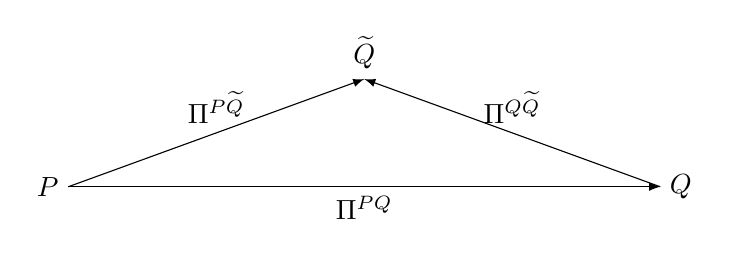
\begin{tikzpicture}
	\path (0,0) coordinate[label=left:$\mathbb{P}$]  (A) --(20:4) coordinate[label=above:$\widetilde{\mathbb{Q}}$] (C) -- ++(-20:4) coordinate[label=right:$\mathbb{Q}$] (B);
	\draw[-latex] (A) -- (B);
	\draw[-latex] (A) -- (C);
	\draw[-latex] (B) -- (C);
	\path (A) -- (B) node[midway,below] {$\Pi^{\mathbb{P}\mathbb{Q}}$};
	\path (A) -- (C) node[midway,above] {$\Pi^{\mathbb{P}\widetilde{\mathbb{Q}}}$};
	\path (C) -- (B) node[midway,above] {$\Pi^{\mathbb{Q}\widetilde{\mathbb{Q}}}$};
	\end{tikzpicture}
	\caption{Considered measure changes between the physical measure $\mathbb{P}$, the artificial risk-neutral measure $\mathbb{Q}$, and the swap's pricing measure $\widetilde{\mathbb{Q}}$ as well as their connections with the true market prices of risk $\Pi^{\mathbb{P}\mathbb{Q}}$, the classical market price of risk $\Pi^{\mathbb{P}\widetilde{\mathbb{Q}}}$, and the MPDP denoted by$\Pi^{\mathbb{Q}\widetilde{\mathbb{Q}}}$.}
	\label{fig:OverviewMeasureChanges}
\end{figure}


Indeed, the MPDP is triggered by typical features of the electricity market entering the swap's volatility.
In particular, delivery-dependent effects like seasonalities and term-structure effects play a crucial role.
\cite{fanelli2019seasonality} empirically identify seasonalities in the swap's delivery period by considering implied volatilities of electricity options.
Renewable energy, like wind and solar energy, intensify especially the seasonal effects mentioned before. 
%Hence, the higher the market share of renewables, the more pronounced the MPDP will be. This applies especially for Germany, having ambitious plans for future investments in renewable energy.
An additional property of electricity and commodity markets is the Samuelson effect (see \cite{Samuelson}): The closer we reach the end of the maturity, the more effect the volatility has.
\cite{BenthParaschiv} and \cite{JaeckLautier} provide empirical evidence for the Samuelson effect in the volatility term-structure of electricity swaps. It can also be  observed in the implied volatilities of electricity options, especially far out and in the money (see \cite{kiesel}).
\cite{Kemper2022} characterize the MPDP for such seasonalities and term-structure effects within a stochastic volatility model through the variance per unit of expectation of the delivery-dependent effects.
We contribute to the literature by investigating the MPDP analytically, affected by seasonalities and the Samuelson effect. Moreover, we lay the foundation for the empirical analysis of the MPDP.\\


Further characteristics of the electricity swap market are mean-reversion and jump behavior.
As mentioned by \cite{Latini2019} and \cite{KleisingerYu} among others, mean-reversion is an important property of the electricity swap prices. 
\cite{KoekebakkerOllmar} empirically validate that the short-term price varies around the long-term price, which confirms mean-reverting behavior.
As \cite{Benth2019}, we face the problem of changing a mean-reverting process to the risk-neutral measure.
We extend their measure change to the geometric setting. We even provide a proof  for stochastic volatility settings in order to address models such as \cite{Kemper2022} and \cite{schneider2018samuelson}.
Besides mean-reversion, \cite{Benth2019} include jumps as an outstanding characteristic of electricity prices. 	In particular, they consider compound Poisson processes under the physical measure in a mean-reverting, arithmetic setting.
While adjusting the paper by \cite{Kemper2022} to jumps, we establish the \textit{MPDP of jump risk} whenever the jump coefficient relies on delivery-dependent effects. \\
%\cite{KleisingerYu} stress that jumps are only affecting short-term futures but not on the long run. 
%Moreover, \cite{Kemper2022} observe a smile effect in options on electricity swaps motivating their stochastic volatility model but also justifying jump fears.\\

%In our empirical analysis, we investigate twelve  swap contracts with monthly delivery from January to December 2019. Each swap is treated as a separate contract assuming that it is driven by an independent Brownian motion. 
%%We present two types of delivery-dependent functions entering in two models separately. 
%To this data, we fit a model indicating seasonality effects in the volatility coefficient. On the other hand, we estimate the parameters of a Samuelson type model. In order to avoid overfitting, we restrict ourselves to separate effects and do not consider joint effects. The estimation procedure is split in two steps: In a first step, we identify jumps for each contract using a thresholding technique. In a second step, we give the model's jump free likelihood to fit the remaining parameters by Maximum-Likelihood-Estimation (MLE). Note that we do not perform a term-structure fit by estimating all swap prices occurring at a fixed day since the presence of parallel contracts is limited.
%The objective of our analysis is not to perform an
%exhaustive empirical study of swap price modeling but to provide evidence for the MPDP. \\

%\discuss{Discussion of MPDP spread Theory /praxis?}
%Last but not least, the delivery period itself needs to be implemented into the swap as a fundamental feature since it presents the foundation of the swap price derivation.
%We mainly distinguish between two lines of literature: first, the \textit{classical} spot based approach and second, the \textit{alternative} futures based approach.
%Depending on the methodology, the electricity swap results from averaging the spot or futures price with respect to the delivery time.

%The \textit{classical approach} is based on exogenous dynamics for the spot price modeling the day-ahead electricity price (see, e.g., \Cref{tab:ClassificationSwapPriceModels} for arithmetic and geometric settings, and \cite{KleisingerYu} for a multi-factor polynomial setting).
%Following the classical approach, stylized facts of the spot are automatically included at the level of the swap price. 
%Some references however doubt that the swap price evolves dependently on the spot (see, e.g., \cite{Aid2015}). Therefore, it could be misleading to apply the classical approach in electricity markets.
%The \textit{alternative approach} directly specifies the futures price instead of introducing a day-ahead spot price. 
%This is also known as a market model and goes back to the famous model by \cite{HJM}. 
%As far as we know, the alternative approach was firstly connected to energy-related derivatives by \cite{ClewlowStrickland1999} and to electricity derivatives by \cite{Bjerksund} followed by a row of works (see, e.g., \Cref{tab:ClassificationSwapPriceModels} for arithmetic and geometric settings, and \cite{Hinderks2020} for a structural model and \cite{CuchieroPersioGuidaSvalute2022} for measure-valued processes).
%They propose a Heath-Jarrow-Morton-style model including seasonal pattern using a deterministic decreasing convex volatility function in time and analyze the corresponding option price.
%\cite{KoekebakkerOllmar} investigate swaps in the Nordic electricity market from 1995-2001 proposing a geometric setting for the swap and analyze the swap's volatility factor structure. They validate that the short-term price varies around the long-term price which also confirms mean-reverting behavior.
%\cite{BenthKoekebakker2008} discuss the volatility and price structure for the electricity swap based on the geometric futures price dynamics and provide a non-Markovian dynamics, which is proposed to be approximated as in \cite{Bjerksund}.
%\cite{Latini2019} propose an additive no-arbitrage model for the futures and confirm mean-reverting features, seasonalities and volatility-term structure while investigating electricity swaps at the German EEX.
%\cite{Benth2019} go further and introduce jumps to the additive HJM-style setting.

%\textit{Arithmetic averaging} is the classical way to implement the swap's delivery period and is tailor-made for arithmetic price dynamics. In particular, continuous arithmetic averaging is applied by \cite{Bjerksund}, \cite{KoekebakkerOllmar}, \cite{Benth2007}, \cite{Benth2008}, \cite{Benth2014}, \cite{Latini2019}, \cite{Benth2019}, \cite{KleisingerYu}, among others. For discrete arithmetic averaging, we refer to \cite{LuciaSchwartz2002} and \cite{BurgerMuller2004}.
%Instead, arithmetic averaging of geometric price dynamics  is poorly suited since the resulting swap price dynamics are neither geometric nor Markovian.
%It requires an approximation of the swap price volatility introduced by \cite{Bjerksund} whenever we want to consider tractable swap price dynamics (see also \cite{Benth2008}, \cite{BenthKoekebakker2008}).
%In the following, we call this procedure the \textit{approximated averaging} since it is the arithmetic average of approximated logarithmic returns.
%In contrast, \textit{geometric averaging} is the arithmetic average of logarithmic returns and directly leads to suitable geometric dynamics without any need for approximations whenever the price dynamics are of geometric type (see \cite{Kemper2022}).
%Since we do not observe any negative prices in our dataset, we stick to a geometric setting and compare the ladder averaging procedures.\\


%We thereby allow for typical features of the electricity swap market. Beyond the delivery period, our model is feasible to cover term-structure effects, seasonalities, mean-reversion, and jump behavior. In particular, seasonalities play a crucial role in the electricity market. \cite{fanelli2019seasonality} identify especially seasonalities in the delivery period of swaps.
%As mentioned by \cite{GemanRoncoroni} and \cite{FilipovicLarssonWare2018} among others, mean-reversion is another important property of the electricity spot prices. \cite{Latini2019}?
%This feature is also translated into electricity futures and swap prices as adopted in \cite{KoekebakkerOllmar}, \cite{KleisingerYu}.  Besides mean-reversion, \cite{Benth2019} include jumps as an outstanding characteristic of electricity prices. 	In particular, they consider compound Poisson processes under the physical measure in a mean-reverting arithmetic setting.
%\cite{KleisingerYu} stress that jumps are only affecting short-term futures but not on the long run. 
%Moreover, \cite{Kemper2022} observe a smile effect in options on electricity swaps motivating their stochastic volatility model. However, there might be several further reasons for the smile effect such as transaction costs, ambiguity, or jump fears.
%Finally, a well-known feature in electricity- and commodity markets is the Samuelson effect (see \cite{Samuelson}), which is identified in electricity futures for example by \cite{BenthParaschiv} and \cite{JaeckLautier}. The effect implies that futures close to delivery are much more volatile than are those whose expiration date lies far off.
%This effect can be observed in the implied volatility of electricity options, especially  far out and in the money  (see also \cite{Kemper2022} and  \cite{kiesel} ).
%The effect is typically included in any electricity futures price dynamics.  \cite{schneider2018samuelson} include such a term-structure effect within the framework of stochastic volatility modeling applied to agricultural futures. \cite{schmeck2016} investigates analytically the impact of the Samuelson effect on option pricing.
% due to a  drift term in the dynamics that is characterized by the variance of the weighted delivery standardized by its expectation and the difference between the averaged cumulant of the futures and the cumulant of the swap. This drift is used to define  the additional market price of risk for delivery periods and an equivalent martingale measure ${\mathbb{Q}}$ for the swap price.  ${\mathbb{Q}}$ can thus be used as a pricing measure for derivatives on the swap. 


%In this paper, we investigate modeling the delivery period explicitly through a continuous weighted averaging approach for futures prices of the geometric type, in line with \cite{Kemper2022} and \cite{Bjerksund}. 
%Both approaches lead directly to Markovian and geometric swap price dynamics.
%We discuss similarities and differences between both approaches and introduce a numéraire caused by a different averaging techniques. 
%Indeed, the geometric averaging of futures prices coincides with the arithmetic averaging procedure applied to logarithmic futures prices.
%Hence, the geometric average is tailor-made for relative growth rate models.
%In line with the market model approach, we base the averaging procedure on an artificial futures contract that is a martingale under the artificial  risk-neutral measure $\mathbb{Q}$. The swap based on the approximated version is a martingale as well. In contrast, the resulting swap price dynamics based on geometric averaging are not a martingale under $\mathbb{Q}$ leading to the MPDP of diffusion and jump risk and a new pricing measure $\widetilde{\mathbb{Q}}$ which can thus be used to price derivatives on the swap.
%A decomposition of the market price for electricity swaps arises when turning to the physical measure $\mathbb{P}$  to investigate our proposed model empirically. \Cref{fig:OverviewMeasureChanges} gives an overview over the connections between the different measures $\mathbb{P}$, $\mathbb{Q}$, and $\widetilde{\mathbb{Q}}$ and their corresponding market prices of risk $\Pi^{\mathbb{P}\mathbb{Q}}$ and $\Pi^{\mathbb{P}\widetilde{\mathbb{Q}}}$ and the MPDP $\Pi^{\mathbb{Q}\widetilde{\mathbb{Q}}}$.

%Moreover, we compare the swap price resulting from the approximated averaging which causes higher electricity swap prices. As a consequence, we can show that the precise swap price is lower than the one resulting from approximated averaging.
%Note that we exclude for simplicity the presence of overlapping contracts like quarterly or yearly electricity swap contracts. To tackle this issue, we refer to \cite{Kemper2022}.



The contribution to the literature is twofold: 
First, we adjust the paper by \cite{Kemper2022} to the jump case under the artificial risk-neutral measure leading to an extended characterization of the MPDP regarding diffusion \textit{and} jump risk. Hence, even if approximated averaging in the spirit of \cite{Bjerksund} is performed in a Merton type model, the model can easily overcome any approximation issues through an application of the MPDP.
Second, we transfer the model to the physical measure and compare the swap prices resulting from geometric  and approximated  averaging
as well as their risk-neutral measures revealing the decomposition of the market price of risk into the classical one and the MPDP. Consequently, the model lays the foundation for empirical investigations in the future. \\
%Third, we investigate the model empirically and provide empirical evidence for the MPDP in the case of two separate delivery-dependent volatility effects.\\

The paper is organized as follows: 
\Cref{sec:AVERAGING} presents the geometric averaging approach under the artificial risk-neutral measure applied to the jump-type futures curve. In addition, it presents the  MPDP of diffusion and jump risk. 
\Cref{sec:Model} introduces the model under the physical measure and identifies the decomposition of the market price of risk.
%The  estimation procedure and the empirical findings are presented in \Cref{sec:EmpiricalInvestigation}.
Finally, \Cref{sec:summary} concludes our main findings. 



\section{On the MPDP of Diffusion and Jump Risk} \label{sec:AVERAGING} 
We particularly focus on an electricity swap contract delivering  1 MWh of electricity during the agreed delivery period $(\tau_1,\tau_2]$. 
At a trading day $t\leq \tau_1$ before the contract expires,  we denote the swap price by $F(t, \tau_1,\tau_2)$ settled such that the contract is entered at no cost. 
It can be interpreted as an average price of instantaneous delivery. Motivated by this interpretation, we consider an artificial futures contract with price $f(t,\tau)$ that stands for instantaneous delivery at time $\tau\in(\tau_1,\tau_2]$. Note that such a contract does not exist on the market  but it turns out to be useful for modeling purposes when considering delivery periods (see, e.g., \cite{Benth2019} and \cite{Kemper2022}). \\

Following the approach by \cite{HJM}, we derive the price of an electricity swap contract based on an instantaneous futures price model.
More precisely, we compare two types of swap prices resulting from geometric and approximated averaging. The goal of this section is to investigate the pricing spread between both approaches in order to quantify the consequences of the approximation and thus the effect of the precise geometric averaging procedure. As the pricing spread goes along with different risk-neutral measures, we additionally investigate the distance of both risk-neutral measures quantified by the MPDP. Moreover, we characterize the MPDP for specific volatility functions and different jump size distributions.

% \discuss{Begründung warum wir das machen. Relevance of investigation.} 

\paragraph{The Model.}
Consider a filtered probability space $(\Omega, \mathcal{F}, (\mathcal{F}_t)_{t\in[0,\tau]},\mathbb{Q})$,
where the filtration satisfies the usual conditions.
We first model the solution of a futures contract and then derive the corresponding dynamics to avoid lacks of existence in the presence of jumps (see \cite{Papapantoleon}). At time $t\leq\tau$, let the logarithmic price process of the futures contract be defined as
	\begin{align}
	\ln f(t,\tau) &= \ln f(0,\tau)+ \int_{0}^{t}\sigma(s,\tau)dW^{\mathbb{Q}}_s
	+\int_{0}^{t}\eta(s,\tau)  d\widetilde{J}^{\mathbb{Q}}_s - \int_{0}^{t}c^{\mathbb{Q}}(s,\tau)ds\;, \label{eq:futuresQsol1}
	\end{align}
 % \begin{align}
	% \ln f(t,\tau) &= \ln f(0,\tau)+ Y(t,\tau)\;, \label{eq:futuresQsol1}\\
	% Y(t,\tau)&=\int_{0}^{t}\sigma(s,\tau)dW^{\mathbb{Q}}_s
	% +\int_{0}^{t}\eta(s,\tau)  d\widetilde{J}^{\mathbb{Q}}_s - \int_{0}^{t}c^{\mathbb{Q}}(s,\tau)ds\;, \label{eq:YunderQ}
	% \end{align}
 with initial non-random conditions $f(0,\tau) >0$.	
	Moreover, $W^{\mathbb{Q}}$ is a one-dimensional standard Brownian motion under $\mathbb{Q}$ independent of the jump process $\widetilde{J}^{\mathbb{Q}}$. 
	In particular, $\widetilde{J}^{\mathbb{Q}}$ is a compound compensated jump process defined through the compensated Poisson random measure $\widetilde{N}^{\mathbb{Q}}(dt,dz)=N(dt,dz)-\ell^{\mathbb{Q}}(dz)dt$:
	\begin{align}
	\widetilde{J}^{\mathbb{Q}}_t=\int_{0}^{t}\int_{\mathbb{R}}z\widetilde{N}^{\mathbb{Q}}(ds,dz)\;,
	\end{align}
	with Lévy measure $\ell^{\mathbb{Q}}(dz)=\lambda^{\mathbb{Q}} G(dz)$, which is independent of the delivery time, and where $\lambda^{\mathbb{Q}}>0$ indicates the jump intensity and $G(dz)$ the jump size distribution.
	The last term in \Eqref{eq:futuresQsol1} defines the compensator of the logarithmic return under the current measure $\mathbb{Q}$:
	\begin{align}
	c^{\mathbb{Q}}(t,\tau)=\frac12\sigma^2(t,\tau)+ \psi^{\mathbb{Q}}(i\eta(t,\tau))\;, \label{eq:compensator}
	\end{align}
	where $\psi^{\mathbb{Q}}(ir)$ is the integrand of the Lévy-Khintchine exponential defined through the moment generating function 
	\begin{align}
	\psi^{\mathbb{Q}}(r):=\int_{\mathbb{R}}\left(e^{rz}-1-rz\right)\ell^{\mathbb{Q}}(dz)\;.
	\end{align}
	We assume that the futures price volatility and jump coefficients, $\sigma(t,\tau)$ and $\eta(t,\tau)$, are deterministic and that the futures price $f(t,\tau)$  is $\mathcal{F}_t$-adapted for $t\in[0,\tau]$. We further assume that they satisfy suitable integrability and measurability conditions (see  \Cref{ass:TechnicalRequirementsQ1} in Appendix \ref{app:tech_requ3} for details) to ensure that the process in \Eqref{eq:futuresQsol1} is a $\mathbb{Q}$-martingale, and that \Eqref{eq:futuresQsol1} gives the unique solution to the process evolving as
	\begin{align}
	\frac{df(t,\tau)}{f(t-,\tau)}= \sigma(t,\tau)dW^{\mathbb{Q}}_t+\int_{\mathbb{R}}\left(e^{\eta(t,\tau)z}-1\right)\widetilde{N}^{\mathbb{Q}}(dt, dz)\;. \label{eq:futuresQ}
	\end{align}
As $\sigma(t,\tau)$ depends on both, trading time $t$ and delivery time $\tau$, we allow for volatility structures as the Samuelson effect or seasonalities in the delivery time, which are addressed in \Cref{Ex:Seasonality,Ex:Samuelson}.

\paragraph{Implementing the Delivery Period.}
Following the Heath-Jarrow-Morton approach to price futures and swaps in electricity markets, the swap price is usually defined as the \textit{arithmetic weighted average} of futures prices (see, e.g., \cite{Benth2008},  \cite{Bjerksund}, and \cite{Benth2019}):
\begin{equation} \label{eq:arithmeticnoarbitrage}
F^A(t,\tau_1,\tau_2):=\int_{\tau_1}^{\tau_2}w(u, \tau_1, \tau_{2})f(t,u)du\;, 
\end{equation} 
for a general weight function
\begin{align}
w(u,\tau_1, \tau_2):=\frac{\hat{w}(u)}{\int_{\tau_1}^{\tau_2}\hat{w}(v)dv}\;, ~~~~ \text{for } u\in(\tau_1,\tau_2]\;, \label{eq:weights}
\end{align}
where $\hat{w}(u)>0$ is the corresponding settlement function.
Note that $w$ defines a probability density function with support on $(\tau_1,\tau_2]$ since it is positive and integrates to one, that is $\int_{\tau_1}^{\tau_2}w(u,\tau_1, \tau_2)du=1$.
Hence, we denote $U$ as a random delivery variable with density $w(u,\tau_1,\tau_2)$ (see also \cite{Kemper2022}).
The most popular example is given by a constant settlement type $\hat{w}(u) =1$, such that the density becomes $w(u,\tau_1, \tau_2)= \frac{1}{\tau_2 - \tau_1}$ and $U\sim \mathcal{U}((\tau_1,\tau_2])$ is uniformly distributed over the delivery period. This corresponds to a one-time settlement. A~continuous settlement over the time interval $(\tau_1,\tau_2]$ is covered by a continuous discount function $	\hat{w}(u) =e^{-ru}$, where $r$ is the constant interest rate (see, e.g., \cite{Benth2008}). \\

The arithmetic average of the futures price as in \Eqref{eq:arithmeticnoarbitrage} leads to tractable dynamics for the swap as long as one  assumes an arithmetic structure of the futures prices as well. 
This is based on the fact that arithmetic averaging is tailor-made for absolute growth rate models.
Nevertheless,  if one defines the futures price as a geometric process as in \Eqref{eq:futuresQ}, one can show that the dynamics of the swap price $F^A$ defined through \Eqref{eq:arithmeticnoarbitrage} are given by
\begin{equation}
\begin{split}
\frac{dF^A(t,\tau_1,\tau_2)}{F^A(t-,\tau_1,\tau_2)}=&~\Big[\sigma(t,\tau_2) -\int_{\tau_1}^{\tau_2}\frac{\partial \sigma}{\partial u}(t,u)\frac{w(\tau, \tau_1,\tau_2)}{w(\tau, \tau_1, u)} \frac{F^A(t, \tau_1,u)}{F^A(t, \tau_1,\tau_2)} du\Big] ~dW^\mathbb{Q}_t\\
&~+ \int_{\mathbb{R}}\Big(e^{\eta(t,\tau_2)z}-1- \int_{\tau_1}^{\tau_2}\frac{\partial e^{\eta(s,u)z}}{\partial u}\frac{w(\tau, \tau_1,\tau_2)}{w(\tau, \tau_1, u)}\frac{F^A(t, \tau_1,u)}{F^A(t, \tau_1,\tau_2)} du\Big)~\widetilde{N}^{\mathbb{Q}}(dz,dt)\;,
\end{split}
\end{equation}
for any $\tau\in(\tau_1,\tau_2]$ (see \cite{Benth2008}, cf.\ Chapter 6.3.1). Thus, the dynamics of the swap price is neither a geometric process nor Markovian, which makes it unhandy for further analysis.  
To overcome this issue, \cite{Bjerksund} suggest an approximation in the setup without jumps, which we call \textit{approximated averaging} since it is the arithmetic average of approximated logarithmic returns. Approximated averaging maintains the martingale property
meaning that the swap is a martingale whenever $f$ is a martingale. 
If we transfer the approximated averaging procedure to our jump setting, we can define the  swap price process based on approximated averaging by
\begin{align}
\frac{dF^a(t,\tau_1,\tau_2)}{F^a(t-,\tau_1,\tau_2)}:=\int_{\tau_1}^{\tau_2}w(u,\tau_1,\tau_2) \frac{df(t,u)}{f(t-,u)} du\;. \label{eq:arithAverage_drift}
\end{align}
In contrast, \textit{geometric averaging} originates from the arithmetic average of logarithmic returns without any need for approximations.
Hence, in line with \cite{Kemper2022}, we define the swap price originating from geometric averaging by
\begin{align}
F(t,\tau_1,\tau_2):=e^{\int_{\tau_1}^{\tau_2}w(u,\tau_1,\tau_2)\ln f(t,u)du}\;, \label{eq:GeomAverage}
\end{align}
(see also \cite{KemnaVorst1990}).
Assume that the volatility and jump coefficients satisfy further integrability conditions (see \Cref{ass:TechnicalRequirementsQ2} in \Cref{app:tech_requ3}).
It turns out, that the resulting swap price dynamics is a geometric process with a non-zero drift term:
\begin{Lemma}[The Swap Price under $\mathbb{Q}$] \label{lemma:dyn_Swap_Q}
	Let  \Cref{ass:TechnicalRequirementsQ2} in \Cref{app:tech_requ3} be satisfied.
	Under the artificial pricing measure $\mathbb{Q}$, the dynamics of the swap price process $F(\cdot,\tau_1, \tau_2)$, defined in \Eqref{eq:GeomAverage}, are given by
	\begin{equation}\label{eq:FunderQ}
	\begin{split}
	\frac{d F(t,\tau_1,\tau_2)}{F(t-,\tau_1,\tau_2)} =&~
	\mathbb{E}[\sigma(t,U)]~dW^{\mathbb{Q}}_t+\int_{\mathbb{R}} \left(e^{\mathbb{E} [\eta(t,U)]z}-1\right)\widetilde{N}^{\mathbb{Q}}(dt,dz)\\
	&~-\left(\frac{1}{2}\mathbb{V} \left[\sigma(t,U) \right]
	+\mathbb{E} [\psi^{\mathbb{Q}}(\eta(t,U))]-\psi^{\mathbb{Q}}(\mathbb{E} [\eta(t,U)]) \right) dt\;,
	\end{split}
	\end{equation}
	where $U$ denotes the random delivery variable  with density $w(u,\tau_1,\tau_2)$.
\end{Lemma}
\begin{proof}
	Plugging the integral representation of the futures rate process from \Eqref{eq:futuresQsol1} into \Eqref{eq:GeomAverage} 
  gives us $F(t,\tau_1,\tau_2)
	=F(0, \tau_1, \tau_{2}) e^{\bar{X}(t,\tau_1,\tau_2)}$,
	% \begin{align*}
	% F(t,\tau_1,\tau_2)
	% =F(0, \tau_1, \tau_{2})
	% e^{\int_{\tau_1}^{\tau_2}w(u, \tau_1, \tau_{2})Y(t,u)du}\;. 
	% \end{align*}
	% where $\bar{X}(t,\tau_1, \tau_{2}) := \int_{\tau_1}^{\tau_2}w(u, \tau_1, \tau_{2})\ln f(t,u)du$ is the swap price rate.
	% using the integral representation of the futures rate process from \Eqref{eq:futuresQsol1}
 where an application of the stochastic Fubini Theorem (see \cite{Protter2005}, cf.\ Theorem~65, Chapter IV.6) leads to
	\begin{align}
	\bar{X}(t,\tau_1,\tau_2)=&\int_{0}^{t}\mathbb{E} \Big[\sigma(s,U)\Big]dW^{\mathbb{Q}}_s+\int_{0}^{t}\mathbb{E} [\eta(s,U)]d\widetilde{J}^{\mathbb{Q}}_s-\frac12\int_{0}^{t}\mathbb{E} \Big[\sigma^2(s,U)\Big]ds
	-\int_{0}^{t}
	\mathbb{E} [\psi^{\mathbb{Q}}( \eta(s,U))]ds\;. \label{eq:Xbar}
	\end{align}
	Then, \Eqref{eq:FunderQ} follows using Itô's formula (see, e.g., \cite{OksendalSulem}). \qed\\
\end{proof}

Having presented the three procedures of continuous time averaging that are used to derive the swap from an underlying artificial futures curve, we would like to compare them:
Arithmetic averaging, defined by \Eqref{eq:arithmeticnoarbitrage}, is tractable for arithmetic futures curves, whereas approximated averaging, defined by \Eqref{eq:arithAverage_drift}, and geometric averaging, defined by \Eqref{eq:GeomAverage}, are well suited for geometric futures curves.
In line with a series of literature (see \Cref{tab:ClassificationSwapPriceModels}), we follow the geometric approach.
Our goal throughout this paper is to investigate the pricing spread between geometric and approximated averaging analytically.

\paragraph{The MPDP.}
Although the futures price $f$ and the approximated $F^a$ are martingales under the pricing measure $\mathbb{Q}$, the swap price $F$ is not a $\mathbb{Q}$-martingale: Indeed, the swap price process under $\mathbb{Q}$ has a negative drift term consisting of two parts given by the swap's variance and the difference between the averaged Lévy-Khintchine integrand and the Lévy-Khintchine integrand of the averaged jump coefficient.
Hence, using geometric averaging leads to a new interpretation of risk related to the delivery period as we will analyze in the following.\\

%\section{Additional Measure Change}\label{sec:AdditionalMgMeasure}
Analogous to \cite{Kemper2022}, we derive the corresponding risk-neutral measure $\widetilde{\mathbb{Q}}$ under which the electricity swap price $F$ is a martingale.
For deriving the swap's risk-neutral measure, we thus define the MPDP extended to jumps in the following.
\begin{Definition}[The MPDP] \label{Def_MPDP}
At time $t\in[0,\tau_1]$, the \textit{market price of diffusion and jump risk for delivery periods} associated to the delivery period $(\tau_1,\tau_2]$ is defined by
$\Pi^{\mathbb{Q}\widetilde{\mathbb{Q}}}:=(\Pi_1^{\mathbb{Q}\widetilde{\mathbb{Q}}},\Pi_2^{\mathbb{Q}\widetilde{\mathbb{Q}}})$, where
\begin{align}
&\Pi_1^{\mathbb{Q}\widetilde{\mathbb{Q}}}(t,\tau_1,\tau_2) :=-\frac12 \frac{\mathbb{V} \left[\sigma(t,U)\right]}{\mathbb{E} \left[\sigma(t,U)\right]}\;, \label{eq:AddMP1}\\
&\Pi_2^{\mathbb{Q}\widetilde{\mathbb{Q}}}(t, \tau_1,\tau_2):= 
%-\frac{\mathbb{E} [\psi^{{\mathbb{Q}}}(\eta(t,U))]- \psi^{{\mathbb{Q}}}(\mathbb{E}[\eta(t,U)])}{\int_{\mathbb{R}}\left(e^{\mathbb{E} [\eta(t,U)]z}-1\right)\ell^{\mathbb{Q}}(dz) } 
% = 
- \frac{\int_{\mathbb{R}}\mathbb{E} [e^{\eta(t,U)z}]-e^{\mathbb{E} [\eta(t,U)]z}\ell^{\mathbb{Q}}(dz)}{\int_{\mathbb{R}}\left(e^{\mathbb{E} [\eta(t,U)]z}-1\right)\ell^{\mathbb{Q}}(dz)}\;.\label{eq:AddMP2}
\end{align}
\end{Definition}
In general, the MPDP does not coincide with the market price of risk. In fact, it is an additional risk that has to be taken into account whenever approximated averaging is conducted.
Technically speaking, the MPDP characterizes the distance between the martingale measure of the swaps, $F$ and $F^a$, resulting from geometric and approximated averaging.
In particular, $\Pi_1$ refers to the additional diffusion risk, which is measurable and $\mathcal{F}_t$-adapted as $\sigma(t,u)$ is. 
It can be interpreted as the trade-off between the weighted average variance of a stream of futures, on the one hand, and the variance of the swap, on the other hand (see also
\cite{Kemper2022} for an elaboration of the MPDP $\Pi_1^{\mathbb{Q}\widetilde{\mathbb{Q}}}$ and a detailed interpretation).
$\Pi_2^{\mathbb{Q}\widetilde{\mathbb{Q}}}$ is the additional jump risk, which is the difference between the Lévy-Khintchine integrands standardized by the swap's jump coefficient.
\begin{Remark} \label{re:1}
	\begin{itemize}
	\item[$(i)$] Note that $\Pi^{\mathbb{Q}\widetilde{\mathbb{Q}}}$ would be zero, whenever the volatility and jump coefficients are independent of delivery time. For this reason, we call  $\Pi^{\mathbb{Q}\widetilde{\mathbb{Q}}}$ the \textit{market price of  risk for delivery periods} (MPDP).
	\item[$(ii)$] The MPDP of diffusion and jump risk is strengthened by delivery-dependent effects within the volatility and jump coefficients. For example, pronounced term-structure effects or seasonalities in the delivery period within these coefficients capture a distinct dependence on the delivery period and, consequently, lead to a high MPDP (see also \Cref{Ex:Seasonality,Ex:Samuelson} for the MPDP of diffusion risk and \Cref{ex:JumpsNormal,ex:JumpsExponential}.
	\item[$(iii)$] $\Pi_1^{\mathbb{Q}\widetilde{\mathbb{Q}}}$ is in line with the MPDP for diffusion risk found in \cite{Kemper2022}, where a stochastic volatility scenario is considered.
	\end{itemize}
\end{Remark} 

In a next step, we would like to characterize the MPDP of diffusion risk $\Pi^{\mathbb{Q}\widetilde{\mathbb{Q}}}_1$ more explicitly.
The MPDP of diffusion risk arises through delivery-dependent volatility effects such as seasonality in delivery periods and the Samuelson effect (see \cite{Kemper2022}). We state the corresponding MPDP in the following two examples while assuming a one-time settlement such that $w(t,\tau_1,\tau_2)=\frac{1}{\tau_2-\tau_1}$.% and $\sigma(t,u)\equiv 1$.

\begin{Example}[Seasonal Volatility]\label{Ex:Seasonality}
Inspired by \cite{fanelli2019seasonality}, we capture seasonality in the delivery period by incorporating a trigonometric function into the futures volatility  $\sigma(t,u)=S_1(u)$ in (see \Eqref{eq:AddMP1}) given by
\begin{align}
S_1(u):= a+ b \cos (2\pi (u+c))\;,
\end{align}
for $a>b>0$ and $c\in[0,1)$.
According to \Cref{Def_MPDP}, this leads to a MPDP of diffusion risk of the following form
\begin{align}
\Pi_1^{\mathbb{Q}\widetilde{\mathbb{Q}}}(t,\tau_1,\tau_2)=-\frac12\frac{\mathbb{V}[S_1(U)]}{\mathbb{E}[S_1(U)]}\;,
\end{align}
where 
\begin{align}
\mathbb{E}[S_1(U)]&= a+\frac{b}{2\pi (\tau_2-\tau_1)} \Big[\sin(2\pi(u+c))\Big]^{u=\tau_2}_{u=\tau_1}\;, \label{eq:Es}\\
\mathbb{E}[S_1(U)^2]&= a^2+\frac{b^2}{2}+\frac{ab}{\pi(\tau_2-\tau_1)}\Big[\sin(2\pi(u+c))\Big]^{u=\tau_2}_{u=\tau_1}+\frac{b^2}{8\pi(\tau_2-\tau_1)}\Big[\sin(4\pi(u+c))\Big]^{u=\tau_2}_{u=\tau_1}\;. \label{eq:Es2}
\end{align}
\end{Example}

\begin{Example}[Term-Structure Volatility]\label{Ex:Samuelson}
We implement the Samuelson effect as in \cite{schneider2018samuelson} into the futures volatility $\sigma(t,u)=S_2(u-t)$ (see \Eqref{eq:AddMP1}) through an exponential function with exponential damping factor $\Lambda>0$ and terminal volatility $\bar{\lambda}>0$ given by
\begin{align}
	S_2(u-t):=\bar{\lambda}e^{-\Lambda(u-t)}\;.
\end{align}
According to \Cref{Def_MPDP}, this leads to a MPDP of diffusion risk of the following form
\begin{align}
\Pi_1^{\mathbb{Q}\widetilde{\mathbb{Q}}}(t,\tau_1,\tau_2)=-\frac12\frac{\bar{\bar{\Lambda}}-\bar{\Lambda}^2}{\bar{\Lambda}}e^{-\Lambda(\tau_1-t)}\;,
\end{align}
for constant parameters $\bar{\Lambda}:=\frac{\bar{\lambda}(1-e^{-\Lambda(\tau_2-\tau_1)})}{\Lambda (\tau_2-\tau_1)}$ and $ \bar{\bar{\Lambda}}:=\frac{\bar{\lambda}^2(1-e^{-2\Lambda(\tau_2-\tau_1)})}{2\Lambda (\tau_2-\tau_1)}$ implicitly depending on the delivery period.
\end{Example}
Hence, the MPDP of diffusion risk is constant for a fixed contract in \Cref{Ex:Seasonality}, whereas the Samuelson effect remains still visible in \Cref{Ex:Samuelson}. For a detailed investigation of the volatility term structure, we refer to \cite{Kemper2022}. \\

The MPDP of jump risk is triggered by delivery-dependent jump effects.
For notational convenience, we choose $\eta(t,u)$ independent of trading time and again assume a one-time settlement.
In the following examples, we characterize the MPDP of jump risk and the spread based on two suitable jump size distributions: Normal and exponential.
We also state corresponding moments of the distributions following \cite{GrayPitts2012} (cf.\ Chapter~2).


\begin{Example}[Normal Jump Sizes] \label{ex:JumpsNormal}
 If the jump sizes are normally distributed with $Z\sim\mathcal{N}(\mu_J,\sigma_J^2)$, then the moment generating function is given by
 \begin{align}
 M_Z(\eta)=e^{\mu_J\eta+\frac12 \sigma_J^2\eta^2}\;,
 \end{align}
 such that the MPDP and the spread in Equations~\eqref{eq:AddMP2} and \eqref{eq:Spread2} are given by
	\begin{align}
	{\Pi}^{\mathbb{Q}\widetilde{\mathbb{Q}}}_2(\tau_1,\tau_2)  &= - \frac{\mathbb{E}[e^{\frac12 \eta^2(U)\sigma_J^2+\eta(U)\mu_J}]-e^{\frac12 \mathbb{E}[\eta(U)]^2\sigma_J^2+\mathbb{E}[\eta(U)]\mu_J}}{e^{\frac12 \mathbb{E}[\eta(U)]^2\sigma_J^2+\mathbb{E}[\eta(U)]\mu_J}-1}\;.
	% \bar{\Pi}^{\mathbb{Q}\widetilde{\mathbb{Q}}}_2(\tau_1,\tau_2)  &= - \mu_J\mathbb{E}[\eta(U)]  \frac{\mathbb{E}[e^{\frac12 \eta^2(U)\sigma_J^2+\eta(U)\mu_J}]-e^{\frac12 \mathbb{E}[\eta(U)]^2\sigma_J^2+\mathbb{E}[\eta(U)]\mu_J}}{\left(\mathbb{E}[e^{\frac12 \eta^2(U)\sigma_J^2+\eta(U)\mu_J}]-1\right)\left(e^{\frac12 \mathbb{E}[\eta(U)]^2\sigma_J^2+\mathbb{E}[\eta(U)]\mu_J}-1\right)}\;.
	\end{align}
	The fourth moment is attained by  $\int_{\mathbb{R}}z^4G(dz)=\mu_J^4+ 6\mu_J^2 \sigma_J^2+3\sigma_J^4$.
\end{Example}

%\begin{Example}
%	If the jump sizes are gamma distributed with $Z\sim\mathcal{G}am(a_J,b_J)$ where $a_J$ is the shape parameter and $b_J$ is the rate parameter, for $a_J,b_J>0$, then the moment generating function is given by
%	\begin{align}
%	M_Z(\eta)=\left(1-\frac{\eta}{b_J}\right)^{-a_J}\;,
%	\end{align}
%	for $\eta< b_J$, such that the MPDP and the spread in Equations~\eqref{eq:AddMP2} and \eqref{eq:Spread2} are given by
%	\begin{align}
%	{\Pi}^{\mathbb{Q}\widetilde{\mathbb{Q}}}_2  &= -\frac{\mathbb{E}[M_Z(\eta(U))] -M_Z(\mathbb{E}[\eta(U)])}{M_Z(\mathbb{E}[\eta(U)])-1} \;,\\
%\bar{\Pi}^{\mathbb{Q}\widetilde{\mathbb{Q}}}_2  &= - \mathbb{E}[\eta(U)] \frac{a_J}{b_J} \frac{\mathbb{E}[M_Z(\eta(U))] -M_Z(\mathbb{E}[\eta(U)])}{\left(\mathbb{E}[M_Z(\eta(U))]-1\right)\left(M_Z(\mathbb{E}[\eta(U)])-1\right)}\;,
%	\end{align}
%	defined for $\eta(U)<b_J$ and $\mathbb{E}[\eta(U)]<b_J$.
%	The $n$-th moment is attained by $\int_{\mathbb{R}}z^nG(dz)=\frac{\Gamma(n+a_J)}{b_J\Gamma(a_J)}$, for $n>-a_J$.
%\end{Example}


\begin{Example}[Exponential Jump Sizes] \label{ex:JumpsExponential}
	If the jump sizes are exponentially distributed with
	$Z\sim\mathcal{E}xp(\lambda_J)$, for  $\lambda_J>0$, then the moment generating function is given by
	\begin{align}
	M_Z(\eta)=\left(1-\frac{\eta}{\lambda_J}\right)^{-1}\;,
	\end{align}
	for $\eta<\lambda_J$, such that the MPDP and the spread in Equations~\eqref{eq:AddMP2} and \eqref{eq:Spread2}  are given by
	\begin{align}
	{\Pi}^{\mathbb{Q}\widetilde{\mathbb{Q}}}_2(\tau_1,\tau_2)  &=- \frac{\lambda_J}{\mathbb{E}[\eta(U)]}\left(1-\mathbb{E}\left[\frac{\lambda_J-\mathbb{E}[\eta(U)]}{\lambda_J-\eta(U)}\right]\right) \;,
	% \bar{\Pi}^{\mathbb{Q}\widetilde{\mathbb{Q}}}_2(\tau_1,\tau_2)  &=
	% \frac{\mathbb{E}[\eta(U)]\mathbb{E}[\frac{1}{\lambda_J-\eta(U)}]}{\mathbb{E}[\frac{\eta(U)}{\lambda_J-\eta(U)}]}-1\;,
	\end{align}
	defined for $\eta(U)<\lambda_J$ and $\mathbb{E}[\eta(U)]<\lambda_J$.
	The $n$-th moment is attained by $\int_{\mathbb{R}}z^nG(dz)=\frac{n!}{\lambda_J^n}$ for $n\in\mathbb{N}$. 
 % Note that the parameter in matlab is indicated by the mean $\mu_J=\lambda_J^{-1}$.
\end{Example}

\paragraph{On the Swap's Martingale Measure.}
We define a new pricing measure $\widetilde{\mathbb{Q}}$, such that the swap price process $F(\cdot, \tau_1,\tau_2)$ is a martingale.
Following \cite{OksendalSulem}, define the Radon-Nikodym density through 
\begin{align}
Z^{\mathbb{Q}\widetilde{\mathbb{Q}}}(t,\tau_1,\tau_2) =\prod_{j=1}^{2}
Z_j^{\mathbb{Q}\widetilde{\mathbb{Q}}}(t,\tau_1,\tau_2) \;, \label{eq:densityPtilde}
\end{align}
where
\begin{align}
Z_1^{\mathbb{Q}\widetilde{\mathbb{Q}}}(t,\tau_1,\tau_2)&:=
e^{-\int_{0}^{t}\Pi_1^{\mathbb{Q}\widetilde{\mathbb{Q}}}(s,\tau_1,\tau_2)d\widetilde{W}^{\mathbb{Q}}(s)-\frac{1}{2}\int_{0}^{t}\Pi_1^{\mathbb{Q}\widetilde{\mathbb{Q}}}(s,\tau_1,\tau_2)^2ds}\;,\\
Z_2^{\mathbb{Q}\widetilde{\mathbb{Q}}}(t,\tau_1,\tau_2)&:=
e^{\int_{0}^{t}\int_{\mathbb{R}}\ln(1-\Pi_2^{\mathbb{Q}\widetilde{\mathbb{Q}}}(s, \tau_1,\tau_2))\widetilde{N}^{\mathbb{Q}}(ds,dz)+
	\int_{0}^{t}\int_{\mathbb{R}}\left(\ln(1-\Pi_2^{\mathbb{Q}\widetilde{\mathbb{Q}}}(s, \tau_1,\tau_2))+\Pi_2^{\mathbb{Q}\widetilde{\mathbb{Q}}}(s, \tau_1,\tau_2)\right) \ell^{\mathbb{Q}}(dz)ds}\;.
\end{align}
Assume that 
\begin{align}
\mathbb{E}_{\mathbb{Q}}[Z^{\mathbb{Q}\widetilde{\mathbb{Q}}}(\tau_1,\tau_1,\tau_2)]=1\;, \label{eq:MG_Property}
\end{align}
which means that $Z^{\mathbb{Q}\widetilde{\mathbb{Q}}}(\cdot,\tau_1,\tau_2)$ is indeed a martingale for the entire trading time.
We will show later that the martingale property is satisfied for suitable models such that \Eqref{eq:MG_Property} holds true.
We then define the new measure $\widetilde{\mathbb{Q}}$ through the Radon-Nikodym density
\begin{align}
\frac{d\widetilde{\mathbb{Q}}}{d\mathbb{Q}}=Z^{\mathbb{Q}\widetilde{\mathbb{Q}}}(\tau_1,\tau_1,\tau_2)\;,
\end{align}
which clearly depends on the delivery period $(\tau_1,\tau_2]$. Girsanov's theorem states that if we define the process $W^{\widetilde{\mathbb{Q}}}$ and the random measure $\widetilde{N}^{\widetilde{\mathbb{Q}}}(dt,dz)$ by
\begin{align}
dW^{\widetilde{\mathbb{Q}}}_t&= dW^{\mathbb{Q}}_t +\Pi_1^{\mathbb{Q}\widetilde{\mathbb{Q}}}(t,\tau_1,\tau_2)dt\;, \\
\widetilde{N}^{\widetilde{\mathbb{Q}}}(dt,dz)&= \widetilde{N}^{\mathbb{Q}}(dt,dz)+\Pi_2^{\mathbb{Q}\widetilde{\mathbb{Q}}}(t, \tau_1,\tau_2)\ell^{\mathbb{Q}}(dz)dt\;,
\end{align}
then $W^{\widetilde{\mathbb{Q}}}$ is a Brownian motion under $\widetilde{\mathbb{Q}}$ and $\widetilde{N}^{\widetilde{\mathbb{Q}}}(\cdot,\cdot)$ is the $\widetilde{\mathbb{Q}}$-compensated Poisson random measure of $N(\cdot,\cdot)$  with compensator $\left(1-\Pi_2^{\mathbb{Q}\widetilde{\mathbb{Q}}}(s, \tau_1,\tau_2)\right)\ell^{\mathbb{Q}}(dz)$. 
Under some further  assumptions, ensuring that $Z_2^{\mathbb{Q}\widetilde{\mathbb{Q}}}$ stays positive and that $Z^{\mathbb{Q}\widetilde{\mathbb{Q}}}$ is a true martingale (see \Cref{ass:TechnicalRequirementsQ3} in \Cref{app:tech_requ3}), a straightforward valuation leads  to the following result:
\begin{Proposition}[The Swap Price under $\widetilde{\mathbb{Q}}$] \label{prop:FunderPtilde}
	Let \Cref{ass:TechnicalRequirementsQ3} in \Cref{app:tech_requ3} be satisfied.
	The swap price process $F(\cdot,\tau_1,\tau_2)$, defined in~\eqref{eq:GeomAverage}, is a martingale under $\widetilde{\mathbb{Q}}$. The swap price dynamics are given by
	\begin{align}
	\frac{d F(t,\tau_1,\tau_2)}{F(t-,\tau_1,\tau_2)} = 
	\mathbb{E}[\sigma(t,U)]dW^{\widetilde{\mathbb{Q}}}_t+\int_{\mathbb{R}} \left(e^{\mathbb{E} [\eta(t,U)]z}-1\right)\widetilde{N}^{\widetilde{\mathbb{Q}}}(dt,dz)
	\;,
	\end{align}
	where $W^{\widetilde{\mathbb{Q}}}$ is a Brownian motion under $\widetilde{\mathbb{Q}}$ and $\widetilde{N}^{\widetilde{\mathbb{Q}}}(\cdot,\cdot)$ is the compound compensated Poisson random measure under $\widetilde{Q}$ with Lévy measure $\left(1-\Pi_2^{\mathbb{Q}\widetilde{\mathbb{Q}}}(t, \tau_1,\tau_2)\right)\ell^{\mathbb{Q}}(dz)$ for $t\in[0,\tau_1]$.
\end{Proposition}
\begin{proof}
	We know by definition that $\Pi_1^{\mathbb{Q}\widetilde{\mathbb{Q}}}$ is a continuous adapted process that is square-integrable and $\Pi_2^{\mathbb{Q}\widetilde{\mathbb{Q}}}$ is deterministic and càdlàg in time.
	Hence, all processes are predictable.
	Following \cite{OksendalSulem} (cf.\ Theorem 1.35), we need to show that \Eqref{eq:MG_Property} is satisfied, so that
	$Z^{\mathbb{Q}\widetilde{\mathbb{Q}}}$ is a true martingale.
	Considering the dynamics of $Z^{\mathbb{Q}\widetilde{\mathbb{Q}}}$ using Itô's formula, we have
	\begin{align*}
	d	Z^{\mathbb{Q}\widetilde{\mathbb{Q}}}(t,\tau_1,\tau_2)= 	Z^{\mathbb{Q}\widetilde{\mathbb{Q}}}(t-,\tau_1,\tau_2) \left[-\Pi_1^{\mathbb{Q}\widetilde{\mathbb{Q}}}(t, \tau_1,\tau_2)dW^{\mathbb{Q}}_t-\int_{\mathbb{R}}\Pi_2^{\mathbb{Q}\widetilde{\mathbb{Q}}}(t, \tau_1,\tau_2)z\widetilde{N}^{\mathbb{Q}}(dt, dz)\right]\;,
	\end{align*}
	so that $Z^{\mathbb{Q}\widetilde{\mathbb{Q}}}$ is a local $\mathbb{Q}$-martingale, where $W^{\mathbb{Q}}$ and $\widetilde{N}^{\mathbb{Q}}(\cdot,\cdot)$ are independent of each other.
	Hence, it is enough to show, that $Z_1^{\mathbb{Q}\widetilde{\mathbb{Q}}}$  and $Z_2^{\mathbb{Q}\widetilde{\mathbb{Q}}}$ are true martingales.
	We can prove Novikov's condition regarding the continuous part (see, e.g., \cite{Protter2005}, cf.\ Theorem 41, Chapter III.8) as  $\Pi_1^{\mathbb{Q}\widetilde{\mathbb{Q}}}$:
	\begin{align*}
	\mathbb{E}_{\mathbb{Q}}\left[e^{\frac{1}{2}\int_{0}^{\tau_1}\Pi_1^{\mathbb{Q}\widetilde{\mathbb{Q}}}(s,\tau_1,\tau_2)dW^{\mathbb{Q}}_s}\right]
	=e^{\frac{1}{2}\int_{0}^{\tau_1}\Pi_1^{\mathbb{Q}\widetilde{\mathbb{Q}}}(s,\tau_1,\tau_2)^2ds}<\infty\;.
	\end{align*}
	Hence, $Z_1^{\mathbb{Q}\widetilde{\mathbb{Q}}}$ is a true martingale.
	Moreover, $Z_2^{\mathbb{Q}\widetilde{\mathbb{Q}}}$ is a true martingale under $\mathbb{Q}$ since
	\begin{align*}
	\mathbb{E}_{\mathbb{Q}}[Z_2^{\mathbb{Q}\widetilde{\mathbb{Q}}}(\tau_1,\tau_1,\tau_2)]=
	\mathbb{E}_{\mathbb{Q}}\left[e^{\lambda^{\mathbb{Q}}\int_{0}^{\tau_1}\ln(1-\Pi_2^{\mathbb{Q}\widetilde{\mathbb{Q}}}(s, \tau_1,\tau_2))\widetilde{N}^{\mathbb{Q}}(ds,dz)}\right]
	e^{\int_{0}^{\tau_1}\int_{\mathbb{R}}\left(\ln(1-\Pi_2^{\mathbb{Q}\widetilde{\mathbb{Q}}}(s, \tau_1,\tau_2))+\Pi_2^{\mathbb{Q}\widetilde{\mathbb{Q}}}(s, \tau_1,\tau_2)\right)ds}=1\;,
	\end{align*}
	where the last equality follows from the Lévy-Khintchine representation and  \Cref{ass:TechnicalRequirementsQ3} in \Cref{app:tech_requ3}.
	Hence, we can apply Girsanov's Theorem (see, e.g., \cite{OksendalSulem}, cf.\ Theorem 1.35) and the assertion follows. \qed\\
\end{proof}
Note that the MPDP of diffusion and jump risk, $\Pi_1^{\mathbb{Q}\widetilde{\mathbb{Q}}}$ and $\Pi_2^{\mathbb{Q}\widetilde{\mathbb{Q}}}$, are negative following from Jensen's inequality.
Hence, the geometric averaging technique induces less risk than the application of the approximated arithmetic average for which we need to pay a cost of approximation risk.
%Vice versa, using the geometric average induces less risk than the approximated arithmetic one such that the overall risk is lowered. 

\paragraph{On the Pricing Spread.}
We would like to compare the approximated swap price $F^a$ under $\mathbb{Q}$ with the swap price $F$ under $\widetilde{\mathbb{Q}}$. The diffusion part of the swap price dynamics coincides since we consider a deterministic volatility structure. The only differences are located in the compensator of the compound compensated Poisson process and the jump coefficient. If the jump coefficient is independent of delivery time, the distribution of $F^a$ under $\mathbb{Q}$ and the distribution of $F$ under $\widetilde{\mathbb{Q}}$ are the same. 
For differences in a stochastic volatility setting, we refer to \cite{Kemper2022}. 
For the swap prices $F$ and $F^a$, both under the artificial measure $\mathbb{Q}$, we have the following result:
\begin{Corollary} \label{lem:differenceAveraging}
	\begin{itemize}
	\item[$(i)$] The swap price $F$ is always smaller or equal than $F^A$.
	\item[$(ii)$]  
	The pricing spread between $F$ and $F^a$ is attained by
	\begin{align}
	&F^a(t,\tau_1,\tau_2)-F(t,\tau_1,\tau_2)= F^a(t,\tau_1,\tau_2)\Big[1-D(t,\tau_1,\tau_2)\Big]\;,\\
	&D(t,\tau_1,\tau_2)=e^{-\frac12 \int_{0}^{t} \mathbb{V} [\sigma(s,U)]ds-\int_{0}^{t}\int_{\mathbb{R}}\left(\ln \mathbb{E} [e^{\eta(s,U)z}]-\mathbb{E} [\eta(s,U)]z\right)N(ds, dz)}\;.
	\label{eq:numeraire}
	\end{align}
 \item[$(iii)$] If the jump coefficient, $\eta(t,u)$, is independent of the delivery time, then the swap price $F$ is smaller or equal than $F^a$. 
\end{itemize}
\end{Corollary}
\begin{proof}
	\begin{itemize}
		\item[$(i)$]
	The continuous arithmetic weighted average is greater than the geometric one, which directly follows from Jensen's inequality.
	\item[$(ii)$] 
	%The second assertion follows from~\eqref{eq:arithAverage_drift} and~\eqref{eq:FunderQ}.
	Using \Eqref{eq:arithAverage_drift}, we find that
	$
	F^a(t,\tau_1,\tau_2)=e^{\bar{X}^a(t,\tau_1,\tau_2)}
	$,
	where $\bar{X}^a(t,\tau_1,\tau_2)$ is the solution of the following arithmetic Brownian motion:
	\begin{align*}
	d\bar{X}^a(t,\tau_1,\tau_2)=&~\mathbb{E}[\sigma(t,U)]dW^\mathbb{Q}_t+\int_{\mathbb{R}}\ln \mathbb{E} [e^{\eta(t,U)z}]\widetilde{N}^{\mathbb{Q}}(dt, dz)\\&~-\left(\frac12\mathbb{E}[\sigma(t,U)]^2+\int_{\mathbb{R}} \mathbb{E} [e^{\eta(t,U)z}]-1-\ln\mathbb{E}[e^{\eta(t,U)z}]\right)dt\;.
	\end{align*}
	Taking \Cref{eq:Xbar} into account, the pricing spread  is given by
	\begin{align*}
	F^a(t,\tau_1,\tau_2)-F(t,\tau_1,\tau_2)=F^a(t,\tau_1,\tau_2)\left(1-D(t,\tau_1,\tau_2)\right)\;,
		\end{align*}
		such that 
		$
		F(t,\tau_1,\tau_2)=F^a(t,\tau_1,\tau_2)D(t,\tau_1,\tau_2)$,
		where
		\begin{align*}
	D(t,\tau_1,\tau_2)=e^{\bar{X}(t,\tau_1,\tau_2)-\bar{X}^a(t,\tau_1,\tau_2)}  =e^{-\frac12 \int_{0}^{t} \mathbb{V} [\sigma(s,U)]ds-\int_{0}^{t}\int_{\mathbb{R}}\ln \mathbb{E} [e^{\eta(s,U)z}]-\mathbb{E} [\eta(s,U)]zN(ds, dz)}\;.
	\end{align*}
 \item[$(iii)$] If $\eta(t,u)\independent u$, then 
 \begin{align*}
	D(t,\tau_1,\tau_2)=e^{-\frac12 \int_{0}^{t} \mathbb{V} [\sigma(s,U)]ds}\;.
	\end{align*}
	Since $\mathbb{V} [\sigma(\cdot,U)]\geq 0$ by Jensen, it follows that $D(t,\tau_1,\tau_2)\in (0,1]$ and thus $F\leq F^a$.	\qed
\end{itemize}
\end{proof}

We conclude that arithmetic and in specific cases approximated averaging lead to higher swap prices than the geometric average. 
We would like to stress that $D$ in \Eqref{eq:numeraire} is not affected by measure changes since it is characterized by a drift component and a pure jump component exclusively (see also \Eqref{eq:Numeraire}).
Moreover, note that $D$ can be seen as stochastic discount factor, which can be used to derive the swap price $F$ given $F^a$.
Vice versa, consider
	\begin{align}
	F^a(t,\tau_1,\tau_2)=F(t,\tau_1,\tau_2) D^{-1}(t,\tau_1,\tau_2)\;.
	\end{align}
	The exponential part of $ D^{-1}$ can be interpreted as a price (premium) per share, which we pay for an imprecise averaged swap.
	Moreover, we can see $D$ as the price process of a non-dividend paying asset evolving as
	\begin{align}
	\frac{dD(t,\tau_1,\tau_2)}{D(t-,\tau_1,\tau_2)} = -\frac12 \mathbb{V}[\sigma(t,U)]dt+\int_{\mathbb{R}}\left(\frac{e^{\mathbb{E}[\eta(t,U)]z}}{\mathbb{E}[e^{\eta(t,U)z}]}-1\right)N(dt,dz)\;, \label{eq:Numeraire}
	\end{align}
	such that we can interpret $D$ as a numéraire. 
	If $F^a$ is a martingale, then $\frac{F}{D}$ is also a martingale.
	If $F$ is a martingale, then $F^aD$ is a martingale (see, e.g., \cite{Shreve2004}, cf.\ Theorem 9.2.2).
	We can thus use it to price options and other derivatives on the swap. In the subsequent section, we introduce the model under its physical measure $\mathbb{P}$.

\begin{Remark}[Delivery-Dependent Intensity]\label{app:DeliveryDependentIntensity}
Let us consider an adjusted version of the artificial futures price under the artificial pricing measure $\mathbb{Q}$ similar to \Eqref{eq:futuresQ} given by
\begin{align}
\frac{df(t,\tau)}{f(t-,\tau)}= \sigma(t,\tau)dW^{\mathbb{Q}}_t+\int_{\mathbb{R}}\left(e^{\eta z}-1\right)\widetilde{N}^\tau(dt, dz)\;,
\end{align}
where $\eta\in\mathbb{R}$ and the compensated Poisson random measure is defined by $\widetilde{N}^\tau(dt, dz):={N}(dt, dz)-\lambda^\mathbb{Q}(\tau)G(dz)dt$,
with a jump intensity  adjusted to a deterministic, positive, and bounded function of the \textit{delivery time}.
\begin{itemize}
\item[$(i)$] Analogous to \Cref{lemma:dyn_Swap_Q},  the dynamics of the swap price, defined by geometric averaging, are given  by
	\begin{equation}
	\begin{split}
	\frac{d F(t,\tau_1,\tau_2)}{F(t-,\tau_1,\tau_2)} = &~
	\mathbb{E}[\sigma(t,U)]~dW^{\mathbb{Q}}_t+\int_{\mathbb{R}} \left(e^{\eta z}-1\right){N}(dt,dz)\\
	&~-\left(\frac{1}{2}\mathbb{V}\left[\sigma(t,U) \right]
	+ \mathbb{E}[\lambda^\mathbb{Q}(U)]\int_{\mathbb{R}} \left(e^{\eta z}-1\right)G(dz) \right) dt\;, \label{eq:NewSwap}
	\end{split}
	\end{equation}
	where $U$is the random delivery variable with density $w(u,\tau_1,\tau_2)$.
	\item[$(ii)$] If the volatility is independent of delivery time, then the approximated and geometric average coincide and so their risk-neutral pricing measure.
	However, the resulting swap price process in \Eqref{eq:NewSwap} is not a martingale under $\mathbb{Q}$ since the intensity is affected by the averaging procedure. 
	\item[$(iii)$] In the case of delivery-dependent volatility, the MPDP from \Cref{Def_MPDP} adjusts to  
	$(\Pi_1^{\mathbb{Q}\widetilde{\mathbb{Q}}},0)$. Hence, the MPDP associated to the Brownian motion stays the same  and its second dimension becomes zero since the jump coefficient $\eta$ is independent of delivery time. However, under the assumption that the intensity is delivery-dependent, the swap price is in general not a martingale under~$\widetilde{\mathbb{Q}}$.
	\item[$(iv)$] The swap price is a $\widetilde{\mathbb{Q}}-$martingale, only if the swap's jump intensity under $\widetilde{\mathbb{Q}}$ is given by $\mathbb{E}[\lambda^\mathbb{Q}(U)]$, i.e., if
	$
	\widetilde{N}^{\tau_1,\tau_2}(dt, dz):={N}(dt, dz)-\mathbb{E}[\lambda^\mathbb{Q}(U)]G(dz)dt
	$,
	is a compensated Poisson random measure under $\widetilde{\mathbb{Q}}$.
	\end{itemize}
\end{Remark}

\section{The Real-World Model} \label{sec:Model}
A typical feature of electricity prices beyond seasonalities  and the Samuelson effect is the mean-reverting behavior (see, e.g., \cite{Benth2008} and \cite{Benth2019}).
In order to implement the drift feature, we derive the futures under the physical measure $\mathbb{P}$. Note that we will include mean-reversion at the futures and thus the swap's \textit{rate} level.
We then consider the resulting market prices of risk transferring to the artificial and the swap's risk-neutral measure.

\subsection{The Swap Price under the Physical Measure}\label{sec:PhysicalMgMeasure}
We now derive the price of a swap contract that delivers one unit of electricity during the fixed delivery period $(\tau_1,\tau_2]$, similar to \Cref{sec:AVERAGING} but now under the physical measure $\mathbb{P}$.
%We supplement the logarithmic price process of the futures in \Eqref{eq:futuresQsol1} by a delivery-dependent function $s(t,\tau)\in  \mathbb{R}^+ $ covering for example overall term-structure or seasonality effects. 
Hence, starting from the physical measure~$\mathbb{P}$,  the logarithmic futures price process from \Eqref{eq:futuresQsol1}, given by
\begin{equation}
\begin{split}
\ln f(t,\tau) =~& e^{-\int_{0}^{t}\kappa(s)ds}\ln f(0,\tau) + \int_{0}^{t}e^{-\int_{v}^{t}\kappa(q)dq}\mu(v,\tau)dv\\&
		+\int_{0}^{t}e^{-\int_{v}^{t}\kappa(q)dq}\sigma(v,\tau)dW^{\mathbb{P}}_v +\int_{0}^{t}e^{-\int_{v}^{t}\kappa(q)dq}\eta(v,\tau)d\widetilde{J}^{\mathbb{P}}_v\;, \label{eq:LogFuturesP}
\end{split}
\end{equation}
% is now characterized by
% the futures logarithmic rate component $Y$ under the physical measure given by
% \begin{equation}
% 		\begin{split}
% 	Y(t,\tau) = %e^{-\int_{0}^{t}\kappa(v)dv}Y(0,\tau)+
% 		\int_{0}^{t}e^{-\int_{v}^{t}\kappa(q)dq}\mu(v,\tau)dv
% 		+\int_{0}^{t}e^{-\int_{v}^{t}\kappa(q)dq}\sigma(v,\tau)dW^{\mathbb{P}}_v +\int_{0}^{t}e^{-\int_{v}^{t}\kappa(q)dq}\eta(v,\tau)d\widetilde{J}^{\mathbb{P}}_v\;.
% 		\end{split}
% 		\end{equation}
% for $Y(0,\tau)=0$, 
where $W^{\mathbb{P}}$ is a Brownian motion under the physical measure $\mathbb{P}$ independent of the compound compensated jump process $\widetilde{J}^{\mathbb{P}}$. In particular, $\widetilde{J}^{\mathbb{P}}$ is defined through the $\mathbb{P}$-compensated Poisson random measure $\widetilde{N}^{\mathbb{P}}(dt,dz)=N(dt,dz)-\ell^{\mathbb{P}}(dz)dt$ with Lévy measure $\ell^{\mathbb{P}}(dz) = \lambda^{\mathbb{P}}G(dz)$ that is independent of delivery time. Note that $\lambda^{\mathbb{P}}>0$ indicates the jump intensity under the physical measure and $G(dz)$ is the jump size distribution.\\

In order to characterize the futures price  in more detail, we introduce the following lemma.
\begin{Lemma}
	%Set $\widetilde{\kappa}(t,\tau):=\kappa(t,\tau) - \frac{\partial_t s(t,\tau)}{ s(t,\tau)}$.
	We assume that the coefficients satisfy suitable integrability and measurability conditions (see \Cref{ass:TechnicalRequirementsP} in \Cref{app:tech_requ3})
	such that %the dynamics of the futures logarithmic rate are given by
	% \begin{align}
	% d\ln f(t,\tau) = dY(t,\tau)\;. 
	% \end{align}
%  \begin{align}
% d\ln f(t,\tau) =dY(t,\tau)=\left(\mu(t,\tau)-\kappa(t)Y(t,\tau)\right)dt+ \sigma(t,\tau)dW^{\mathbb{P}}_t + \eta(t,\tau) d\widetilde{J}^{\mathbb{P}}_t\;,\label{eq:AdjOU2}
% \end{align}
	%	\begin{align}
%	ds(t,\tau)Y(t,\tau) = s(t,\tau)\left[ \mu(t,\tau)-\widetilde{\kappa}(t,\tau)Y(t,\tau)\right]dt
%	+ s(t,\tau)\left(\sigma(t,\tau)dW^{\mathbb{P}}_t+\eta(t,\tau)d\widetilde{J}^{\mathbb{P}}_t\right)\;.\label{eq:AdjOU2}
%	\end{align}
% 	The unique strong solution is given by
% 		\begin{equation}
% 		\begin{split}
% 	Y(t,\tau) = %e^{-\int_{0}^{t}\kappa(v)dv}Y(0,\tau)+
% 		\int_{0}^{t}e^{-\int_{v}^{t}\kappa(q)dq}\mu(v,\tau)dv
% 		+\int_{0}^{t}e^{-\int_{v}^{t}\kappa(q)dq}\sigma(v,\tau)dW^{\mathbb{P}}_v +\int_{0}^{t}e^{-\int_{v}^{t}\kappa(q)dq}\eta(v,\tau)d\widetilde{J}^{\mathbb{P}}_v\;.
% 		\end{split}
% 		\end{equation}
% \end{Lemma}
% \begin{proof}
% 	The unique strong solution follows from \cite{Benth2008} (cf.\ Proposition 3.1). \qed\\
% \end{proof}
% Hence, the futures logarithmic return is again an Ornstein-Uhlenbeck process.
% \begin{Lemma}
% Under the \Cref{ass:TechnicalRequirementsP,ass:TechnicalRequirementsP2} in \Cref{app:tech_requ3},
\Cref{eq:LogFuturesP} is the unique strong solution to the dynamics
\begin{equation}
\begin{split}
    \frac{df(t,\tau)}{f(t-,\tau)}=  \sigma(t,\tau)dW^{\mathbb{P}}_t + \int_{\mathbb{R}}\left(e^{\eta(t,\tau)z}-1\right)\widetilde{N}^{\mathbb{P}}(dt,dz)+c^{\mathbb{P}}(t,\tau,\ln f(t,\tau))dt\;, \label{eq:dynFuturesP}
\end{split}
\end{equation}
where the drift-term is characterized by
\begin{align}
c^{\mathbb{P}}(t,\tau,Y) =\mu(t,\tau)  - \kappa(t)Y+ \frac12\sigma(t,\tau)^2 + \psi^{\mathbb{P}}(\eta(t,\tau))\;.
\end{align}
Hence, the logarithmic futures evolves as 
\begin{align}
d\ln f(t,\tau)=\left(\mu(t,\tau)-\kappa(t)\ln f(t,\tau)\right)dt+ \sigma(t,\tau)dW^{\mathbb{P}}_t + \eta(t,\tau) d\widetilde{J}^{\mathbb{P}}_t\;.\label{eq:AdjOU2}
\end{align}
\end{Lemma}
\begin{proof}
	The unique strong solution follows from \cite{Benth2008} (cf.\ Proposition 3.1).
Applying Ito's formula leads to the desired dynamics (see \cite{OksendalSulem}, cf.\ Theorem 1.16).\qed\\
\end{proof}

Note that the assumption behind the model induces a finite second moment as well as a finite moment generating function of the jump size distribution. In \Cref{ex:JumpsNormal,ex:JumpsExponential}, we consider suitable distributions for these jump sizes.

\begin{Remark} \label{re:lognormal}
In the literature, we sometimes find the application of lognormal distributed jump sizes (see, e.g., \cite{BorovkovaPermana2006} and \cite{BorovkovaSchmeck2017}).
This distribution, however, is not suitable for our setting since its moment generating function $\mathbb{E}[e^{\eta Z}]$ is not finite at any positive value $\eta$ (see, e.g., \cite{GrayPitts2012}, cf.\ Chapter 2.2.6). 
Hence, the lognormal distribution contradicts the integrability assumption  in \Cref{ass:TechnicalRequirementsP}~$(i)$ under the physical measure in \Cref{app:tech_requ3}.
\end{Remark}

As in the previous section, we now derive the swap prices  resulting from geometric and approximated averaging.

\begin{Lemma}[The Swap Price under $\mathbb{P}$] \label{lem:SwapPGeom}
%Assume  \discuss{$\widetilde{\kappa}(t,\tau):=\widetilde{\kappa}(t)\independent \tau$} and 
Let \Cref{ass:TechnicalRequirementsP,ass:StochasticFubini} in  \Cref{app:tech_requ3} be satisfied.
Then, 
% the swap price resulting from \textit{geometric averaging} is defined by \Cref{eq:GeomAverage}
% \begin{align}
% F(t,\tau_1,\tau_2) := F(0,\tau_1,\tau_2)e^{\bar{Y}(t,\tau_1,\tau_2)}\;, \label{eq:GeomSwapP}
% \end{align}
% where the swap's logarithmic rate $\bar{Y}(t,\tau_1,\tau_2):=\int_{\tau_1}^{\tau_2}w(u,\tau_1,\tau_2)Y(t,u)du$ evolves as
the swap price based on geometric averaging evolves as
\begin{equation}
\begin{split}
\frac{dF(t,\tau_1,\tau_2)}{F(t-,\tau_1,\tau_2)} =&~
\mathbb{E}[\sigma(t,U)]dW^{\mathbb{P}}_t + \int_{\mathbb{R}}\left(e^{\mathbb{E}[\eta(t,U)]z}-1\right)  \widetilde{N}^{\mathbb{P}}(dt,dz) + \widetilde{c}^{\mathbb{P}}(t,\tau_1,\tau_2,\ln F(t,\tau_1,\tau_2))dt\;, \label{eq:SwapEvolP}
\end{split}
\end{equation}
where the drift term is given by
\begin{align}
\widetilde{c}^{\mathbb{P}}(t,\tau_1,\tau_2,\bar{Y})=\mathbb{E}[\mu(t,U)]-\kappa(t)\bar{Y} + \frac12\mathbb{E}[\sigma(t,U)]^2 + \psi^{\mathbb{P}}(\mathbb{E}[\eta(t,U)])\;.
\end{align}
\end{Lemma}
\begin{proof}
Following the considerations in the previous section, the swap price is defined by the geometric average in \Eqref{eq:GeomAverage}. Using the integral representation of \Cref{eq:AdjOU2} and the stochastic Fubini theorem (see \cite{Protter2005}, cf.\ Theorem 65), we can introduce the dynamics of the swap's logarithmic return by
\begin{equation}
\begin{split}
d\ln F(t,\tau_1,\tau_2) =&~ \left(\mathbb{E}[\mu(t,U)]-\kappa(t)\ln F(t,\tau_1,\tau_2)\right)dt  + \mathbb{E}[\sigma(t,U)]dW^{\mathbb{P}}_t+\mathbb{E}[\eta(t,U)]d\widetilde{J}^{\mathbb{P}}_t\;.\label{eq:Y2tilde}
\end{split}
\end{equation} 
An application of Ito's formula (see \cite{OksendalSulem}, cf.\ Theorem 1.16) yields the desired swap dynamics. \qed\\
\end{proof}

Note that the speed of mean-reversion $\kappa(t)$ has to be independent of the delivery time. This assumption ensures that $\ln F$, in \Eqref{eq:Y2tilde}, is again an Ornstein-Uhlenbeck process and that the swap's price dynamics in \Eqref{eq:SwapEvolP} stay tractable. This is also in line with the findings in \cite{Benth2019} (cf.~Proposition 2.2) and \cite{Latini2019}.
In particular, the mean-reverting effect comprises the jump component as well, even if we implement it through a measure change of the Brownian part. 
More precisely, mean-reversion connected to jumps covers indeed a unique feature of electricity markets known as spikes: Spikes are large jumps quickly returning to the ``normal'' level (see, e.g., \cite{Klüppelberg2010}). They arise as electricity is not storable on a large scale and since the electricity demand is not elastic (see \cite{BorovkovaSchmeck2017}).\\

Let us now investigate the swap price under the physical measure resulting from approximated averaging (see \Cref{eq:arithAverage_drift} in order to compare the pricing spread between both approaches.
\begin{Lemma} \label{lem:SwapPArithm}
%Assume  \discuss{$\widetilde{\kappa}(t,\tau):=\widetilde{\kappa}(t)\independent \tau$} and 
Let   \Cref{ass:TechnicalRequirementsP,ass:StochasticFubini} in \Cref{app:tech_requ3} be satisfied.
Then, the swap price dynamics based on \textit{approximated averaging} evolve as
\begin{equation}
\begin{split}
\frac{dF^a(t,\tau_1,\tau_2)}{F^a(t-,\tau_1,\tau_2)} =
\mathbb{E}[\sigma(t,U)]dW^{\mathbb{P}}_t + \int_{\mathbb{R}}\left(\mathbb{E}[e^{\eta(t,U)z}]-1\right)  \widetilde{N}^{\mathbb{P}}(dt,dz) +\mathbb{E}_U[c^{\mathbb{P}}(t,U,\ln f(t,U))]dt\;, \label{eq:DynArithmSwapP}
\end{split}
\end{equation}
% where
% $\mathbb{E}_U[c^{\mathbb{P}}(t,U,Y)]= \mathbb{E}[\mu(t,U)]-\kappa(t)\mathbb{E}_U[Y] + \frac12\mathbb{E}[\sigma^2(t,U)]+ \mathbb{E}[\psi^{\mathbb{P}}(\eta(t,U))]$, 
with $\mathbb{E}_U$ denoting the expectation with respect to the random delivery variable $U$ having density $w(u,\tau_1,\tau_2)$.
% where $\bar{Y}(t,\tau_1,\tau_2)$ is defined in the previous lemma.
\end{Lemma}
\begin{proof}
We use the approximated averaging methodology (see \Eqref{eq:arithAverage_drift}) in order to derive the swap price evolution and apply the stochastic Fubini theorem (see \cite{Protter2005}, cf.\ Theorem 65) leading to \Eqref{eq:DynArithmSwapP}. 
% By Ito's formula (see \cite{OksendalSulem}, cf.\ Theorem 1.16), we find that \Eqref{eq:ArithmSwapP} solves the dynamics. 
\qed\\
\end{proof}

Similar to \Cref{lem:differenceAveraging}, we now evaluate the pricing spread between the exact geometric averaged swap resulting from \Cref{lem:SwapPGeom} and the approximated version resulting from \Cref{lem:SwapPArithm} under the physical measure in the next corollary.
\begin{Corollary}
The spread between the swap prices $F$ and $F^a$ under $\mathbb{P}$ coincides with the pricing spread from \Cref{lem:differenceAveraging}~(ii).
\end{Corollary}
As the numéraire in \Eqref{eq:Numeraire} is not affected by a change of measure, the pricing spread between the exact and approximated swap price stays the same independent of the measure.

\subsection{The Swap Price $F$ under its Risk-Neutral Measure $\widetilde{\mathbb{Q}}$} \label{sec:MeasureChangeF}
In order to derive the swap's martingale measure $\widetilde{\mathbb{Q}}$, we introduce the \textit{true} market price of risk for the swap price resulting from geometric averaging in the next definition:
\begin{Definition} \label{def:MarketPricesGeom}
%	\begin{itemize}
%		\item[$(i)$] 
		We define the true market price of risk for the swap by $\Pi^{\mathbb{P}\widetilde{\mathbb{Q}}}:=(\Pi_1^{\mathbb{P}\widetilde{\mathbb{Q}}},\Pi_2^{\mathbb{P}\widetilde{\mathbb{Q}}})$,  where
		\begin{align}
		\Pi_1^{\mathbb{P}\widetilde{\mathbb{Q}}}(t,\tau_1,\tau_2)&:=
		\frac{\mathbb{E}[\mu(t,U)]-\kappa(t)\ln F(t,\tau_1,\tau_2)+\frac12\mathbb{E}[\sigma(t,U)]^2 }{\mathbb{E}[\sigma(t,U)]} \;, \label{eq:MPR_F_1}\\
		\Pi_2^{\mathbb{P}\widetilde{\mathbb{Q}}}(t,\tau_1,\tau_2)&:= 
		1-\int_{\mathbb{R}}z\ell^{\mathbb{P}}(dz)\frac{\mathbb{E}[\eta(t,U)]}{\int_{\mathbb{R}}\left(e^{\mathbb{E}[\eta(t,U)]z}-1\right)\ell^{\mathbb{P}}(dz)}\;.\label{eq:MPR_F_2}
		\end{align}
%		\item[$(ii)$] 
%		Let $Y$ be driven by the compensated compound Poisson process $\widetilde{J}^{\mathbb{P}}$ only.
%		We then define the one-dimensional predictable market price of risk for the swap by $\Pi^{\mathbb{P}\widetilde{\mathbb{Q}}}:=(\Pi_2^{\mathbb{P}\widetilde{\mathbb{Q}}})$ where
%		\begin{align}
%		\Pi_2^{\mathbb{P}\widetilde{\mathbb{Q}}}(t,\tau_1,\tau_2):=& 
%		1-\frac{\mathbb{E}[\eta(t,U)]\int_{\mathbb{R}}z\ell^{\mathbb{P}}(dz)}{\int_{\mathbb{R}}\left(e^{\mathbb{E}[\eta(t,U)]z}-1\right)\ell^{\mathbb{P}}(dz)} + 
%		\frac{\mathbb{E}[\mu(t,U)]-\widetilde{\kappa}(t)\bar{Y}(t,\tau_1,\tau_2)}{\int_{\mathbb{R}}\left(e^{\mathbb{E}[\eta(t,U)]z}-1\right)\ell^{\mathbb{P}}(dz)}\;.
%		\end{align}
%	\end{itemize}
\end{Definition}

Note that the market price of risk does not enter the jump size distribution since we restrict $\Pi_2^{\mathbb{P}\widetilde{\mathbb{Q}}}$ to depend on trading time and delivery period. Hence, the market price of jump risk affects the jump intensity only.\\

We follow the methodology of \cite{Benth2019} to change the measure from the physical measure $\mathbb{P}$ to the swap's risk-neutral measure $\widetilde{\mathbb{Q}}$. Therefore, let $\pi=(\pi_1,\pi_2)$ be a predictable process satisfying 
\begin{align}
\mathbb{E}\left[\int_{0}^{\tau_1}\norm{\pi(s,\tau_1,\tau_2)}^2ds\right]<\infty\;. \label{eq:piSquareIntegrable}
\end{align}
We define a new process $Z^{\mathbb{P}\widetilde{\mathbb{Q}}}$ being the unique strong solution of 
\begin{align}
dZ^{\mathbb{P}\widetilde{\mathbb{Q}}}(t,\tau_1,\tau_2)=Z^{\mathbb{P}\widetilde{\mathbb{Q}}}(t-,\tau_1,\tau_2)dH(t,\tau_1,\tau_2)\;, \label{eq:densitydynamics}
\end{align}
such that $Z^{\mathbb{P}\widetilde{\mathbb{Q}}}(0,\tau_1,\tau_2)=1$, where 
\begin{align}
dH(t,\tau_1,\tau_2) = \pi_1(t,\tau_1,\tau_2)dW^{\mathbb{P}}_t+\pi_2(t,\tau_1,\tau_2)d\widetilde{J}^{\mathbb{P}}_t\;. \label{eq:H}
\end{align}
If $\pi_j$ satisfies \Eqref{eq:piSquareIntegrable}, then $H$ is a well-defined square integrable martingale. Note that the process $Z^{\mathbb{P}\widetilde{\mathbb{Q}}}$ is known as the Doléans-Dade exponential of $H$ that is explicitly given by
\begin{align}
Z^{\mathbb{P}\widetilde{\mathbb{Q}}}(t,\tau_1,\tau_2) = e^{H(t,\tau_1,\tau_2)-\frac12\int_{0}^{t}\pi_1(s,\tau_1,\tau_2)^2 ds} \prod_{0<s\leq t}\left(1+\Delta H(s,\tau_1,\tau_2)\right)e^{-\Delta H(s,\tau_1,\tau_2)}\;. \label{eq:DoleanDadeExponential}
\end{align}
If $Z^{\mathbb{P}\widetilde{\mathbb{Q}}}$ is a strictly positive martingale, then we can define the equivalent probability measure $\widetilde{\mathbb{Q}}$ by
\begin{align}
\frac{d\widetilde{\mathbb{Q}}}{d \mathbb{P}} = Z^{\mathbb{P}\widetilde{\mathbb{Q}}}(\tau_1,\tau_1,\tau_2)\;,
\end{align} 
where $Z^{\mathbb{P}\widetilde{\mathbb{Q}}}$ functions as the Radon-Nikodym derivative. If we further assume that $\mathbb{E}_{\mathbb{P}}[Z^{\mathbb{P}\widetilde{\mathbb{Q}}}(\tau_1,\tau_1,\tau_2)]=1$, then Girsanov's theorem (see \cite{OksendalSulem}, cf.\ Theorem 1.35) states for $\pi:=-\Pi^{\mathbb{P}\widetilde{\mathbb{Q}}}$ that 
\begin{align}
W^{\widetilde{\mathbb{Q}}}_t = W^{\mathbb{P}}_t + \int_{0}^{t} \Pi_1^{\mathbb{P}\widetilde{\mathbb{Q}}}(s,\tau_1,\tau_2)ds\;,
\end{align}
is a Brownian motion with respect to $\widetilde{\mathbb{Q}}$ and
\begin{align}
\widetilde{N}^{\widetilde{\mathbb{Q}}}(dt,dz) =\widetilde{N}^{\mathbb{P}}(dt,dz) + \Pi_2^{\mathbb{P}\widetilde{\mathbb{Q}}}(t,\tau_1,\tau_2)\ell^{\mathbb{P}}(dz)dt\;,
\end{align}
is a $\widetilde{\mathbb{Q}}$-compensated Poisson random measure of $N(\cdot,\cdot)$.\\

Under the above assumptions specified later a straightforward valuation leads to the following result:
\begin{Proposition} \label{prop:MeasureChangeF}
%\begin{itemize}
%\item[$(i)$] 
The swap price process $F$ defined in \Eqref{eq:GeomAverage} is a martingale under $\widetilde{\mathbb{Q}}$ given by
\begin{align}
\frac{dF(t,\tau_1,\tau_2)}{F(t-,\tau_1,\tau_2)} =
\mathbb{E}[\sigma(t,U)]dW^{\widetilde{\mathbb{Q}}}_t + \int_{\mathbb{R}}\left(e^{\mathbb{E}[\eta(t,U)]z}-1\right)  \widetilde{N}^{\widetilde{\mathbb{Q}}}(dt,dz)\;.
\end{align}
%\item[$(ii)$] 
%Let $Y$ be driven by the compensated compound Poisson process $\widetilde{J}^{\mathbb{P}}$ only.
%The swap price process $F$ defined in \Eqref{eq:GeomAverage} is a martingale under $\widetilde{\mathbb{Q}}$ given by
%\begin{align}
%\frac{dF(t,\tau_1,\tau_2)}{F(t-,\tau_1,\tau_2)} =&
%\int_{\mathbb{R}}\left(e^{\mathbb{E}[\eta(t,U)]z}-1\right)  \widetilde{N}^{\widetilde{\mathbb{Q}}}(dt,dz)\;.
%\end{align}
%\end{itemize}
\end{Proposition}

We would like to investigate the consequences of our previous assumptions.
\begin{Remark}
	\begin{itemize}
	\item[$(i)$] The Doléans-Dade exponential in \Eqref{eq:DoleanDadeExponential} is positive if $\pi_2(s-)\Delta J>-1$, i.e., if $\Pi_2^{\mathbb{P}\widetilde{\mathbb{Q}}}\Delta J<1$. Hence, similar to \cite{Benth2019}, we need to assume that the market price of jump risk is bounded and deterministic over the entire time period such that $\Pi_2^{\mathbb{P}\widetilde{\mathbb{Q}}}(t,\tau_1,\tau_2)z<1$ for $\ell^{\mathbb{P}}$-a.e.\ $z\in\mathbb{R}$ and for each $t\in[0,\tau_1]$.
%If we are in setting $(i)$ of \Cref{def:MarketPricesGeom}, then no further requirements are necessary.
%If we are in setting $(ii)$ of \Cref{def:MarketPricesGeom}, we need to require that $\widetilde{\kappa}=0$, i.e., $\kappa=\frac{\partial_t s(t,\tau)}{s(t,\tau)}$.
\item[$(ii)$]
If $\ln f$, and so $\ln F$, is driven by a compensated Poisson process only,
then the swap's market price of risk is attained by $\Pi^{\mathbb{P}\widetilde{\mathbb{Q}}}:=(0,\Pi_2^{\mathbb{P}\widetilde{\mathbb{Q}}})$, where
\begin{align}
\Pi_2^{\mathbb{P}\widetilde{\mathbb{Q}}}(t,\tau_1,\tau_2):= 
1-\frac{\mathbb{E}[\eta(t,U)]\int_{\mathbb{R}}z\ell^{\mathbb{P}}(dz)}{\int_{\mathbb{R}}\left(e^{\mathbb{E}[\eta(t,U)]z}-1\right)\ell^{\mathbb{P}}(dz)} + 
\frac{\mathbb{E}[\mu(t,U)]-\kappa(t)\ln F(t,\tau_1,\tau_2)}{\int_{\mathbb{R}}\left(e^{\mathbb{E}[\eta(t,U)]z}-1\right)\ell^{\mathbb{P}}(dz)}\;.
\end{align}
In this setting, we need to require that $\kappa(t)\equiv 0$.%, i.e., $\kappa(t,\tau)=\frac{\partial_t s(t,\tau)}{s(t,\tau)}$.
	\end{itemize}
\end{Remark}
%The assumption of $\kappa(t,\tau)=\frac{\partial_t s(t,\tau)}{s(t,\tau)}$ is often indirectly used in the literature.
%The equality is for example satisfied by choosing $s(t,\tau)=e^{-\kappa(\tau-t)}$ of Samuelson type (see \cite{schneider2018samuelson}, \cite{BenthCarteaKiesel2008}).
%Another example is an exclusion of mean-reversion by setting $\kappa(t,\tau)=0$ (see \cite{Benth2019}) in combination with $s(t,\tau):=s(\tau)\independent t$ characterizing seasonality in the delivery time as proposed by \cite{fanelli2019seasonality}.

Note that a positive local martingale is a supermartingale. 
Hence, in order to prove that the Radon-Nikodym density $Z^{\mathbb{P}\widetilde{\mathbb{Q}}}$ is a true martingale, it is sufficient to verify that $\mathbb{E}_{\mathbb{P}}[Z^{\mathbb{P}\widetilde{\mathbb{Q}}}(\tau_1,\tau_1,\tau_2)]=1$ is satisfied, which is proven in the next proposition. 
\begin{Proposition} \label{prop:ZisMartingale}
	%	\begin{itemize}
	%		\item[$(i)$] 
	Under \Cref{ass:TechnicalRequirementsP3} in \Cref{app:tech_requ3},
%	Assume that  $\Pi_2^{\mathbb{P}\widetilde{\mathbb{Q}}}(t,\tau_1,\tau_2)z<1$ for $\ell^{\mathbb{P}}$-a.e.\ $z\in\mathbb{R}$ and each $t\in[0,\tau_1]$ and assume that $\ell^{\mathbb{P}}$ has fourth moment, that
%	is $\int_{\mathbb{R}}z^4\ell^{\mathbb{P}}(dz) < \infty$.
%	Then, 
	the process $Z^{\mathbb{P}\widetilde{\mathbb{Q}}}$ defined by \Eqref{eq:densitydynamics} is a strictly positive true martingale.
	%		\item[$(ii)$] Assume that $\widetilde{\kappa}=0$ such that $Z^{\mathbb{P}\widetilde{\mathbb{Q}}}$ is a positive density process and assume that $\ell^{\mathbb{P}}$ has fourth moment, that
	%		is $\int_{\mathbb{R}}z^4\ell^{\mathbb{P}}(dz) < \infty$.
	%		Then, the process $Z^{\mathbb{P}\widetilde{\mathbb{Q}}}$ defined by \Eqref{eq:densitydynamics} is a strictly positive true martingale.
	%	\end{itemize}
\end{Proposition}
\begin{proof} 
	In \Cref{app:Proof_MeasureChangeF}, we prove this proposition  even in a stochastic volatility framework. \qed\\
\end{proof}

\subsection{The Approximated Swap Price $F^a$ under the Artificial Risk-Neutral Measure}
We introduce the \textit{classical} market price of risk for the approximated swap price in the next definition.
\begin{Definition} \label{def:MarketPricesAppr}
%\begin{itemize}
%\item[$(i)$] 
We define the classical market price of risk for the approximated swap by $\Pi^{\mathbb{P}\mathbb{Q}}:=(\Pi_1^{\mathbb{P}\mathbb{Q}},\Pi_2^{\mathbb{P}\mathbb{Q}})$,  where
\begin{align}
\Pi_1^{\mathbb{P}\mathbb{Q}}(t,\tau_1,\tau_2)&:=
\frac{\mathbb{E}[\mu(t,U)]-\kappa(t)\ln F(t,\tau_1,\tau_2)+\frac12\mathbb{E}[\sigma^2(t,U)] }{\mathbb{E}[\sigma(t,U)]} \;,\\
\Pi_2^{\mathbb{P}\mathbb{Q}}(t,\tau_1,\tau_2)&:= 
1-\int_{\mathbb{R}}z\ell^{\mathbb{P}}(dz)\frac{\mathbb{E}[\eta(t,U)]}{\int_{\mathbb{R}}\left(\mathbb{E}[e^{\eta(t,U)z}]-1\right)\ell^{\mathbb{P}}(dz)}\;.
\end{align}
%\item[$(ii)$] 
%Let $Y$ be driven by the compensated compound Poisson process $\widetilde{J}^{\mathbb{P}}$ only.
%We then define the two-dimensional predictable market price of risk for the approximated swap by $\Pi^{\mathbb{P}\mathbb{Q}}:=(\Pi_2^{\mathbb{P}\mathbb{Q}})$ where
%\begin{align}
%\Pi_2^{\mathbb{P}\mathbb{Q}}(t,\tau_1,\tau_2):=& 
%1-\frac{\mathbb{E}[\eta(t,U)]\int_{\mathbb{R}}z\ell^{\mathbb{P}}(dz)}{\int_{\mathbb{R}}\left(\mathbb{E}[e^{\eta(t,U)z}]-1\right)\ell^{\mathbb{P}}(dz)} + 
%\frac{\mathbb{E}[\mu(t,U)]-\widetilde{\kappa}(t)\bar{Y}(t,\tau_1,\tau_2)}{\int_{\mathbb{R}}\left(\mathbb{E}[e^{\eta(t,U)z}]-1\right)\ell^{\mathbb{P}}(dz)}\;.
%\end{align}
%\end{itemize}
\end{Definition}

Note that we assume that the market price of jump risk affects the jump intensity only. The market price of risk does not enter the jump size distribution since we restrict $\Pi_2^{\mathbb{P}\mathbb{Q}}$ to depend on trading and delivery period.\\

Similar to the last subsection, we can define the equivalent (artificial) probability measure $\mathbb{Q}$ by
\begin{align}
\frac{d\mathbb{Q}}{d \mathbb{P}} = Z^{\mathbb{P}\mathbb{Q}}(\tau_1,\tau_1,\tau_2)\;,
\end{align} 
where $Z^{\mathbb{P}\mathbb{Q}}$ functions as the Radon-Nikodym derivative characterized by $\pi:=-\Pi^{\mathbb{P}\mathbb{Q}}$. If we further assume that $\mathbb{E}_{\mathbb{P}}[Z^{\mathbb{P}\mathbb{Q}}(\tau_1,\tau_1,\tau_2)]=1$, then Girsanov's theorem (see \cite{OksendalSulem}, cf.\ Theorem 1.35) states that
\begin{align}
W^{\mathbb{Q}}_t = W^{\mathbb{P}}_t + \int_{0}^{t} \Pi_1^{\mathbb{P}\mathbb{Q}}(s,\tau_1,\tau_2)ds\;, 
\end{align}
is a Brownian motion with respect to $\mathbb{Q}$ and
\begin{align}
\widetilde{N}^{\mathbb{Q}}(dt,dz) =\widetilde{N}^{\mathbb{P}}(dt,dz) + \Pi_2^{\mathbb{P}\mathbb{Q}}(t,\tau_1,\tau_2)\ell^{\mathbb{P}}(dz)dt\;,
\end{align}
is a $\mathbb{Q}$-compensated Poisson random measure of $N(\cdot,\cdot)$.\\

Under the above assumptions a straightforward valuation leads to the following result:
\begin{Proposition}
	The approximated swap price process $F^a$ defined in \Eqref{eq:arithAverage_drift} is a martingale under $\mathbb{Q}$ given by
	\begin{align}
	\frac{dF^a(t,\tau_1,\tau_2)}{F^a(t-,\tau_1,\tau_2)} =
	 \mathbb{E}[\sigma(t,U)]dW^{\mathbb{Q}}_t + \int_{\mathbb{R}}\left(\mathbb{E}[e^{\eta(t,U)z}]-1\right)  \widetilde{N}^{\mathbb{Q}}(dt,dz)\;.
	\end{align}
\end{Proposition}
We refer to \Cref{sec:MeasureChangeF} for the consequences of the assumptions made above.

\subsection{The Decomposition of the Market Price of Risk} \label{sec:DecompositionofMP}
From the previous subsections, we know the corresponding market prices of risk for the swap price resulting from geometric averaging (see \Cref{def:MarketPricesGeom}) and from approximated averaging (see \Cref{def:MarketPricesAppr}). 
In this subsection, we identify a clear distinction between both market prices of risk leading to a specific decomposition that is strongly connected to the MPDP.\\

We now introduce the \textit{decomposition} of the true market price of risk, from \Cref{def:MarketPricesGeom}, which finally connects the classical market price of risk, specified in \Cref{def:MarketPricesAppr}, and the MPDP, defined in \Cref{Def_MPDP}.
The decomposition result is stated in the next proposition.
\begin{Proposition} \label{prop:Spread}
%\begin{itemize}
%	\item[$(i)$] 
	The swap's true market price of risk, $\Pi^{\mathbb{P}\widetilde{\mathbb{Q}}}$,  resulting from geometric averaging (see \Cref{def:MarketPricesGeom}), decomposes into
	\begin{align}
	\Pi_j^{\mathbb{P}\widetilde{\mathbb{Q}}}(t,\tau_1,\tau_2)=
	\Pi_j^{\mathbb{P}\mathbb{Q}}(t,\tau_1,\tau_2) + \bar{\Pi}_j^{\mathbb{Q}\widetilde{\mathbb{Q}}}(t,\tau_1,\tau_2)\;,  \quad \text{for } j=1,2\;,
	\end{align}
	where $\Pi_j^{\mathbb{P}\mathbb{Q}}$ is specified in \Cref{def:MarketPricesAppr} and $\bar{\Pi}_j^{\mathbb{Q}\widetilde{\mathbb{Q}}}$ defines the  spread of diffusion and jump risk. More precisely,
	\begin{align}
	\bar{\Pi}_1^{\mathbb{Q}\widetilde{\mathbb{Q}}}(t,\tau_1,\tau_2) &= -\frac12 \frac{\mathbb{V}[\sigma(t,U)]}{\mathbb{E}[\sigma(t,U)]}\;, \label{eq:Spread1} \\
	\bar{\Pi}_2^{\mathbb{Q}\widetilde{\mathbb{Q}}}(t,\tau_1,\tau_2) &= 
	-\mathbb{E}[\eta(t,U)]\int_{\mathbb{R}}zG(dz)\frac{\int_{\mathbb{R}}\mathbb{E}[e^{\eta(t,U)z}]-e^{\mathbb{E}[\eta(t,U)]z}G(dz) }{\int_{\mathbb{R}}\left(\mathbb{E}[e^{\eta(t,U)z}]-1\right)G(dz)\int_{\mathbb{R}}\left(e^{\mathbb{E}[\eta(t,U)]z}-1\right)G(dz)}\;, \label{eq:Spread2}
	\end{align}
	where $\bar{\Pi}_2^{\mathbb{Q}\widetilde{\mathbb{Q}}}$ is independent of the jump intensity.
%	\item[$(ii)$] 
%	Let $Y$ be driven by the compensated compound Poisson process $\widetilde{J}^{\mathbb{P}}$ only.
%	Then, the market price of diffusion risk for the swap resulting from geometric averaging decomposes into
%\begin{align}
%\Pi_2^{\mathbb{P}\widetilde{\mathbb{Q}}}(t,\tau_1,\tau_2)=&
%\Pi_2^{\mathbb{P}\mathbb{Q}}(t,\tau_1,\tau_2) + \bar{\Pi}_2^{\mathbb{Q}\widetilde{\mathbb{Q}}}(t,\tau_1,\tau_2)\;, 
%\end{align}
%	where $\bar{\Pi}_2^{\mathbb{Q}\widetilde{\mathbb{Q}}}$ defines the MPDP of jump risk for the delivery period. More precisely,
%\begin{align}
%%\bar{\Pi}_1^{\mathbb{Q}\widetilde{\mathbb{Q}}} =& -\frac12 \frac{\mathbb{V}[s_1(t,U)\sigma_1(t,U)]}{\mathbb{E}[s_1(t,U)\sigma_1(t,U)]}\;,\\
%\bar{\Pi}_2^{\mathbb{Q}\widetilde{\mathbb{Q}}} =& \frac{\left(\mathbb{E}[\mu(t,U)]
%	-\mathbb{E}[\eta(t,U)]\int_{\mathbb{R}}z\ell^{\mathbb{P}}(dz)\right)\int_{\mathbb{R}}\mathbb{E}[e^{\eta(t,U)z}]-e^{\mathbb{E}[\eta(t,U)]z}\ell^{\mathbb{P}}(dz) }{\int_{\mathbb{R}}\left(\mathbb{E}[e^{\eta(t,U)z}]-1\right)\ell^{\mathbb{P}}(dz)\int_{\mathbb{R}}\left(e^{\mathbb{E}[\eta(t,U)]z}-1\right)\ell^{\mathbb{P}}(dz)}\;.
%\end{align}
%\end{itemize}
\end{Proposition}
\begin{proof}
The result is attained by subtracting the true market price of risk $\Pi^{\mathbb{P}\widetilde{\mathbb{Q}}}$ defined in \Cref{def:MarketPricesGeom} from the classical market price of risk $\Pi^{\mathbb{P}{\mathbb{Q}}}$ defined in \Cref{def:MarketPricesAppr}. \qed \\
\end{proof}

Hence, we found a representation of the true market price of risk of the swap price $F$, characterized by the classical market price of risk of the approximated swap $F^a$ and the spread $\bar{\Pi}^{\mathbb{Q}\widetilde{\mathbb{Q}}}=\left(\bar{\Pi}_1^{\mathbb{Q}\widetilde{\mathbb{Q}}},\bar{\Pi}_2^{\mathbb{Q}\widetilde{\mathbb{Q}}}\right)$.
We further investigate the spread in the next lemma.

\begin{Lemma}
	\begin{itemize}
		\item[$(i)$] The spread of diffusion risk, $\bar{\Pi}_1^{\mathbb{Q}\widetilde{\mathbb{Q}}}(t,\tau_1,\tau_2)$, is negative for all trading times $t\in [0,\tau_1]$.
		\item[$(ii)$] If the average jump size is positive, i.e., if $\int_{\mathbb{R}}zG(dz)>0$, then  the spread of jump risk, $\bar{\Pi}_2^{\mathbb{Q}\widetilde{\mathbb{Q}}}$, is negative.
		\item[$(iii)$] If the volatility is independent of the delivery, i.e., if $\sigma(t,u)\independent u$, then the spread of diffusion risk is zero, i.e., $\bar{\Pi}_1^{\mathbb{Q}\widetilde{\mathbb{Q}}}(t,\tau_1,\tau_2)\equiv 0$.
		\item[$(iv)$] If the jump coefficient is independent of the delivery, i.e., if $\eta(t,u)\independent u$, then the spread of jump risk is zero, i.e., $\bar{\Pi}_2^{\mathbb{Q}\widetilde{\mathbb{Q}}}(t,\tau_1,\tau_2)\equiv 0$.  	
	\end{itemize}
\end{Lemma}
\begin{proof}
The results in $(i)$ and $(ii)$ follow directly from Jensen's inequality.
The results in $(iii)$ and $(iv)$  follow from the fact that the numerator becomes zero whenever the delivery period disappears.  \qed\\
\end{proof}
As a result, whenever the spread $\bar{\Pi}_j^{\mathbb{Q}\widetilde{\mathbb{Q}}}$ is negative for $j=1,2$, then the approximated swap induces more risk than the swap price based on geometric averaging.
In particular, the considered spread has the same properties as the MPDP (see \cite{Kemper2022}).
Indeed, a comparison with our previous considerations in \Cref{sec:AVERAGING} gives the following insights:

\begin{Remark}
%	In order to compare the MPDP spread of jump and diffusion risk with the MPDP from  \Cref{sec:AVERAGING}, we assume that the overall delivery-dependent effect is constantly set to one, that is $s(t,u)=1$. 
\begin{itemize}
	\item[$(i)$] The spread of diffusion risk, $\bar{\Pi}_1^{\mathbb{Q}\widetilde{\mathbb{Q}}}$, coincides with the MPDP of diffusion risk, $\Pi_1^{\mathbb{Q}\widetilde{\mathbb{Q}}}$, in \Eqref{eq:AddMP1} from \Cref{sec:AVERAGING}.
	\item[$(ii)$] The spread of jump risk, $\bar{\Pi}_2^{\mathbb{Q}\widetilde{\mathbb{Q}}}$, does not  coincide with the MPDP of jump risk, $\Pi_2^{\mathbb{Q}\widetilde{\mathbb{Q}}}$, from \Eqref{eq:AddMP2} but with $\Pi_2^{\mathbb{Q}\widetilde{\mathbb{Q}}}(1-\Pi_2^{\mathbb{P}\mathbb{Q}})$.
	This connection occurs naturally by the change of measure. 
%	\item[$(iii)$] Note that the independence assumption in \Cref{sec:AVERAGING}, that $\ell^{\mathbb{Q}}(dz)$ is independent of the delivery time, is very strict since we indeed observe that $\ell^{\mathbb{Q}}(dz)= \left(1- \bar{\Pi}_2^{\mathbb{P}\mathbb{Q}}(t,\tau_1,\tau_2)\right)\ell^{\mathbb{P}}(dz)$ depends on the delivery period (see \Cref{fig:JumpObersavtions}~(a)).
\end{itemize}
\end{Remark}

Hence, starting from the physical measure, we can find the swaps true martingale measure based on the true market price of risk defined in \Cref{def:MarketPricesGeom}.
If we would like to adjust already existing models using the classical market price, we can easily adjust the model through the spread defined in \Cref{prop:Spread} that is strongly connected to the MPDP defined in \Cref{Def_MPDP}.

% In a next step, we would like to characterize the MPDP of diffusion risk $\Pi^{\mathbb{Q}\widetilde{\mathbb{Q}}}_1$, and thus the spread, more explicitly.
% The MPDP of diffusion risk arises through delivery-dependent volatility effects such as seasonality in delivery periods and the Samuelson effect (see \cite{Kemper2022}). We state the corresponding MPDP in the following two examples while assuming a one-time settlement such that $w(t,\tau_1,\tau_2)=\frac{1}{\tau_2-\tau_1}$.% and $\sigma(t,u)\equiv 1$.

% \begin{Example}\label{Ex:Seasonality}
% Inspired by \cite{fanelli2019seasonality}, we capture seasonality in the delivery period by the following trigonometric function
% \begin{align}
% S_1(u):= a+ b \cos (2\pi (u+c))\;,
% \end{align}
% for $a>b>0$ and $c\in[0,1)$.
% Setting $\sigma(t,u)=S_1(u)$ in \Eqref{eq:AddMP1} leads to the following MPDP of diffusion risk
% \begin{align}
% \Pi_1^{\mathbb{Q}\widetilde{\mathbb{Q}}}(t,\tau_1,\tau_2)=-\frac12\frac{\mathbb{V}[S_1(U)]}{\mathbb{E}[S_1(U)]}\;,
% \end{align}
% where 
% \begin{align}
% \mathbb{E}[S_1(U)]&= a+\frac{b}{2\pi (\tau_2-\tau_1)} \Big[\sin(2\pi(u+c))\Big]^{u=\tau_2}_{u=\tau_1}\;, \label{eq:Es}\\
% \mathbb{E}[S_1(U)^2]&= a^2+\frac{b^2}{2}+\frac{ab}{\pi(\tau_2-\tau_1)}\Big[\sin(2\pi(u+c))\Big]^{u=\tau_2}_{u=\tau_1}+\frac{b^2}{8\pi(\tau_2-\tau_1)}\Big[\sin(4\pi(u+c))\Big]^{u=\tau_2}_{u=\tau_1}\;. \label{eq:Es2}
% \end{align}
% \end{Example}

% \begin{Example}\label{Ex:Samuelson}
% We implement the Samuelson effect as in \cite{schneider2018samuelson} through an exponential function with exponential damping factor $\Lambda>0$. We choose a constant volatility $\bar{\lambda}>0$ such that the delivery-dependent function is attained by
% \begin{align}
% 	S_2(u-t):=\bar{\lambda}e^{-\Lambda(u-t)}\;.
% \end{align}
% Setting $\sigma(t,u)=S_2(u-t)$ in \Eqref{eq:AddMP1} yields the following MPDP of diffusion risk
% \begin{align}
% \Pi_1^{\mathbb{Q}\widetilde{\mathbb{Q}}}(t,\tau_1,\tau_2)=-\frac12\frac{\bar{\bar{\Lambda}}-\bar{\Lambda}^2}{\bar{\Lambda}}e^{-\Lambda(\tau_1-t)}\;,
% \end{align}
% for constant parameters $\bar{\Lambda}:=\frac{\bar{\lambda}(1-e^{-\Lambda(\tau_2-\tau_1)})}{\Lambda (\tau_2-\tau_1)}$ and $ \bar{\bar{\Lambda}}:=\frac{\bar{\lambda}^2(1-e^{-2\Lambda(\tau_2-\tau_1)})}{2\Lambda (\tau_2-\tau_1)}$.
% \end{Example}
% Hence, the MPDP of diffusion risk is constant for a fixed contract in \Cref{Ex:Seasonality}, whereas the Samuelson effect remains still visible in \Cref{Ex:Samuelson}.

% The MPDP of jump risk and the spread of jump risk are triggered by delivery-dependent jump effects.
% For notational convenience, we choose $\eta(t,u)$ independent of trading time and again assume a one-time settlement.
% In the following examples, we characterize the MPDP of jump risk and the spread based on two suitable jump size distributions: Normal and exponential.
% We also state corresponding moments of the distributions following \cite{GrayPitts2012} (cf.\ Chapter~2).


% \begin{Example} \label{ex:JumpsNormal}
%  If the jump sizes are normally distributed with $Z\sim\mathcal{N}(\mu_J,\sigma_J^2)$, then the moment generating function is given by
%  \begin{align}
%  M_Z(\eta)=e^{\mu_J\eta+\frac12 \sigma_J^2\eta^2}\;,
%  \end{align}
%  such that the MPDP and the spread in Equations~\eqref{eq:AddMP2} and \eqref{eq:Spread2} are given by
% 	\begin{align}
% 	{\Pi}^{\mathbb{Q}\widetilde{\mathbb{Q}}}_2(\tau_1,\tau_2)  &= - \frac{\mathbb{E}[e^{\frac12 \eta^2(U)\sigma_J^2+\eta(U)\mu_J}]-e^{\frac12 \mathbb{E}[\eta(U)]^2\sigma_J^2+\mathbb{E}[\eta(U)]\mu_J}}{e^{\frac12 \mathbb{E}[\eta(U)]^2\sigma_J^2+\mathbb{E}[\eta(U)]\mu_J}-1}\;,\\
% 	\bar{\Pi}^{\mathbb{Q}\widetilde{\mathbb{Q}}}_2(\tau_1,\tau_2)  &= - \mu_J\mathbb{E}[\eta(U)]  \frac{\mathbb{E}[e^{\frac12 \eta^2(U)\sigma_J^2+\eta(U)\mu_J}]-e^{\frac12 \mathbb{E}[\eta(U)]^2\sigma_J^2+\mathbb{E}[\eta(U)]\mu_J}}{\left(\mathbb{E}[e^{\frac12 \eta^2(U)\sigma_J^2+\eta(U)\mu_J}]-1\right)\left(e^{\frac12 \mathbb{E}[\eta(U)]^2\sigma_J^2+\mathbb{E}[\eta(U)]\mu_J}-1\right)}\;.
% 	\end{align}
% 	The fourth moment is attained by  $\int_{\mathbb{R}}z^4G(dz)=\mu_J^4+ 6\mu_J^2 \sigma_J^2+3\sigma_J^4$.
% \end{Example}

% %\begin{Example}
% %	If the jump sizes are gamma distributed with $Z\sim\mathcal{G}am(a_J,b_J)$ where $a_J$ is the shape parameter and $b_J$ is the rate parameter, for $a_J,b_J>0$, then the moment generating function is given by
% %	\begin{align}
% %	M_Z(\eta)=\left(1-\frac{\eta}{b_J}\right)^{-a_J}\;,
% %	\end{align}
% %	for $\eta< b_J$, such that the MPDP and the spread in Equations~\eqref{eq:AddMP2} and \eqref{eq:Spread2} are given by
% %	\begin{align}
% %	{\Pi}^{\mathbb{Q}\widetilde{\mathbb{Q}}}_2  &= -\frac{\mathbb{E}[M_Z(\eta(U))] -M_Z(\mathbb{E}[\eta(U)])}{M_Z(\mathbb{E}[\eta(U)])-1} \;,\\
% %\bar{\Pi}^{\mathbb{Q}\widetilde{\mathbb{Q}}}_2  &= - \mathbb{E}[\eta(U)] \frac{a_J}{b_J} \frac{\mathbb{E}[M_Z(\eta(U))] -M_Z(\mathbb{E}[\eta(U)])}{\left(\mathbb{E}[M_Z(\eta(U))]-1\right)\left(M_Z(\mathbb{E}[\eta(U)])-1\right)}\;,
% %	\end{align}
% %	defined for $\eta(U)<b_J$ and $\mathbb{E}[\eta(U)]<b_J$.
% %	The $n$-th moment is attained by $\int_{\mathbb{R}}z^nG(dz)=\frac{\Gamma(n+a_J)}{b_J\Gamma(a_J)}$, for $n>-a_J$.
% %\end{Example}


% \begin{Example} \label{ex:JumpsExponential}
% 	If the jump sizes are exponentially distributed with
% 	$Z\sim\mathcal{E}xp(\lambda_J)$, for  $\lambda_J>0$, then the moment generating function is given by
% 	\begin{align}
% 	M_Z(\eta)=\left(1-\frac{\eta}{\lambda_J}\right)^{-1}\;,
% 	\end{align}
% 	for $\eta<\lambda_J$, such that the MPDP and the spread in Equations~\eqref{eq:AddMP2} and \eqref{eq:Spread2}  are given by
% 	\begin{align}
% 	{\Pi}^{\mathbb{Q}\widetilde{\mathbb{Q}}}_2(\tau_1,\tau_2)  &=- \frac{\lambda_J}{\mathbb{E}[\eta(U)]}\left(1-\mathbb{E}\left[\frac{\lambda_J-\mathbb{E}[\eta(U)]}{\lambda_J-\eta(U)}\right]\right) \;,\\
% 	\bar{\Pi}^{\mathbb{Q}\widetilde{\mathbb{Q}}}_2(\tau_1,\tau_2)  &=
% 	\frac{\mathbb{E}[\eta(U)]\mathbb{E}[\frac{1}{\lambda_J-\eta(U)}]}{\mathbb{E}[\frac{\eta(U)}{\lambda_J-\eta(U)}]}-1\;,
% 	\end{align}
% 	defined for $\eta(U)<\lambda_J$ and $\mathbb{E}[\eta(U)]<\lambda_J$.
% 	The $n$-th moment is attained by $\int_{\mathbb{R}}z^nG(dz)=\frac{n!}{\lambda_J^n}$ for $n\in\mathbb{N}$. Note that the parameter in matlab is indicated by the mean $\mu_J=\lambda_J^{-1}$.
% \end{Example}


% \begin{Remark} \label{re:lognormal}
% In the literature, we sometimes find the application of lognormal distributed jump sizes (see, e.g., \cite{BorovkovaPermana2006} and \cite{BorovkovaSchmeck2017}).
% This distribution, however, is not suitable for our setting since its moment generating function $\mathbb{E}[e^{\eta Z}]$ is not finite at any positive value $\eta$ (see, e.g., \cite{GrayPitts2012}, cf.\ Chapter 2.2.6). 
% Hence, the lognormal distribution contradicts the integrability assumption  \ref{ass:TechnicalRequirementsP}~$(i)$ under the physical measure in \Cref{app:tech_requ3}.
% \end{Remark}

%\section{Empirical Analysis} \label{sec:EmpiricalInvestigation}
%In this section, we aim to provide empirical evidence for the MPDP of monthly electricity swap contracts.
%We therefore extend our model to a multi-dimensional framework and discretize the model under the physical measure. In particular, we consider two types of delivery-dependent functions covering seasonality and the term-structure effects.
%We then proceed estimating the model's parameter values. In a first step, jumps are filtered by a thresholding method. In a second step, we fit the remaining parameters by Maximum-Likelihood-Estimation~(MLE).
%
%\subsection{The Multidimensional Model} \label{sec:MultidimModel}
%In the previous sections, we considered a single tradable swap contract  delivering electricity over the interval $(\tau_1,\tau_2]$.
%Typically, however, we observe more than one traded delivery period.
%We therefore extend our model under the physical measure $\mathbb{P}$ from \Cref{sec:Model} to a multi-dimensional setting covering subsequent monthly delivery periods. More precisely, we would like to handle  $M$ swaps simultaneously in this section comprising delivery periods $(\tau_m,\tau_{m+1}]$ for $m=1,\ldots,M$. 
%For notational convenience, we always refer to all swap contracts $m=1,\ldots,M$, when using the index $m$.
%We follow the methodology presented by \cite{Kemper2022} who suggest a single artificial futures price (similar to \Eqref{eq:LogFuturesP}) expanded by several factors in the logarithmic return component $Y$:
%%We expand the underlying artificial futures from \Eqref{eq:LogFuturesP} by several factors in the logarithmic rate component $Y$ restricting the $j$-th components to a set $\mathcal{T}$ such that
%\begin{align}
%dY(t,\tau)=\left(\mu(t,\tau)-\kappa(t)Y(t,\tau)\right)dt+ \sum_{j=1}^{M}  \mathbbm{1}_{j\in\mathcal{T}}\sigma(t,\tau)dW_t^{\mathbb{P},j} + \sum_{j=1}^{M}  \mathbbm{1}_{j\in \mathcal{T}}\eta(t,\tau) d\widetilde{J}_t^{\mathbb{P},j}\;, \label{eq:futurelograte_multi}
%\end{align}
%where $W^{\mathbb{P},1},\ldots,W^{\mathbb{P},M}$ are independent Brownian motions under the physical measure $\mathbb{P}$ and $\widetilde{J}^{\mathbb{P},1},\ldots,\widetilde{J}^{\mathbb{P},M}$ are independent compound compensated jump processes defined through $J_t^{\mathbb{P},j}=\int_{\mathbb{R}}z \widetilde{N}^\mathbb{P}_j(dt, dz)$ and the compensated Poisson random measures $\widetilde{N}_j^{\mathbb{P}}(dt,dz)=N_j(dt,dz)-\ell_j^\mathbb{P}(dz)dt$ with the same compensator  $\ell_j^\mathbb{P}(dz)=\lambda^{\mathbb{P}}G(dz)$ for  $j=1,\ldots,M$.
%In addition, we restrict the $j$-th component to a set  $\mathcal{T}$ that might influence certain contracts exclusively.
%
%As in \Cref{sec:AVERAGING}, the swap price with delivery period $(\tau_m,\tau_{m+1}]$ results from geometric averaging of \Eqref{eq:futurelograte_multi} with respect to the delivery time.
%Hence, similar to our previous considerations in \Cref{lem:SwapPGeom}, we state the dynamics of the logarithmic return of a swap contract with delivery time $(\tau_m,\tau_{m+1}]$ by
%\begin{equation}
%\begin{split}
%d\bar{Y}(t,\tau_m,\tau_{m+1}) =&~ \left(\mathbb{E}[\mu(t,U_m)]-\kappa(t)\bar{Y}(t,\tau_m,\tau_{m+1})\right)dt \\&~+ \sum_{j=1}^{M}  \mathbbm{1}_{j\in\mathcal{T}}\mathbb{E}[\sigma(t,U_m)]dW_t^{\mathbb{P},j}+\sum_{j=1}^{M}  \mathbbm{1}_{j\in\mathcal{T}}\mathbb{E}[\eta(t,U_m)]d\widetilde{J}_t^{\mathbb{P},j}\;,
%\end{split}
%\end{equation}
%where $U_m\sim \mathcal{U}((\tau_m,\tau_{m+1}])$ is a random variable with density $w(\cdot,\tau_m,\tau_{m+1})$.
%%More precisely, $\bar{Y}(\cdot,\tau_m,\tau_{m+1})$ is the logarithmic return of a swap contract with delivery time $[\tau_m,\tau_{m+1}]$.
%To keep the model simple, we choose $\mathcal{T}:=\{m\}$, $\eta\equiv 1$, and $\kappa$ independent of time such that
%\begin{equation}
%\begin{split}
%d\bar{Y}(t,\tau_m,\tau_{m+1}) = \left(\mathbb{E}[\mu(t,U_m)]-\kappa\bar{Y}(t,\tau_m,\tau_{m+1})\right)dt  +\mathbb{E}[\sigma(t,U_m)]dW_t^{\mathbb{P},m}+d\widetilde{J}_t^{\mathbb{P},m}\;. \label{eq:Ybar}%+\mathbb{E}[\eta(t,U_m)]d\widetilde{J}_t^{\mathbb{P},m}\;.
%\end{split}
%\end{equation}
%Hence, we assign separate dynamics for each monthly swap contract.
%%\begin{Remark}
%%	Since we aim to focus on the MPDP of diffusion risk more precisely, we set $\eta\equiv 1$. Consequently, the MPDP of jump risk turns out to be zero by construction.
%%\end{Remark}
%
%
%\begin{Remark}
%	Note that we set $\eta\equiv 1$ in \Eqref{eq:Ybar}, thus, excluding any delivery dependence in the jump component. Consequently, the MPDP of jump risk becomes zero by construction to turn the focus on the first dimension of the MPDP.
%%	If we mitigate this assumption, by setting $\eta(t,u)=\mathbb{E}[\eta(U)]$, we would allow for seasonality in the delivery in the jump component which would allow us to catch the seasonal variation of the intensity in \Cref{fig:JumpObersavtions}~(a). However, this will be future research.
%\end{Remark}
%
%\subsection{The Discretized Model} % (joint contracts)
% \label{sec:DiscretizedMultiModel}
%In order to discretize the model of \Cref{sec:Model} under the physical measure $\mathbb{P}$, we follow the Euler-type discretization procedure with step size $\Delta t=\frac{1}{252}$. Furthermore, we implement the discretization of jumps as in \cite{JohannesPolson2010} (cf.\ Chapter 5.1.3).
%The discretized logarithmic returns of the swap from \Eqref{eq:Ybar} are denoted by $y_t\in\mathbb{R}^M$, with $y_{t,m}:=\bar{Y}(t,\tau_m,\tau_{m+1})$, and are
%given by
%\begin{align}
%y_{t+\Delta t} = \bar{\phi}\cdot y_{t}
%+ \bar{\mu}_t\Delta t + \bar{\sigma}_t\sqrt{\Delta t} \epsilon_{t+\Delta t} +  Z J_{t+\Delta t}\;, \label{eq:DiscretizedMultiModel}
%\end{align} 
%for $t=1,\ldots,T_m$,
%where we denote $T_m$ as the length of the time series with delivery during $(\tau_m,\tau_{m+1}]$.
%Moreover, $\epsilon \sim \mathcal{N}(\bm{0},\bm{1})$ is a standard normal distributed random variable, where  $\bm{0}$ is an $M$-dimensional vector of zeros and $\bm{1}$ is the $M\times M$-dimensional identity matrix. Further, $Z$ is a random variable with distribution $G$ characterizing the jump sizes. Moreover, $J$ is an independent $M$-dimensional Bernoulli distributed random variable with parameter $\lambda^{\mathbb{P}}\Delta t\bm{1}\in\mathbb{R}^M $ determining a jump, where  $\bm{1}$ is an $M$-dimensional vector of ones.
%Moreover, the coefficients to be estimated are
%$\bar{\mu}_t\in\mathbb{R}^M$, where
%$\bar{\mu}_{t,m}=\mathbb{E}[\mu(t,U_m)]-\mathbb{E}[\eta(t,U_m)]\lambda^{\mathbb{P}}\mathbb{E}[Z]$, $\bar{\phi}=\bm{1-\kappa}\in\mathbb{R}^M$, and 
%$\bar{\sigma}_t\in \mathcal{S}^M$, which is a diagonal volatility matrix with diagonal entries
%$\bar{\sigma}_{t,m}=\mathbb{E}[\sigma(t,U_m)]$.
%
%\begin{Remark}
%	By stationarity of the underlying Poisson process, the probability of the absence of a jump during a time step $\Delta t$ is given by $e^{-\lambda^{\mathbb{P}} \Delta t}$.
%%	\begin{align}
%%	\mathbb{P}[N_{t+\Delta t}-N_{t}=0]=e^{-\lambda^{\mathbb{P}} \Delta t}\;.
%%	\end{align}
%\cite{Merton1976} reformulates this in terms of short time asymptotic behavior using $1- \lambda^{\mathbb{P}} \Delta t + O(\Delta t)$.
%%	In terms of short time asymptotic behavior, \cite{Merton1976} follows that $\mathbb{P}[N_{t+\Delta t}-N_{t}=0] = 1- \lambda^{\mathbb{P}} \Delta t + O(\Delta t)$.
%	Therefore, \cite{JohannesPolson2010}  assume the jumps to be Bernoulli distributed in the discretized setting, that is
%	\begin{align}
%	\mathbb{P}[J_{t+\Delta t}^m=1]=\lambda^{\mathbb{P}}\Delta t \quad \quad \text{and} \quad \quad
%	\mathbb{P}[J_{t+\Delta t}^m=0]=1-\lambda^{\mathbb{P}}\Delta t\;,
%	\end{align} 
%	where at most one jump can occur during a time interval $\Delta t$.
%% This is in line with the short time asymptotic behavior for $O(\Delta t)\to 0$. 
%	We follow their approach assuming $J_{t+\Delta t}^m\sim \mathcal{B}er(\lambda^{\mathbb{P}}\Delta t)$ for $m=1,\ldots,M$.
%\end{Remark}
%
%\begin{Remark}
%	By construction, the contracts are independent of each other.
%	We justify this assumption since the drivers of forthcoming contracts do not influence dynamics of the other contracts that deliver electricity further ahead due to their non-storability.
%	%\discuss{We justify this assumption since we fit all contracts jointly but only their last -- most liquid -- trading month such that correlation effects are not possible.}
%\end{Remark}
%We refer to \cite{Kemper2022} (cf.\ Section 4) for further insights on multiple and overlapping swap contracts.
%We make the following assumption in order to reduce the number of parameters and thus to avoid overfitting.
%\begin{Assumption} \label{ass:DiscreteModel}
%	We assume that $\mu(t,u)=\mu\sigma(t,u)$ for $t\in[0,\tau_m]$ and $u\in(\tau_m,\tau_{m+1}]$ and all $m=1,\ldots,M$.
%\end{Assumption}
%Due to the low interest rate level, we make further assumptions on the settlement type.
%\begin{Assumption} \label{ass:SettlementType}
%	We assume that $U_m\sim\mathcal{U}((\tau_m,\tau_{m+1}])$, which  induces a one-time settlement for all contracts $m=1,\ldots,M$.
%\end{Assumption}
%
%Based on these assumptions, we consider two types of delivery-dependent functions, which will be investigated empirically. We consider the \textit{seasonality type} from \Cref{Ex:Seasonality}, which induces the seasonality function $S_1(u)$ that is independent of trading time and we refer to it as \textit{Type 1}. Moreover, we investigate the \textit{Samuelson type} model from \Cref{Ex:Samuelson} depending on time to maturity and refer to it as \textit{Type 2}. 
%%We mitigate \Cref{ass:DiscreteModel} and combine it with Type 1 and Type 2 resulting into Type 3, the ``full seasonality type model'' and Type 4, the ``mixed type model''. 
%\begin{Type} \label{Type1}
%	The model of ``seasonality type'' is based on \Cref{Ex:Seasonality}.
%	%	 is inspired by \cite{fanelli2019seasonality}. They suggest to model the volatility through the following trigonometric function 
%	%\begin{align}
%	%s(u)=a+b\cos(2\pi(u+c))\;,
%	%\end{align}
%	%for $a>b>0$ and $c\in[0,1)\;.$
%	%We adapt their seasonal function by setting $s(t,u)=s(u)$ such that we exclude any time dependence in this type of model.
%	Under \Cref{ass:DiscreteModel,ass:SettlementType}, the coefficients of  \Eqref{eq:DiscretizedMultiModel}  become
%	% $\bar{\eta}=1$  and
%	\begin{align*}
%	\bar{\phi}&=\bm{1-\kappa\Delta t}\;,\\ \bar{\mu}&=\mu\left(\mathbb{E}[S_1(U_1)],\ldots,\mathbb{E}[S_1(U_M)]\right)^\top-\lambda^{\mathbb{P}}\mathbb{E}[Z]\bm{1}\;,\\
%	\bar{\sigma}&=diag \left(\mathbb{E}[S_1(U_1)],\ldots,\mathbb{E}[S_1(U_M)]\right)^\top\;.
%	%\end{align}
%	%where
%	%\begin{align}
%	%\mathbb{E}[s(U)]=& a+\frac{b}{2\pi (\tau_2-\tau_1)} \Big[\sin(2\pi(u+c))\Big]^{u=\tau_2}_{u=\tau_1}\;, \label{eq:Es}\\
%	%\mathbb{E}[s^2(U)]=& a^2+\frac{b^2}{2}+\frac{ab}{\pi(\tau_2-\tau_1)}\Big[\sin(2\pi(u+c))\Big]^{u=\tau_2}_{u=\tau_1}+\frac{b^2}{8\pi(\tau_2-\tau_1)}\Big[\sin(4\pi(u+c))\Big]^{u=\tau_2}_{u=\tau_1}\;. \label{eq:Es2}
%	\end{align*}
%	%	Hence, the parameters to be estimated can be summarized in the parameter set $\Theta:=\{\bar{\mu},\bar{\phi},\bar{\sigma}^2\}$.
%\end{Type}
%
%\begin{Type} \label{Type2}
%	The model of ``Samuelson type'' follows \Cref{Ex:Samuelson}.
%	%\cite{schneider2018samuelson}.  They implement the Samuelson effect through an exponential function $e^{-\Lambda (u-t)}$ with exponential damping factor $\Lambda>0$. Instead of stochastic volatility, we consider a constant volatility $\bar{\lambda}$ such that we set $s(t,u)=s(u-t)$, where
%	%\begin{align}
%	%s(u-t)=\bar{\lambda} e^{-\Lambda (u-t)}\;,
%	%\end{align}
%	%for parameter values $\Lambda,\bar{\lambda}>0\;.$
%	Under \Cref{ass:DiscreteModel,ass:SettlementType}, the coefficients of \Eqref{eq:DiscretizedMultiModel}  become %$\bar{\eta}=1$ and
%	\begin{align*}
%	\bar{\phi}&=\bm{1-(\kappa-\Lambda)\Delta t}\;,\\ \bar{\mu}_{t}&=\mu\bar{\Lambda}\left(e^{-\Lambda(T_1-t)\Delta t},\ldots,e^{-\Lambda(T_M-t)\Delta t}\right)^\top-\lambda^{\mathbb{P}}\mathbb{E}[Z]\bm{1}\;,\\
%	\bar{\sigma}_{t}&=\bar{\Lambda} ~diag \left(e^{-\Lambda(T_1-t)\Delta t},\ldots,e^{-\Lambda(T_M-t)\Delta t} \right)^\top
%	\;.
%	\end{align*}
%	%where
%	%\begin{align}
%	%\mathbb{E}[s(U-t)]=&\bar{\Lambda} e^{-\Lambda(\tau_1-t)}\;, \label{eq:Es_Sam}\\
%	%\mathbb{E}[s^2(U-t)]=&\bar{\bar{\Lambda}} e^{-2\Lambda(\tau_1-t)}\;, \label{eq:Es2_Sam}
%	%\end{align}
%	%for constant parameters $\bar{\Lambda}:=\frac{\bar{\lambda}(1-e^{-\Lambda(\tau_2-\tau_1)})}{\Lambda (\tau_2-\tau_1)}$ and $ \bar{\bar{\Lambda}}:=\frac{\bar{\lambda}^2(1-e^{-2\Lambda(\tau_2-\tau_1)})}{2\Lambda (\tau_2-\tau_1)}$.
%	%	Hence, the parameters to be estimated can be summarized in the parameter set $\Theta:=\{\mu,\bar{\phi},\bar{\Lambda}^2,\Lambda\}$.
%\end{Type}
%
%%\begin{Type}
%%	The model of ``full seasonality type'' relates to Type 1 but mitigating \Cref{ass:DiscreteModel} by choosing $\eta(t,u)=\frac{\eta(u)}{s(u)}$ such that the jumps might be affected by seasonality as well. The parameters of \Eqref{eq:DiscretizedModel} become
%%	\begin{align}
%%	\bar{\phi}=1-\kappa\Delta t\;,\quad\quad \bar{\mu}=\bar{\sigma}\mu-\bar{\eta}\lambda^{\mathbb{P}}\mathbb{E}_G[Z]\;,\quad\quad
%%	\bar{\sigma}=\mathbb{E}[s(U)]\;,\quad\quad
%%	\bar{\eta}=\mathbb{E}[\eta(U)]\;,
%%	\end{align}
%%	where $\mathbb{E}[s(U)]$ and $\mathbb{E}[s^2(U)]$
%%	are as in Equations~\eqref{eq:Es} and~\eqref{eq:Es2} and
%%	\begin{align}
%%\eta(u)=\alpha+\beta\cos(4\pi(u+\gamma))\;, \label{eq:etaU}
%%\end{align}
%%for $\alpha>\beta>0$ and $\gamma\in[0,1)$, where $\mathbb{E}[\eta(U)]$ is similar to \Eqref{eq:Es}.
%%\end{Type}
%
%%\begin{Type}
%%	The model of ``mixed type'' relates to Type 2 but mitigating \Cref{ass:DiscreteModel} by choosing $\eta(t,u)=\frac{\eta(u)}{s(u-t)}$ such that the jumps might be affected by seasonality as well. The parameters of \Eqref{eq:DiscretizedModel} become
%%	\begin{align}
%%	\bar{\phi}=1-(\kappa-\Lambda)\Delta t\;,\quad\quad \bar{\mu}(t)=\bar{\sigma}(t)\mu-\bar{\eta}\lambda^{\mathbb{P}}\mathbb{E}_G[Z]\;,\quad\quad
%%	\bar{\sigma}(t)=\mathbb{E}[s(U-t)]\;,\quad\quad
%%	\bar{\eta}=\mathbb{E}[\eta(U)]\;,
%%	\end{align}
%%	where $\mathbb{E}[s(U-t)]$ and $\mathbb{E}[s^2(U-t)]$
%%	are as in Equations~\eqref{eq:Es_Sam} and~\eqref{eq:Es2_Sam} and $\eta(u)$ as in \Eqref{eq:etaU}.
%%\end{Type}
%
%We  fit both types to the data presented in \Cref{sec:EmpiricDataDescription} using the method described in the following section.
%
%
%
%
%\subsection{The Method} \label{sec:EstimationMethod} % separate
%We use the dataset described later in \Cref{sec:EmpiricDataDescription} to estimate our discretized model of \Cref{Type1,Type2} within a two-step procedure.\\
%
%In a first step, we filter jumps by the thresholding procedure as presented in \cite{BorovkovaSchmeck2017}.
%They define certain upper and lower boundaries in which all logarithmic returns are assumed to be normally distributed.
%If such a boundary is passed, the corresponding logarithmic return is identified as a jump.
%We use a time window of two weeks (10 data points) and a   threshold 1.96 associated with 95\% of standard-normal distribution.
%%We identify jumps whenever the logarithmic returns deviate more than  1.96 standard deviations of the mean observed during the last two weeks.
%% 1.96, meaning that 95% of the area under a normal curve lies within approximately 1.96 standard deviations of the mean.
%The annualized jump intensity is typically derived as the total number of identified jumps appearing in each contract divided by the annualized number of observations (see also \cite{BenthKieselNazarova2012}). 
%% The intensities for positive and negative jumps are derived in the same way. 
%We define the annualized jump intensity $\lambda^{\mathbb{P}}$ as the mean intensity over all contracts so that the intensity is independent of the delivery time. 
%
%We fit the identified jump sizes of all twelve contracts jointly and assume that they follow the same jump size distribution~$G$. Indeed, the number of identified positive and negative jumps per contract might be too small for separate estimations.
%In particular, we consider two different types of jump size distributions: Normal and exponential  distribution.
%The normal distribution is embraces real-valued variables, whereas exponential distribution covers positive variables only. Consequently,   %(see, e.g., \cite{Merton1976} for stock markets and \cite{CrosbyFrau2022} in the setting of commodity markets), 
%we split the jump part into two independent jump components for the ladder distribution to take negative jumps into account as well. In particular,
%\begin{align}
%ZJ_{t+\Delta t}=Z^+J^+_{t+\Delta t}-Z^-J^-_{t+\Delta t}\;,
%\end{align}
%where $Z^+,Z^->0$ are the absolute values of positive and negative jump sizes and $J^+_{t+\Delta t},J^-_{t+\Delta t}$ are $M$-dimensional
%Bernoulli distributed random variables with positive parameters $\lambda^{\mathbb{P}+}\Delta t \bm{1}$
%and   $\lambda^{\mathbb{P}-}\Delta t  \bm{1}$, respectively, which are derived analogously as  explained before.
%%We extract the jump intensity (\discuss{frequency?}) as the total number of filtered jumps divided by the annualized number of observations (see also \cite{BenthKieselNazarova2012}).
%In addition, we determine the joint jump compensator and the moment generating function as an intensity weighted sum $\lambda^{\mathbb{P}}\mathbb{E}[Z]=\lambda^{\mathbb{P}+}\mathbb{E}[Z^+]-\lambda^{\mathbb{P}-}\mathbb{E}[Z^-]$ and $\lambda^{\mathbb{P}}\mathbb{E}[e^Z]=\lambda^{\mathbb{P}+}\mathbb{E}[e^{Z^+}]-\lambda^{\mathbb{P}-}\mathbb{E}[e^{Z^-}]$,
%whenever we split into positive and negative jumps.
%We employ the first window of the thresholding procedure as a training period, which should be excluded from the data used to estimate the parameters in the second step. Otherwise, the thresholding procedure might not exclude all jumps, especially within the first half of the considered training period.\\ 
%
%
%In a second step, we fit the jump free logarithmic returns $\bar{y}_{t+\Delta t}:=y_{t+\Delta t}- ZJ_{t+\Delta t}$
%using the MLE technique to obtain the remaining parameter estimates. In particular, the likelihood is expressed in terms of the conditional probability density function
%\begin{align}
%\mathcal{L}(\bar{y}_m; \Theta_m) = \prod_{j=1}^{T_m} p_{\Theta_m}(\bar{y}_{j,m} \vert \{\bar{y}_{1,m},\ldots, \bar{y}_{j-1,m}\})\;, \label{eq:Likelihood}
%\end{align}
%where $\Theta$ is the set of parameters, and $p_{\Theta_m}(\bar{y}_{j,m} \vert \{\bar{y}_{1,m},\ldots, \bar{y}_{j-1,m}\})$ determines the conditional probability density function for contract $m$ at data point $j$. 
%For each type, we characterize  the density more precisely. 
%
%\paragraph*{Type 1.} The jump free model of \textit{seasonality type} is characterized by $\bar{y}_{j,m} \vert \{\bar{y}_{1,m},\ldots, \bar{y}_{j-1,m}\} \sim \mathcal{N}(\bar{\mu}_m\Delta t+\bar{\phi}_m\bar{y}_{j-1,m}, \bar{\sigma}_m^2\Delta t)$ having a conditional probability density function given by 
%\begin{align*}
%p_{\Theta_m}(\bar{y}_{j,m} \vert \{\bar{y}_{1,m},\ldots, \bar{y}_{j-1,m}\})= (2\pi\bar{\sigma}_m^2\Delta t)^{-\frac12}\exp\left\{-\frac{1}{2\bar{\sigma}_m^2\Delta t}\left(\bar{y}_{j,m}-\bar{\mu}_m\Delta t-\bar{\phi}_m\bar{y}_{j-1,m}\right)^2\right\}\;, 
%\end{align*}
%where the set of parameters is defined by ${\Theta_m}:=\{\bar{\mu}_m,\bar{\phi}_m,\bar{\sigma}_m^2\}$ subject to $\bar{\phi}_m<1$, $\bar{\sigma}_m^2>0$, and $\bar{\mu}_m\in\mathbb{R}$.
%We recalibrate the parameters to characterize $\kappa, \mu$, and $\bar{\sigma}$ accordingly. 
%
%\paragraph*{Type 2.} The jump free model of \textit{Samuelson type} 
%induces $\bar{y}_{j,m} \vert \{\bar{y}_{1,m},\ldots, \bar{y}_{j-1,m}\} \sim \mathcal{N}(\bar{\mu}_{j,m}\Delta t+\bar{\phi}_m\bar{y}_{j-1,m}, \bar{\sigma}^2_{j,m}\Delta t)$ such that the conditional probability density function is given by 
%\begin{align*}
%p_{\Theta_m}(\bar{y}_{j,m} \vert \{\bar{y}_{1,m},\ldots, \bar{y}_{j-1,m}\}, \lambda^{\mathbb{P}}\mathbb{E}[Z])= (2\pi\bar{\sigma}^2_{j,m}\Delta t)^{-\frac12}\exp\left\{-\frac{1}{2\bar{\sigma}^2_{j,m}\Delta t}\left(\bar{y}_{j,m}-\bar{\mu}_{j,m}\Delta t-\bar{\phi}_m\bar{y}_{j-1,m}\right)^2\right\}\;,
%\end{align*}
%where the set of parameter values ${\Theta_m}:=\{\mu_m,\bar{\phi}_m,\bar{\Lambda}_m^2,\Lambda_m\}$ is subject to $\bar{\phi}_m<1$, $\bar{\Lambda}_m^2,\Lambda_m>0$, and $\mu_m\in\mathbb{R}$. Note that $\bar{\mu}$ depends on $\lambda^{\mathbb{P}}\mathbb{E}[Z]$, as defined in Type 2, which we already know from the first step and is therefore used as an input.
%We recalibrate the parameters to characterize $\kappa, \mu, \Lambda$, and $\bar{\lambda}$ accordingly. \\
%
%%The likelihood in \Eqref{eq:Likelihood} is often computationally costly to optimize. Therefore, the logarithmic likelihood function (LLH) determined by  $\ln \mathcal{L}(\bar{y}_m;\Theta_m)$ is often used, because due to the monotonicity of the logarithm its maximum coincides with that of the likelihood, but it is easier to calculate.
%%\discuss{The LLH is determined for \Cref{Type1} by
%%\begin{align}
%%	LLH Type 1
%%\end{align}
%%and for \Cref{Type2} through
%%\begin{align}
%%	LLH Type 2
%%\end{align}}
%
%The optimization procedure is implemented in Matlab using the  \texttt{simulannealbnd} function based on simulated annealing  (see \cite{Goffe1994}, also used by \cite{schneider2018samuelson}).
%%For the second estimation-step, we use the first trading week of each contract as a training dataset excluded from the data estimated in the second step. Otherwise, the thresholding procedure might not exclude all jumps, especially within the first half of the considered time window. 
%
%%\subsection{The Method (joint contracts)} \label{sec:EstimationMethodJointly}
%%We use the dataset described later in \Cref{sec:EmpiricDataDescription} to estimate our discretized model of \Cref{Type1} and \Cref{Type2} within a two-step procedure.
%%
%%In a first step, we filter jumps by the thresholding procedure introduced by \cite{BorovkovaSchmeck2017}.
%%They define certain upper and lower boundaries in which all logarithmic returns are assumed to be normally distributed and thus continuous.
%%If such a boundary is passed, the corresponding logarithmic return is identified as a jump.
%%We use a time window of two weeks (10 data points) and a  the  threshold 1.96 associated with 95\% of standard-normal distribution.
%%We identify jumps whenever the logarithmic returns deviate more than  1.96 standard deviations of the mean observed during the last two weeks.
%%% 1.96, meaning that 95% of the area under a normal curve lies within approximately 1.96 standard deviations of the mean.
%%We extract the annualized jump intensity as the total number of filtered jumps divided by the annualized number of observations (see also \cite{BenthKieselNazarova2012}). The intensities for positive and negative jumps are derived in the same way. The mean intensity over all contracts functions is the true annualized jump intensity $\lambda^{\mathbb{P}}$. 
%%
%%We fit the identified jump sizes of all twelve contracts jointly since we assume that the jump size distribution~$G$ is the same.
%%In particular, we consider three different types of jump size distributions: normal, exponential, and gamma distribution.
%%Since the normal distribution is the only distribution embracing real-valued variables,   %(see, e.g., \cite{Merton1976} for stock markets and \cite{CrosbyFrau2022} in the setting of commodity markets), 
%%we split the jump part into two independent jump components for the remaining distributions to take negative jumps into account as well. In particular,
%%\begin{align}
%%ZJ_{t+\Delta t}=Z^+J^+_{t+\Delta t}-Z^-J^-_{t+\Delta t}\;,
%%\end{align}
%%where $Z^+,Z^->0$ are the absolute values of positive and negative jump sizes and $J^+_{t+\Delta t},J^-_{t+\Delta t}$ are 
%%Bernoulli distributed with positive parameters $\lambda^{\mathbb{P}+}\Delta t$
%%and   $\lambda^{\mathbb{P}-}\Delta t$, respectively. 
%%%We extract the jump intensity (\discuss{frequency?}) as the total number of filtered jumps divided by the annualized number of observations (see also \cite{BenthKieselNazarova2012}).
%%In addition, we determine the joint jump compensator and the moment generating function as an intensity weighted sum $\lambda^{\mathbb{P}}\mathbb{E}_G[Z]=\lambda^{\mathbb{P}+}\mathbb{E}_G[Z^+]-\lambda^{\mathbb{P}-}\mathbb{E}_G[Z^-]$ and $\lambda^{\mathbb{P}}\mathbb{E}_G[e^Z]=\lambda^{\mathbb{P}+}\mathbb{E}_G[e^{Z^+}]-\lambda^{\mathbb{P}-}\mathbb{E}_G[e^{Z^-}]$,
%%whenever we split into positive and negative jumps.
%%\begin{Remark}
%%	In general, it might be useful to employ the first window of the thresholding procedure as a training set which should be excluded from the data estimated in the second step. Otherwise the thresholding procedure might not exclude all jumps especially within the first half of the considered time window. 
%%\end{Remark}
%%
%%In a second step, we fit the jump free logarithmic returns $\bar{y}_{t+\Delta t}:=y_{t+\Delta t}- ZJ_{t+\Delta t}$
%%using the MLE technique to obtain the remaining parameter estimates from maximizing the likelihood of the jump free logarithmic returns. In particular, the likelihood is expressed in terms of the conditional probability density function
%%\begin{align}
%%\mathcal{L}(\widetilde{x}; \Theta) = \prod_{j=1}^{T} p_{\Theta}(\widetilde{x}_j \vert \{\widetilde{x}_1,\ldots, \widetilde{x}_{j-1}\})\;, \label{eq:LikelihoodMulti}
%%\end{align}
%%where we denote $T$ as the length of the time series, $\Theta$ is the set of parameters, and $p_{\Theta}(\widetilde{x}_j \vert \{\widetilde{x}_1,\ldots, \widetilde{x}_{j-1}\})$ determines the conditional probability density function. 
%%For each type of model, we characterize the parameter set and the density more precisely. 
%%
%%\paragraph**{Type 1.} The model of \textit{seasonality type} is characterized by $\widetilde{x}_j \vert \{\widetilde{x}_1,\ldots, \widetilde{x}_{j-1}\} \sim \mathcal{N}(\bar{\mu}\Delta t+\bar{\phi}\widetilde{x}_{j-1}, \bar{\sigma}\bar{\sigma}^\top\Delta t)$ having a conditional probability density function given by 
%%\begin{align*}
%%p_{\Theta}(\widetilde{x}_j \vert \{\widetilde{x}_1,\ldots, \widetilde{x}_{j-1}\})= (2\pi)^{-\frac{M}{2}}\vert\bar{\sigma}\bar{\sigma}^\top \Delta t\vert^{-\frac12}\exp\left\{-\frac{1}{2}\left(\widetilde{x}_j-\bar{\mu}\Delta t-\bar{\phi}\widetilde{x}_{j-1}\right)^\top
%%(\bar{\sigma}\bar{\sigma}^\top\Delta t)^{-1}
%%\left(\widetilde{x}_j-\bar{\mu}\Delta t-\bar{\phi}\widetilde{x}_{j-1}\right)\right\}\;,
%%\end{align*}
%%where the set of parameters is defined by ${\Theta}:=\{a,b,c,\mu,\kappa\}$ subject to $\mu\in\mathbb{R}$,  $a>b>0$, $c\in[0,1)$, and $\bar{\phi}<1$. 
%%Hence, the logarithmic likelihood simplifies to
%%\begin{align*}
%%\ln \mathcal{L}(\widetilde{x},\Theta)=-\frac{M}{2} T\ln(2\pi)
%%-\frac12 T\sum_{m=1}^{M} \ln \left(\mathbb{E}_{\tau_m}[S_1(U)]^2\right)
%%-\frac12 \sum_{m=1}^{M}\mathbb{E}_{\tau_m}[S_1(U)]^{-2}\sum_{t=1}^{T}\left(y_{t,m}-\bar{\mu}_m-\bar{\phi}y_{t-1,m}\right)^2\;.
%%\end{align*}
%%
%%\paragraph*{Type 2.} The model of \textit{Samuelson type} 
%%induces $\widetilde{x}_j \vert \{\widetilde{x}_1,\ldots, \widetilde{x}_{j-1}\} \sim \mathcal{N}(\bar{\mu}(t)\Delta t+\bar{\phi}\widetilde{x}_{j-1}, \bar{\sigma}(t)\bar{\sigma}(t)^\top\Delta t)$ such that the conditional probability density function is attained by 
%%\begin{align*}
%%p_{\Theta}(\widetilde{x}_j \vert \{\widetilde{x}_1,\ldots, \widetilde{x}_{j-1}\}, \lambda^{\mathbb{P}}\mathbb{E}_G[Z])= (2\pi)^{-\frac{M}{2}}\vert \bar{\sigma}(t) \bar{\sigma}(t)^\top\Delta t\vert^{-\frac12}\exp\left\{-\frac{1}{2}\left(\widetilde{x}_j-\bar{\mu}(t)\Delta t-\bar{\phi}\widetilde{x}_{j-1}\right)^\top
%%(\bar{\sigma}(t)\bar{\sigma}(t)\Delta t)^{-1}
%%\left(\widetilde{x}_j-\bar{\mu}(t)\Delta t-\bar{\phi}\widetilde{x}_{j-1}\right)\right\}\;,
%%\end{align*}
%%where the set of parameter values ${\Theta}:=\{\mu,\bar{\phi},\bar{\Lambda}^2,\Lambda\}$ is subject to $\bar{\phi}<1$, $\bar{\Lambda},\Lambda>0$, and $\mu\in\mathbb{R}$. Note that we take the jump compensator calculated in Step 1 into account since we want to estimate $\mu$.
%%The likelihood is often computationally costly to optimize. Therefore, the logarithmic likelihood function (short: logarithmic likelihood function) is often used, because due to the monotonicity of the logarithm its maximum coincides with that of the likelihood, but it is easier to calculate.
%%The logarithmic likelihood is determined by
%%\begin{align*}
%%\ln \mathcal{L}(\widetilde{x},\Theta)=-\frac{M}{2} T\ln(2\pi)
%%-\frac12 \sum_{t=1}^{T}\sum_{m=1}^{M} \ln \left(\mathbb{E}_{\tau_m}[S_2(U-t)]^2\right)
%%-\frac12 \sum_{t=1}^{T}\sum_{m=1}^{M}\mathbb{E}_{\tau_m}[S_2(U-t)]^{-2}\left(y_{t,m}-\bar{\mu}_m(t)-\bar{\phi}y_{t-1,m}\right)^2\;.
%%\end{align*}
%%
%%The procedure is implemented in Matlab using the function \texttt{simulannealbnd} based on simulated annealing  (see \cite{Goffe1994}, also used by \cite{schneider2018samuelson}).
%%For the second estimation-step, we fit the model to the last trading month of each contract since this is the time when the market is most liquid.
%%
%
%
%\subsection{Description of the Dataset} \label{sec:EmpiricDataDescription}
%We consider twelve electricity swap contracts with monthly delivery periods in 2019 traded at EEX. In particular, we work with time series of the  \textit{Phelix Base Monthly Energy Futures}\footnote{Note that the name \textit{Futures} refers in our context to swap contracts.} from  May 2nd, 2018 to  November 29th, 2019,  spanning on average about 150 data points before the contract expires. 
%We use weekday prices to exclude weekend effects.\\
%%As in \cite{BorovkovaSchmeck2017}, we argue that excluding weekends is not a big issue, since special features of the swap price such as jumps, mean-reversion, and delivery-dependent volatility are not affected by removing weekends.
%
%We provide an overview over the general characteristics of each electricity swap contract  in \Cref{tab:DataDescription}, including the start and maturity of the available time series, the range of available trading time, the amount of assessable data points,  minimum, maximum, average prices, and the average standard deviation. 
%For some contracts, we have data covering a longer trading horizon, especially October. On the contrary, for some contracts, we have a very short trading horizon available, like November and December.
%The average prices are highest in the first quarter of the year.
%The standard deviations computed over all monthly contracts range from 2.863 to 6.396, appearing highest for winter and summer months like January, February, and June. \\
%
%\Cref{fig:TimeSeries} depicts the time series of prices  and logarithmic returns for each swap contract with respect to time to maturity.
%Note that the histograms and the logarithmic returns for each contract can be found in Appendix~\ref{app:DataDescription}.
%The plotted prices sometimes display a constant behavior at the beginning of the trading time.
%This might indicate an illiquid market.
%%For the scope of this empirical analysis, we limit our attention to the time periods of a fully liquid market, in particular, the last trading month before the contract expires. 
%In \Cref{fig:TimeSeries}~(c), we clearly observe  jump behavior not only close to delivery but over the whole trading horizon.
%For this reason, we formally test the swap's logarithmic returns on normality using Matlab's 
%Lilliefors test \texttt{lillietest}.
%The test returns a decision for the null hypothesis that the data comes from a normal distribution. %The alternative hypothesis is that it does not come from such a distribution. %The result is 1 if the test rejects the null hypothesis at the 5\% significance level, and 0 otherwise.
%%
%%Normality test package from  \cite{MatlabNormality2021} unifying several normality tests like, the Kolmogorov-Smirnov test in limiting form,  the Stephens, Marsaglia, and Lilliefors modification, as well as the Anderson-Darling  test, the Cramer-Von Mises test, Shapiro-Wilk test, and Shapiro-Francia test. 
%We summarize our test results in \Cref{tab:TestResults}, where~0  indicates a failure to reject the null hypothesis
%of normal distributed logarithmic returns at significance level 0.05. \UpdateData{It turns out that except from March, April, June, and December, all swap contracts reject the normal hypothesis.}
%The histogram and the logarithmic returns for each contract in \Cref{app:DataDescription} give an intuition on the normal distribution fit.
%In addition, we tested the mean-reverting behavior using the
%%Ljung-Box Q-test \texttt{lbqtest} for autocorrelation and the
%Augmented Dickey-Fuller test \texttt{adftest} for autocorrelation, 
%% h = 0 indicates that insufficient evidence exists to reject the null hypothesis of no residual autocorrelation
%% h=1 sufficient evidence to reject null of no autocorrelation
%where 1 indicates mean-reverting effects whenever the p-value is below the significance level 0.05.  Indeed, all swap contracts reject the null hypothesis so that mean-reverting behavior is clearly present.\\
%%We also visualize autocorrelation functions in \Cref{app:ACF}. It turns out, that there might not be pronounced mean-reverting effects contradicting the test result. We recheck \Cref{Type1,Type2} regarding this feature frequently.
%
%Next, we move on to the results of the two-step estimation procedure. Given the parameter estimates, we will be able to calculate the MPDP.
%
%\hfill 
%
%\begin{figure}[H]
%	\centering 
%	\begin{subfigure}[b]{0.45\textwidth}
%		\centering
%		\caption{Prices}
%		\includegraphics[width=1\columnwidth]{DataDescription/PricesTTM_All.eps}
%	\end{subfigure}
%	\hfill
%	%	\begin{subfigure}[b]{0.3\textwidth}
%	%		\centering
%	%		\caption{Log-Prices}
%	%		\includegraphics[width=1\columnwidth]{DataDescription/LogPricesTTM_All.eps}
%	%	\end{subfigure}
%	%	\hfill
%	\begin{subfigure}[b]{0.45\textwidth}
%		\caption{Logarithmic Returns}
%		\centering 
%		\includegraphics[width=1\columnwidth]{DataDescription/LogReturnsTTM_All.eps}
%	\end{subfigure}
%	\caption{Time series for prices and logarithmic returns of all monthly electricity swap contracts maturing in 2019 plotted with respect to time to maturity.}
%	\label{fig:TimeSeries}
%\end{figure}
%
%\setlength{\extrarowheight}{0cm}
%\begin{table} [H]
%	\centering
%	\resizebox{0.83\textwidth}{!}{
%	\begin{tabular}{|l|ccccccc|}
%		\hline
%		\rule{0pt}{15pt}
%		Contracts &   Starting Date    &  Maturity &    Data Points  &    Minimum   &    Maximum  &    Average Price  &  Standard Deviation \\
%		\hline
%		January     & 02-05-2018 &31-12-2018 &   174  &   44.89  &   68.89  &    56.75    &    6.396   \\
%		February    & 31-05-2018 &31-01-2019 & 176  &   48.19  &   67.25  &    58.43    &    5.210   \\
%		March       & 02-07-2018 &28-02-2019 & 174  &   37.95  &    58.10  &    49.86    &    4.205   \\
%		April       & 31-07-2018 &29-03-2019 & 174  &   35.67  &   54.05  &    46.80    &     4.758   \\
%		May         & 31-08-2018 &12-04-2019 & 161  &   35.66  &    50.60  &    44.58    &    3.240   \\
%		June        & 30-11-2018 &31-05-2019 & 131  &   35.38  &    55.40  &    44.93    &    5.148   \\
%		July        & 02-01-2019 &28-06-2019 & 128  &   35.56  &   52.63  &    43.59    &    4.462   \\
%		August      & 07-01-2019 &31-07-2019 & 148  &   36.85  &   47.03  &     41.43    &    2.863   \\
%		September   & 07-01-2019 &30-08-2019 & 170  &   37.95  &   50.21  &    43.32    &    3.150   \\
%		October     & 07-01-2019 &30-09-2019 & 191  &   39.65  &   54.24  &    45.21    &    3.430   \\
%		November    & 22-07-2019 &31-10-2019 &  74  &   42.06  &   56.01  &    48.37    &    3.379   \\
%		December    & 22-07-2019 &29-11-2019 &  95  &   37.24  &   52.37  &    44.65    &    3.817   \\
%		\hdashline
%		Average     & -- & -- & 149.67   &  38.92  &  55.57  &    47.33    &    4.171  \\
%		\hline
%	\end{tabular}
%}
%	\caption{General characteristics of the Phelix Base Monthly Energy Futures dataset.}
%	\label{tab:DataDescription}
%\end{table}
%
%
%
%
%\begin{table}[H]
%	\centering
%	\resizebox{0.55\textwidth}{!}{
%		\begin{tabular}{|l|cccc|} 
%			\hline
%			\rule{0pt}{15pt}Contracts & \multicolumn{2}{c}{Normality Test}    &        \multicolumn{2}{c|}{Mean-Reversion Test}   \\                       
%			& Decision \texttt{lillietest}  & p-value   & Decision \texttt{adftest} & p-value\\            
%			\hline
%			January  &   1   & 0.011 &     1  &   0.001   \\ 
%			February  &   1   &  0.046 &     1  &  0.001    \\                                               
%			March  &   0   &  0.152  &     1  &   0.001   \\                         
%			April  &   0   &   0.387 &     1  &   0.001    \\                                                   
%			May  &   1   & 0.001 &     1  &   0.001   \\                                                   
%			June  &   0   &  0.188  &     1  &   0.001    \\                                                   
%			July  &   1   &   0.001   &     1  & 0.001    \\                                                   
%			August  &   1   &  0.001   &     1  &   0.001    \\                                                   
%			September  &   1   &  0.001   &     1  &  0.001    \\     
%			October  &   1   &   0.001   &     1  &  0.001   \\                                                   
%			November  &   1   &   0.018 &     1  & 0.001    \\                                                   
%			December  &   0   &  0.055 &     1  &  0.001    \\                                                
%			\hline
%		\end{tabular}
%	}
%	\caption{Test results for normality and mean-reversion  at significance level 0.05. (\texttt{lillietest} h=1 indicates rejection of normal distribution. \texttt{adftest} h=1 indicates an AR(1) model with drift coefficient.) Note that the \texttt{adftest} returns minimum  (0.001) or maximum (0.999) p-values if the test statistics are outside the tabulated critical values.}
%	\label{tab:TestResults}
%\end{table} 
%  
%%\subsection{Description of the Dataset}
%%See joint fit section.
%%We consider  electricity swap contracts with monthly delivery periods in 2019 traded at EEX. In particular, we work with twelve time series of the EEX \textit{Phelix Base Monthly Energy Futures}\footnote{Note that the name \textit{Futures} refers in our context to swap contracts.} spanning on average 150 data points before the contract expires, from 02 May 2018 to 29 November 2019. We use weekdays prices since these were made available to us by EEX.
%%As in \cite{BorovkovaSchmeck2017}, we argue that excluding weekends is not a big issue, since special features of the swap price such as jumps, mean-reversion, and delivery-dependent volatility are not affected by removing weekends.
%%
%%An overview over the general characteristics of each electricity swap contract is given in \Cref{tab:DataDescription}, including the start of trading time for the range of trading time considered in the empirical analysis, the amount of assessable data points,  minimum, maximum, average prices, and the average standard deviation of the prices. 
%%Note that some contracts have a longer life time, especially October. On the contrary, some contracts have a very short trading horizon, like November and December (among the data available to us).
%%The average prices are highest in the first quarter of the year.
%%The standard deviations computed over all monthly contracts range from 2.8 to 6.4, appearing highest for winter and summer month like January, February, and June. 
%%
%%\Cref{fig:TimeSeries} depicts the time series of prices, logarithmic prices, and logarithmic returns for each swap contract with respect to time to maturity.
%%The plotted (logarithmic )prices sometimes display a constant behavior at the beginning of the trading time.
%%This indicates an illiquid market.
%%For the scope of this empirical analysis, we limit our attention to the time periods of a fully liquid market. In \Cref{fig:TimeSeries}~(c), we clearly observe regular jump behavior over the whole trading time.
%%For this reason, we formally tested the swap's logarithmic returns on normality using Matlab's 
%%Lilliefors test \texttt{lillietest} 
%%returns a test decision for the null hypothesis that the data comes from a normal distribution. %The alternative hypothesis is that it does not come from such a distribution. The result is 1 if the test rejects the null hypothesis at the 5\% significance level, and 0 otherwise.
%%%Normality test package from  \cite{MatlabNormality2021} unifying several normality tests like, the Kolmogorov-Smirnov test in limiting form,  the Stephens, Marsaglia, and Lilliefors modification, as well as the Anderson-Darling  test, the Cramer-Von Mises test, Shapiro-Wilk test, and Shapiro-Francia test. 
%%We summarize the test results in \Cref{tab:TestResults}, \discuss{where 0 indicates normal distributed logarithmic returns whenever the p-Value is above the significance level 0.05. It turns out that except from March, April, June, and December, all swap contracts reject the normal hypothesis.}
%%In addition, we tested the mean-reverting behavior using the
%%Ljung-Box Q-test \texttt{lbqtest} for autocorrelation, where 1 indicates no significant mean-reverting effects whenever the p-Value is below the significance level 0.05. Indeed, all swap contracts do not reject the mean-reversion hypothesis so that mean-reverting behavior is clearly present in all considered datasets.
%%
%%\setlength{\extrarowheight}{0cm}
%%\begin{table} [H]
%%	\centering
%%	\begin{tabular}{|l|cccccc|}
%%		\hline
%%		\rule{0pt}{15pt}
%%	Contracts &   Start Dataset    &      Data Points  &    Min   &    Max  &    Avg. Price  &  Stand. Dev. \\[1ex]
%%	\hline
%%	January     & 02-05-2018 &    174  &   44.89  &   68.89  &    56.747    &    6.3964   \\
%%	February    & 31-05-2018 &  176  &   48.19  &   67.25  &    58.433    &    5.2102   \\
%%	March       & 02-07-2018 &  174  &   37.95  &    58.1  &    49.859    &    4.2052   \\
%%	April       & 31-07-2018 &  174  &   35.67  &   54.05  &    46.798    &     4.758   \\
%%	May         & 31-08-2018 &  161  &   35.66  &    50.6  &    44.576    &    3.2401   \\
%%	June        & 30-11-2018 &  131  &   35.38  &    55.4  &    44.933    &    5.1478   \\
%%	July        & 02-01-2019 &  128  &   35.56  &   52.63  &    43.586    &    4.4617   \\
%%	August      & 07-01-2019 &  148  &   36.85  &   47.03  &     41.43    &    2.8627   \\
%%	September   & 07-01-2019 &  170  &   37.95  &   50.21  &    43.321    &    3.1496   \\
%%	October     & 07-01-2019 &  191  &   39.65  &   54.24  &    45.212    &    3.4298   \\
%%	November    & 22-07-2019 &   74  &   42.06  &   56.01  &    48.365    &    3.3786   \\
%%	December    & 22-07-2019 &   95  &   37.24  &   52.37  &    44.654    &    3.8168   \\
%%	\hdashline
%%	Average     & -- & 149.67  &  38.921  &  55.565  &    47.326    &    4.1714  \\
%%	\hline
%%	\end{tabular}
%%	\caption{General characteristics of the dataset.}
%%	\label{tab:DataDescription}
%%\end{table}
%%
%%\begin{figure}[H]
%%\centering 
%%\begin{subfigure}[b]{0.3\textwidth}
%%	\centering
%%	\caption{Prices}
%%	\includegraphics[width=1\columnwidth]{DataDescription/PricesTTM.eps}
%%\end{subfigure}
%%\hfill
%%\begin{subfigure}[b]{0.3\textwidth}
%%	\centering
%%	\caption{Log-Prices}
%%	\includegraphics[width=1\columnwidth]{DataDescription/LogPricesTTM.eps}
%%\end{subfigure}
%%\hfill
%%\begin{subfigure}[b]{0.3\textwidth}
%%	\caption{Log-Returns}
%%	\centering 
%%	\includegraphics[width=1\columnwidth]{DataDescription/LogReturnsTTM.eps}
%%\end{subfigure}
%%\caption{Time series for prices, logarithmic prices, and logarithmic returns of all monthly electricity swap contracts maturing in 2019 with respect to time to maturity.}
%%\label{fig:TimeSeries}
%%\end{figure}
%%
%%
%%\begin{table}[H]
%%\centering
%%\resizebox{0.6\textwidth}{!}{
%%\begin{tabular}{|l|cccc|} 
%%	\hline
%%\rule{0pt}{15pt}Contracts & \multicolumn{2}{c}{Normality Test}    &        \multicolumn{2}{c|}{Mean-Reversion Test}   \\                       
%%& Decision Normal & P-Value   & Rejection MR & P-Value\\[1ex]                
%%\hline
%%January   &   0   & 8.0827e-05  &   0 &   0.97286   \\
%%February  &   0   &   0.045591  &   0 &   0.89025    \\                                                                   
%%March     &   1   &    0.14527  &   0 &   0.60419   \\      
%%April     &   1   &  0.074104  &   0 &   0.61084         \\                                                       
%%May       &   0   & 0.0034176  &   0  &   0.86992   \\    
%%June      &   0   &  0.034796   &   0  &  0.24888     \\                                                                 
%%July      &   0   &          0  &   0  &  0.12843   \\   
%%August    &   0   &  2.276e-13   &   0  & 0.99553      \\                                                               
%%September &  0    &   1.9946e-17   &  0   &  0.93877     \\    
%%October   & 0     &   1.4868e-12   &  0   & 0.65221      \\                                                               
%%November  &0    & 2.8693e-05   &  0   & 0.22589     \\                                                              
%%December  &  0   &  0.0011117  &  0   & 0.36103     \\                                                    
%%\hline
%%\end{tabular}
%%}
%%\caption{Results for normality and mean-reversion tests.}
%%\label{tab:TestResults}
%%\end{table}  
%%      
%%  
%%Now, we move on to the results of the two step estimation procedure. Given the parameter estimates, we will be able to calculate the MPDP.
%
%
%
%\subsection{Results} \label{sec:EmpricalResults}
%In this section, we present the results of the empirical analysis of the swap price data presented in  \Cref{sec:EmpiricDataDescription} based on the two-step procedure outlined in \Cref{sec:EstimationMethod}.
%\paragraph*{Step \uproman{1}.} \label{sec:EmpiricResultsStep1Separate}
%We identify the jumps as described  in \Cref{sec:EstimationMethod}. 
%The procedure is visualized in \Cref{fig:JumpIdentification}, exemplified for January and July. The dotted lines indicate the 95\% band of normal distribution based on the moving mean depicted in dashed. Whenever the swap's logarithmic return, in solid line, exceeds the threshold, a jump is identified and highlighted with a red star. The total number of jumps is higher in January than in July. This does not only result from the longer trading time since the annualized jump intensity in January is also higher  (see \Cref{fig:JumpObersavtions}~(a) and \Cref{tab:JumpAmounts}). %Especially the July swap contract confirms the use of a training set. We detect a spike in the first week. If we would remove the jump by setting it to the 95\% boundary, it would be still a jump since the 95\% boundary is imprecise especially during the first half of the considered time window. 
%
%On average, we can identify \UpdateData{14 jumps} per contract. This leads to an annualized average intensity \UpdateData{$\lambda^{\mathbb{P}}$ of almost 25} jumps per year (see \Cref{tab:JumpAmounts} and \Cref{fig:JumpObersavtions}~(a)).
%Note the seasonal pattern in the monthly jump intensities:
%From January, June, July, November, and December
%the annualized intensity is higher than the average intensity. Hence, we observe a higher intensity during winter and summer months. For the scope of this paper, however, we will assume a constant jump intensity \UpdateData{$\lambda^{\mathbb{P}}=24.811$}, which is the mean of all annualized jump intensities (indicated in red in \Cref{fig:JumpObersavtions}~(a)).
%
%We identify all jumps regarding time to maturity  in \Cref{fig:JumpObersavtions}~(b).
%We observe many small jumps and 5--8 large jumps in each direction, so that jump size distributions with high tails might be useful. 
%In \Cref{fig:JumpObersavtions}~(c), we plot the accumulated jump numbers with respect to time to maturity until 74 days before the contracts expire, i.e., when all contracts are available. Note that the linear behavior indicates a constant intensity so especially no term-structure effects. In blue, we observe the accumulated number of all jumps, in red of all positive jumps, and in yellow of all negative jumps. \UpdateData{We observe in total 169 jumps from which 85 are positive and 84 are negative.}
%There seems to be no indication for a Samuelson effect within the jump intensity since there is no higher amount of jumps the closer we reach the end of the maturity. In fact, the accumulated jump number seems rather linear.
%Further plots on the jump identification can be found in \Cref{app:Step1_JumpIdentification}.
%
%Having identified all jumps, we are interested in finding the best jump size distribution. 
%\cite{BorovkovaPermana2006} find that the
%exponential distribution gives a good fit for jump sizes of electricity spot prices.
%\cite{BorovkovaSchmeck2017} identify  a lognormal or exponential distribution for negative jumps and an exponential distribution for positive jumps in their electricity spot price dataset, whereas \cite{Hinderks2020} suggest a gamma distribution.
%Normally distributed jumps are rarely considered in electricity markets due to their flat tails but used in stock markets (see, e.g., \cite{Merton1976}) and in the setting of commodity markets (see, e.g., \cite{CrosbyFrau2022}).
%For the sake of comparison, we consider two distributions: Normal and exponential.
%Note that we fit the jump sizes jointly for all contracts since for some contracts the number of identified jumps  is too little.
%For example, the November contract has three positive jumps.
%%a separate jump size fit per contract might be not sufficient if very few jumps occur.
%
%In \Cref{fig:JumpSizeFitNormal}, we consider all identified jumps jointly for all contracts and estimate parameters for normal jump sizes.
%Both, histogram and QQ-plot, confirm that the normal distribution underestimates the fat-tail risk (both, positive and negative). This is also reflected in the p-value as the parameter of the mean is not significantly below 0.05.
%%
%In \Cref{fig:JumpSizeFitPositiveNegative}, we consider positive and negative jumps separately for  exponentially   distributed jump sizes. From the QQ-plot, we observe  again outliers on the tails  but not as extreme as in the normal distribution. We find that the exponential distribution fits well according to the p-values, which are significantly below 0.05. A gamma distribution would require two parameters to describe the data. We also checked the gamma fit empirically and received similar results.
%Since the exponential distribution can explain the jump size sufficiently well with one parameter, we base our analysis on the exponential distribution in Step~\uproman{2}.
%
%In \Cref{tab:JumpCompensator}, we summarize the estimated jump  intensities and the average of each  distribution. 
%\UpdateData{The annualized average intensity of all jumps is 25 consisting of a jump frequency around 11.991 for positive and around 12.820 for negative jumps.
%	Hence, the intensity for positive jumps is sightly lower than for negative jumps.
%	The average jump sizes range from 0.0005 to 0.0212.}
%%We find that the jump size mean resulting from the exponential and gamma distribution coincide for positive and negative jumps, respectively. This is not surprising since the exponential distribution can be recalibrated from the gamma distribution. 
%Moreover, we observe that negative jump sizes are smaller on average than the positive jumps. 
%% under the assumption of a gamma or exponential distribution.
%%%In contrast, the lognormal distribution indicates for higher negative jump sizes on average.
%%The QQ-plots in \Cref{fig:JumpSizeFitNormal,fig:JumpSizeFitPositiveNegative} and p-values both indicate that the exponential distribution fits best for the jump sizes %. This, however, is not well-defined for the model such that we choose the second-best jump size distribution -- the exponential distribution -- 
%%and set the \UpdateData{jump compensator to be $\lambda^{\mathbb{P}}\mathbb{E}_{G}[Z]= -0.0088$} for all contracts.
%As outlined before, the exponential distribution fits better than the normal distribution. Thus, we set the jump compensator used in Step \uproman{2}, to be $\lambda^{\mathbb{P}}\mathbb{E}[Z]= -0.0086$ for all contracts.
%
%%\newpage
%\begin{figure}[H]
%	\centering
%	\begin{subfigure}[b]{0.43\textwidth}
%		\centering
%		\caption{January}
%		\includegraphics[width=1\columnwidth]{JumpIdentification/JumpIdentification_LR_Jan.eps}
%	\end{subfigure}
%	\hfill
%	\begin{subfigure}[b]{0.43\textwidth}
%		\centering
%		\caption{July}
%		\includegraphics[width=1\columnwidth]{JumpIdentification/JumpIdentification_LR_Jul.eps}
%	\end{subfigure}
%	\caption{Identified jumps by thresholding using a time window of 10 days (exemplified for January and July).}
%	\label{fig:JumpIdentification}
%\end{figure}
%
%
%
%\begin{figure}[H]
%	\centering
%	\begin{subfigure}[b]{0.3\textwidth}
%		\centering
%		\caption{Annualized Jump Intensity $\lambda^{\mathbb{P}}$}
%		\includegraphics[width=1\columnwidth]{JumpIdentification/JumpFrequency.eps}
%	\end{subfigure}
%	\hfill
%	\begin{subfigure}[b]{0.3\textwidth}
%		\caption{Identified Jumps}
%		\centering 
%		\includegraphics[width=1\columnwidth]{JumpIdentification/JumpClusterAll_ttm.eps}
%	\end{subfigure}
%	\hfill
%	\begin{subfigure}[b]{0.3\textwidth}
%		\caption{Accumulated Number of Jumps}
%		\centering 
%		\includegraphics[width=1\columnwidth]{JumpIdentification/AccJumpTimes.eps}
%	\end{subfigure}
%	\caption{Subfigure~(a): Annualized jump intensity per electricity swap contract. Subfigure~(b): Identified jumps of all contracts with respect to time to maturity. 
%		Subfigure~(c): Accumulated number of positive and negative jumps of all contracts with respect to time to maturity.}
%	\label{fig:JumpObersavtions}
%\end{figure}
%
%\vfill
%
%\begin{figure}[H]
%	\centering
%	\begin{subfigure}[b]{0.45\textwidth}
%		\caption{Histogram}
%		\centering
%		\includegraphics[width=1\columnwidth]{JumpIdentification/Histogram_alljumpsizes.eps}
%	\end{subfigure}
%	\hfill
%	\begin{subfigure}[b]{0.45\textwidth}
%		\caption{QQ-Plot for Normal Fit}
%		\centering
%		\includegraphics[width=1\columnwidth]{JumpIdentification/QQ_jumpsizesall_Normal.eps}
%	\end{subfigure}
%	\caption{Histogram and QQ-Plot of all identified jumps for all contracts fitted with a normal distribution. (p-value of $\mu_J$: 0.8965 and p-value of $\sigma_J$: 8.4341e-66.)}
%	\label{fig:JumpSizeFitNormal}
%\end{figure}
%
%\vfill
%
%\begin{figure}[H]
%	\centering
%	%		\begin{subfigure}[b]{0.3\textwidth}
%	%		\caption{Lognormal}
%	%		\centering
%	%		\includegraphics[width=1\columnwidth]{JumpIdentification/QQ_jumpsizesall_pos_Lognormal.eps}
%	%	\end{subfigure} % Lognormal p-value $\mu$: 4.2619e-163; p-value $\sigma$: 0.0000. 
%	%\hfill
%	\begin{subfigure}[b]{0.45\textwidth}
%		\caption{QQ-Plot for Exponential Fit of Positive Jumps}
%		\centering
%		\includegraphics[width=1\columnwidth]{JumpIdentification/QQ_jumpsizesall_pos_Exponential.eps}
%	\end{subfigure}
%	\hfill
%		\begin{subfigure}[b]{0.45\textwidth}
%		\caption{QQ-Plot for Exponential Fit of Negative Jumps}
%		\centering
%		\includegraphics[width=1\columnwidth]{JumpIdentification/QQ_jumpsizesall_neg_Exponential.eps}
%	\end{subfigure}
%%	\begin{subfigure}[b]{0.43\textwidth}
%%		\caption{Gamma}
%%		\centering
%%		\includegraphics[width=1\columnwidth]{JumpIdentification/QQ_jumpsizesall_pos_Gamma.eps}
%%	\end{subfigure}
%	\caption{QQ-Plots of positive and negative jumps over all contracts. (Positive jumps -- p-value of $\mu_J$: 3.11536e-18.
%		Negative jumps -- p-value of $\mu_J$: 4.91286e-18.)
%%		 Gamma -- p-value of $a$: 1.63428e-13 and p-value of $b$: 0.0000.
%		 }
%	\label{fig:JumpSizeFitPositiveNegative}
%\end{figure}
%
%\begin{table}[H]
%	\centering
%	\resizebox{0.8\textwidth}{!}{
%		\begin{tabular}{|l|crcrcr|} 
%			\hline
%			\rule{0pt}{15pt}
%			Contracts &  \# Jumps &  \multicolumn{1}{c}{$\lambda^{\mathbb{P}}$} &  \# Positive Jumps & \multicolumn{1}{c}{$\lambda^{\mathbb{P}+}$} & \# Negative Jumps & $\lambda^{\mathbb{P}-}$ \\[1ex]                   	                                     
%			\hline
%			January    &      23 &    33.310  &      15 &   21.724 &    8  &  11.586\\
%			February   &      16 &   22.909  &      10 &   14.318 &    6  &  8.591\\
%			March      &      14 &   20.276  &       6 &   8.690 &    8  &  11.586\\
%			April      &      16 &   23.172  &       6 &   8.690 &   10  &  14.483\\
%			May        &      10 &   15.652  &       5 &   7.826 &    5  &  7.826\\
%			June       &      17 &   32.702  &       8 &   15.389 &    9  &  17.313\\
%			July       &      13 &   25.594  &       7 &   13.781 &    6  &  11.812\\
%			August     &      11 &    18.730  &       6 &   10.216 &    5  & 8.514\\
%			September  &      11 &   16.306  &       8 &   11.859 &    3  &  4.447\\
%			October    &      15 &   19.791  &       6 &   7.916 &    9  &  11.874\\
%			November   &      11 &   37.459  &       3 &   10.216 &    8  &  27.243\\
%			December   &      12 &   31.832  &       5 &   13.263 &    7  &  18.568\\
%			\hdashline
%			Average    &  14.083 &   24.811  &  7.083 &   11.991 &    7  &   12.820\\
%			\hline
%		\end{tabular}
%	}
%	\caption{Identified total, positive, and negative number of jumps in the logarithmic returns of each contract and its annualized jump intensities $\lambda^{\mathbb{P}}$, $\lambda^{\mathbb{P}+}$, and $\lambda^{\mathbb{P}-}$.}
%	\label{tab:JumpAmounts}
%\end{table}  
%
%\begin{table}[H]
%	\centering
%%	\resizebox{0.5\textwidth}{!}{
%		\begin{tabular}{|llcc|} 
%			\hline
%			\rule{0pt}{15pt}
%			&Intensity   &   Normal $\mathbb{E}[Z]$  &    Exponential $\mathbb{E}[Z]$  \\
%			\hline
%			Positive  &     $\lambda^{\mathbb{P}+}=$ 11.991  &     --  &     0.0212     \\
%			Negative    &    $\lambda^{\mathbb{P}-}=$  12.820       &        --     &   0.0205   \\
%			\hdashline
%			Total    & $\lambda^{\mathbb{P}~~}=$ 24.811  &   0.0005      &         --         \\
%			\hline
%		\end{tabular}
%%		\begin{tabular}{|llccc|} 
%%			\hline
%%			\rule{0pt}{15pt}
%%			&Intensity   &   Normal $\mathbb{E}[Z]$  &    Exponential $\mathbb{E}[Z]$  &   Gamma  $\mathbb{E}[Z]$\\[1ex]
%%			\hline
%%			Total    & $\lambda^{\mathbb{P}~~}=$ 24.811  &   0.00046848      &         --         &   -- \\
%%			Positive  &     $\lambda^{\mathbb{P}+}=$ 11.991  &     --  &     0.021221   &   0.021221  \\
%%			Negative    &    $\lambda^{\mathbb{P}-}=$  12.820       &        --     &   0.020531    & 0.020531 	\\
%%			\hline
%%		\end{tabular}
%%	}
%	\caption{Estimated components of the jump compensator: Intensity and mean of jump sizes. }
%	\label{tab:JumpCompensator}
%\end{table}
%
%
%%\begin{figure}[H]
%%	\centering
%%	%		\begin{subfigure}[b]{0.3\textwidth}
%%	%		\caption{Lognormal}
%%	%		\centering
%%	%		\includegraphics[width=1\columnwidth]{JumpIdentification/QQ_jumpsizesall_neg_Lognormal.eps}
%%	%	\end{subfigure} % Lognormal p-value $\mu$: 4.35984e-140; p-value $\sigma$: 0.0000. 
%%	%	\hfill
%%	\begin{subfigure}[b]{0.43\textwidth}
%%		\caption{Exponential}
%%		\centering
%%		\includegraphics[width=1\columnwidth]{JumpIdentification/QQ_jumpsizesall_neg_Exponential.eps}
%%	\end{subfigure}
%%	\hfill
%%	\begin{subfigure}[b]{0.43\textwidth}
%%		\caption{Gamma}
%%		\centering
%%		\includegraphics[width=1\columnwidth]{JumpIdentification/QQ_jumpsizesall_neg_Gamma.eps}
%%	\end{subfigure}
%%	\caption{QQ-Plots of negative jumps over all contracts. (Exponential negative -- p-value of $\mu$: 4.91286e-18. Gamma -- p-value of $a$: 2.07673e-13 and p-value of $b$: 0.0000.)}
%%	\label{fig:JumpSizeFitNegative}
%%\end{figure}
%
%%We filter the jumps as presented  in \Cref{sec:EstimationMethod}. 
%%The procedure is visualized in \Cref{fig:JumpIdentification} exemplified for January and July. The dotted lines indicate the 95\% band of normal-distribution based on the moving mean depicted in dashed. Whenever the swap's logarithmic return, in solid line, exceeds the threshold, a jump is identified and highlighted with a red star. We observe more jumps in January than in July. This does not only result from the longer trading time as the annualized jump intensity is also higher in January (see \Cref{tab:JumpAmounts}). Especially the July swap contract confirms the use of the first trading week as a training set that will be excluded in estimation Step~\uproman{2}. We detect a spike in the first week. If we would remove the jump by setting it to the 95\% boundary, it would be still a jump since the 95\% boundary is imprecise especially during the first half of the considered time window. 
%%
%%For each contract, we can identify on average 14 jumps depending on the length of traded time horizon. This translates into an annualized average intensity $\lambda^{\mathbb{P}}$ of around 25 (see \Cref{tab:JumpAmounts} and \Cref{fig:JumpObersavtions}~(a)).
%%From November until January and during June and July,
%%the annualized intensity is higher than the average intensity. Hence, we observe a higher intensity during winter and summer months. For the scope of this paper, however, we will assume a constant jump intensity \UpdateData{$\lambda^{\mathbb{P}}=24.811$.}
%%
%%To check for Samuelson effects in the jump component, we cluster all identified jumps regarding time to maturity  in \Cref{fig:JumpObersavtions}~(b).
%%The jump sizes vary over time. We observe many small jumps and 5-8 large jumps in each direction so that jump size distributions with high tails might be useful. 
%%In \Cref{fig:JumpObersavtions}~(c), we plot the accumulated jump numbers with respect to time to maturity.
%%The figure is especially meaningful until time to maturity 74, when all contracts are present. In blue, we observe the accumulated number of all jumps, in red, of all positive jumps and in yellow of all negative jumps. \UpdateData{We observe in total 169 jumps from which 85 are positive and 84 are negative.}
%%There seem to be no indication for a Samuelson effect at intensity level since there are no more jumps the closer we reach the end of the maturity. The accumulated jump number seems rather linear.
%%Further plots on the jump identification can be found in \Cref{app:Step1_JumpIdentification}.\\
%%
%%Having identified all jumps, we are interested in finding the best jump size distribution. 
%%\cite{BorovkovaPermana2006} stress that in EEX markets, the
%%exponential distribution gives a very good fit for jump sizes.
%%\cite{BorovkovaSchmeck2017} identify in their electricity spot price dataset a lognormal or exponential distribution for negative jumps and an exponential distribution for positive jumps, whereas \cite{Hinderks2020} suggest a gamma distribution.
%%Normally distributed jumps are rarely considered in electricity markets due to their flat tails but used in stock markets (see \cite{Merton1976}) and in the setting of commodity markets (see \cite{CrosbyFrau2022}).
%%For the sake of comparison, we consider three distributions: normal, exponential, and gamma.
%%Note that we fit the jump sizes jointly since
%%a separate jump size fit per contract might be not sufficient if very few jumps occur.
%%
%%In \Cref{fig:JumpSizeFitNormal}, we consider all identified jumps jointly and estimate parameters for normal jump sizes.
%%Histogram and QQ-plot both confirm that the normal distribution underestimates the fat-tail risk (both, positive and negative). This is also reflected in the p-value as the parameter of the mean is not significantly below 0.05.
%%
%%In \Cref{fig:JumpSizeFitPositive} and \ref{fig:JumpSizeFitNegative}, we consider positive and negative jumps separately for  exponential and gamma distributed jump sizes. From the QQ-plot, we observe, that again outliers on the tails occur but not as extreme as in the normal distribution. We find that the exponential distribution fits best which is also confirmed by the p-values which are  significantly below 0.05.
%%
%%In \Cref{tab:JumpCompensator}, we summarize the resulting jump size intensities and the average of each fitted distribution. 
%%\UpdateData{The annualized average intensity of all jumps is 25 consisting of a jump frequency around 11.991  for positive and around 12.82 for negative jumps.
%%Hence, the intensity for positive jumps is sightly lower than for negative jumps.
%%The average jump sizes range from 0.0005 to 0.0212.}
%%We find that the jump size mean resulting from the exponential and gamma distribution coincide for positive and negative jumps, respectively. This is not surprising since the exponential distribution can be recalibrated from the gamma distribution. 
%%Moreover, we observe that negative jump sizes are greater than the positive jumps under the assumption of a gamma or exponential distribution.
%%%In contrast, the lognormal distribution indicates for higher negative jump sizes on average.
%%The QQ-plots in \Cref{fig:JumpSizeFitNormal}--\ref{fig:JumpSizeFitNegative} and p-values both indicate that the exponential distribution fits best for the jump sizes %. This, however, is not well-defined for the model such that we choose the second-best jump size distribution -- the exponential distribution -- 
%%and set the \UpdateData{jump compensator to be $\lambda^{\mathbb{P}}\mathbb{E}_{G}[Z]= -0.0088$} for all contracts.
%%
%%%\newpage
%%\begin{figure}[H]
%%	\centering
%%	\begin{subfigure}[b]{0.43\textwidth}
%%		\centering
%%		\caption{January}
%%		\includegraphics[width=1\columnwidth]{JumpIdentification/JumpIdentification_LR_Jan.eps}
%%	\end{subfigure}
%%\hfill
%%	\begin{subfigure}[b]{0.43\textwidth}
%%	\centering
%%	\caption{July}
%%	\includegraphics[width=1\columnwidth]{JumpIdentification/JumpIdentification_LR_Jul.eps}
%%\end{subfigure}
%%\caption{Identified jumps by thresholding using a time window of 10 days (exemplified for January and July).}
%%	\label{fig:JumpIdentification}
%%\end{figure}
%%
%%\begin{figure}[H]
%%	\centering
%%	\begin{subfigure}[b]{0.3\textwidth}
%%		\centering
%%		\caption{Annualized Jump Intensity $\lambda^{\mathbb{P}}$}
%%		\includegraphics[width=1\columnwidth]{JumpIdentification/JumpFrequency.eps}
%%	\end{subfigure}
%%	\hfill
%%	\begin{subfigure}[b]{0.3\textwidth}
%%		\caption{Jump Cluster $ZJ$}
%%		\centering 
%%		\includegraphics[width=1\columnwidth]{JumpIdentification/JumpClusterAll_ttm.eps}
%%	\end{subfigure}
%%	\hfill
%%	\begin{subfigure}[b]{0.3\textwidth}
%%		\caption{Accumulated Jumps Numbers}
%%		\centering 
%%		\includegraphics[width=1\columnwidth]{JumpIdentification/AccJumpTimes.eps}
%%	\end{subfigure}
%%	\caption{Subfigure~(a): Annualized jump intensity per electricity swap contract. Subfigure~(b): Identified jumps of all contracts with respect to time to maturity. 
%%		Subfigure~(c): Accumulated number of positive and negative jumps of all contracts with respect to time to maturity.}
%%	\label{fig:JumpObersavtions}
%%\end{figure}
%%
%%\begin{table}[H]
%%	\centering
%%	\resizebox{0.8\textwidth}{!}{
%%	\begin{tabular}{|lcccccc|} 
%%		\hline
%%		\rule{0pt}{15pt}
%%		Contracts &  \# Jumps &  $\lambda^{\mathbb{P}}$ &  \# Pos. Jumps & $\lambda^{\mathbb{P}+}$ & \# Neg. Jumps & $\lambda^{\mathbb{P}-}$ \\[1ex]                   	                                     
%%		\hline
%%		January     &     23  &   33.31  &      15  &  21.724  &   8  &  11.586\\
%%		February    &     16  &  22.909  &      10  &  14.318  &   6  &  8.5909\\
%%		March       &     14  &  20.276  &       6  &  8.6897  &   8  &  11.586\\
%%		April       &     16  &  23.172  &       6  &  8.6897  &  10  &  14.483\\
%%		May         &     10  &  15.652  &       5  &  7.8261  &   5  &  7.8261\\
%%		June        &     17  &  32.702  &       8  &  15.389  &   9  &  17.313\\
%%		July        &     13  &  25.594  &       7  &  13.781  &   6  &  11.812\\
%%		August      &     11  &   18.73  &       6  &  10.216  &   5  &  8.5135\\
%%		September   &     11  &  16.306  &       8  &  11.859  &   3  &  4.4471\\
%%		October     &     15  &  19.791  &       6  &  7.9162  &   9  &  11.874\\
%%		November    &     11  &  37.459  &       3  &  10.216  &   8  &  27.243\\
%%		December    &     12  &  31.832  &       5  &  13.263  &   7  &  18.568\\
%%		Average     & 14.083  &  24.811  &  7.0833  &  11.991  &   7  &   12.82\\
%%		\hline
%%	\end{tabular}
%%}
%%	\caption{Identified total, positive, and negative number of jumps in the logarithmic returns of each contract and its annualized jump intensities $\lambda^{\mathbb{P}}$,$\lambda^{\mathbb{P}+}$, and $\lambda^{\mathbb{P}-}$.}
%%	\label{tab:JumpAmounts}
%%\end{table}  
%%
%%
%%\begin{table}[H]
%%	\centering
%%	\begin{tabular}{|llccc|} 
%%		\hline
%%		\rule{0pt}{15pt}
%%		&Intensity   &   Normal $\mathbb{E}_G[Z]$  &    Exponential $\mathbb{E}_G[Z]$  &   Gamma  $\mathbb{E}_G[Z]$\\[1ex]
%%		\hline
%%		Total    & $\lambda^{\mathbb{P}~~}=$ 24.811  &   0.00046848     &         --         &   -- \\
%%		Positive  &     $\lambda^{\mathbb{P}+}=$ 11.991   &     --  &     0.021221    &  0.021221  \\
%%		Negative    &    $\lambda^{\mathbb{P}-}=$ 12.82      &        --     &    0.020531    &   0.020531	\\
%%		\hline
%%	\end{tabular}
%%	\caption{Estimated components of the jump compensator: Intensity and mean of jump size distribution. }
%%	\label{tab:JumpCompensator}
%%\end{table}
%%
%%
%%
%%\begin{figure}[H]
%%		\centering
%%	\begin{subfigure}[b]{0.43\textwidth}
%%		\caption{Histogram}
%%		\centering
%%		\includegraphics[width=1\columnwidth]{JumpIdentification/Histogram_alljumpsizes.eps}
%%	\end{subfigure}
%%	\hfill
%%		\begin{subfigure}[b]{0.43\textwidth}
%%		\caption{QQ-Plot}
%%		\centering
%%		\includegraphics[width=1\columnwidth]{JumpIdentification/QQ_jumpsizesall_Normal.eps}
%%		\end{subfigure}
%%		\caption{Histogram and QQ-Plot of all identified jumps for all contracts fitted with a normal distribution. (P-value of $\mu$: 0.8965; P-value of $\sigma$: 0.000)}
%%		\label{fig:JumpSizeFitNormal}
%%\end{figure}
%%
%%
%%
%%\begin{figure}[H]
%%	\centering
%%%		\begin{subfigure}[b]{0.3\textwidth}
%%%		\caption{Lognormal}
%%%		\centering
%%%		\includegraphics[width=1\columnwidth]{JumpIdentification/QQ_jumpsizesall_pos_Lognormal.eps}
%%%	\end{subfigure} % Lognormal p-value $\mu$: 4.2619e-163; p-value $\sigma$: 0.0000. 
%%%\hfill
%%	\begin{subfigure}[b]{0.43\textwidth}
%%		\caption{Exponential}
%%		\centering
%%		\includegraphics[width=1\columnwidth]{JumpIdentification/QQ_jumpsizesall_pos_Exponential.eps}
%%	\end{subfigure}
%%	\hfill
%%	\begin{subfigure}[b]{0.43\textwidth}
%%		\caption{Gamma}
%%		\centering
%%		\includegraphics[width=1\columnwidth]{JumpIdentification/QQ_jumpsizesall_pos_Gamma.eps}
%%	\end{subfigure}
%%\caption{QQ-Plots of positive jumps over all contracts. (Exponential p-value $\mu$: 3.11536e-18. Gamma p-value $a$: 1.63428e-13 and p-value $b$: 0.0000.)}
%%	\label{fig:JumpSizeFitPositive}
%%\end{figure}
%%
%%
%%\begin{figure}[H]
%%	\centering
%%%		\begin{subfigure}[b]{0.3\textwidth}
%%%		\caption{Lognormal}
%%%		\centering
%%%		\includegraphics[width=1\columnwidth]{JumpIdentification/QQ_jumpsizesall_neg_Lognormal.eps}
%%%	\end{subfigure} % Lognormal p-value $\mu$: 4.35984e-140; p-value $\sigma$: 0.0000. 
%%%	\hfill
%%	\begin{subfigure}[b]{0.43\textwidth}
%%		\caption{Exponential}
%%		\centering
%%		\includegraphics[width=1\columnwidth]{JumpIdentification/QQ_jumpsizesall_neg_Exponential.eps}
%%	\end{subfigure}
%%	\hfill
%%	\begin{subfigure}[b]{0.43\textwidth}
%%		\caption{Gamma}
%%		\centering
%%		\includegraphics[width=1\columnwidth]{JumpIdentification/QQ_jumpsizesall_neg_Gamma.eps}
%%	\end{subfigure}
%%\caption{QQ-Plots of negative jumps over all contracts. (Exponential p-value $\mu$: 4.91286e-18. Gamma p-value $a$: 2.07673e-13 and p-value $b$: 0.0000.)}
%%\label{fig:JumpSizeFitNegative}
%%\end{figure}
%
%%\paragraph*{Step \uproman{2} -- complete timehorizon.} 
%\paragraph*{Step \uproman{2}.} 
%\label{sec:EmpiricResultsStep2_SepFit_completeTH}
%For each contract, we fit the jump free logarithmic returns by maximizing the likelihood in \Eqref{eq:Likelihood}.
%For both types of models (Type 1 and Type 2),  the parameter estimates can be found in \Cref{tab:ParamType1Type2_SepFit_completeTH}. The seasonality  function $\mathbb{E}[S_1(U)]$ resulting from \Eqref{eq:Es} is characterized by the parameter values in \Cref{tab:ParamType1Seasonal_SepFit_completeTH} and depicted in \Cref{fig:Deaseasonalization_SepFit_completeTH}~(a). The Samuelson  function $\mathbb{E}[S_2(U-t)]$ resulting from $\bar{\Lambda}e^{-\Lambda(\tau_1-t)}$ (see \Cref{Ex:Samuelson}) is visualized in \Cref{fig:Deaseasonalization_SepFit_completeTH}~(b) for each contract. In particular, we fit the resulting $\bar{\sigma}$ to the seasonality curve (see \Cref{tab:ParamType1Seasonal_SepFit_completeTH}).
%
%In \Cref{tab:ParamType1Type2_SepFit_completeTH}, we observe that the speed of mean-reversion $\kappa$ is very high for both   models so that the half life lies within one day.
%The level on mean-reversion \UpdateData{$\mu$ is often around zero and in November and December negative for both  models: It  is the smallest in December in both cases.
%One possible explanation for this observation might be the uncertainty regarding the availability of electricity especially for heating intense seasons.
%The volatility $\bar{\sigma}$ ranges from 0.2303 in September to 0.2726 in February.} 
%%The parameter value $a$ can be interpreted as the approximate mean of volatility as it is very close to the \UpdateData{average of all volatilities 0.25518} which is the dashed line in \Cref{fig:Deaseasonalization_SepFit_completeTH}~(a).
%%The parameter $c$ indicates the \UpdateData{minimal point of volatility in September} which is in line with \Cref{fig:Deaseasonalization_SepFit_completeTH}~(a). In addition, $b$ is relatively low inducing a rather flat seasonality curve.
%
%\begin{Remark}
%In \Cref{fig:Deaseasonalization_SepFit_completeTH}~(a), we observe rather flat seasonal behavior. The seasonality might be covered by the identified jumps, which are already excluded from the data in this step.
%\end{Remark}
%
%For the Samuelson type model, we observe that the \UpdateData{average volatility $\bar{\lambda}$ is higher than the one of seasonality type $\bar{\sigma}$.
%This can be explained by the Samuelson effect, which dampens the volatility such that it has to be higher.
%Note that $\bar{\lambda}$ is smallest in June and highest in October connected with a 
% relatively low or very high Samuelson parameter, respectively.
%Indeed, we observe the highest Samuelson parameter $\Lambda$ in October in connection with the highest volatility.} This combination leads to a very pronounced Samuelson effect visualized in \Cref{fig:Deaseasonalization_SepFit_completeTH}~(b), highlighted with a \UpdateData{bold yellow}. The closer we reach the end of the maturity, the more effect the volatility has.
%The contrary happens for the \UpdateData{smallest Samuelson parameter in April for which the volatility appears to be a straight line in bold purple.}
%The average Samuelson effect is highlighted by the blue dotted line starting \UpdateData{150 days before maturity at    0.2055
%	and reaching 0.3187 at the end of the maturity.}
%
%\begin{table}[H]
%	\centering
%%	\resizebox{0.65\textwidth}{!}{
%		\begin{tabular}{|l|crc|crcc|}
%			\hline
%			\rule{0pt}{15pt}
%			Contracts   & \multicolumn{3}{c|}{Type 1} & \multicolumn{4}{c|}{Type 2}\\
%			& $\kappa$    &   \multicolumn{1}{c}{$\mu$}      &  $\bar{\sigma}$  & $\kappa$      &   \multicolumn{1}{c}{$\mu$}     &     $\Lambda$     &  $\bar{\lambda}$ \\[1ex]
%			\hline
%			January     &     244.92 &     1.7405  &  0.2623 &248.59 &      2.8216  &      1.3157 &    0.4145 \\
%			February    &     232.61 &   -0.1563  &  0.2726 & 233.05  &     2.8325   &     1.0185  &   0.3877  \\
%			March       &     227.92 &   -0.5633  &  0.2626 & 234.79  &   -0.3857   &    0.1527  &   0.2776  \\
%			April       &     230.46 &    0.6467  &  0.2715 &  231.61  &    -1.0383   & 0.0000  &   0.2705  \\
%			May         &      218.10 &    0.7244  &  0.2645 &219.04  &   -0.0517   &   0.0784  &   0.2703  \\
%			June        &     216.75 &     -2.5650  &    0.2570 & 215.60  &    -2.4209   &   0.0639  &   0.2619  \\
%			July        &     232.81 &    -2.4204  &  0.2690 &  223.40  &    -5.1624   &     1.5731  &   0.4073  \\
%			August      &     222.69 &   -0.9235  &  0.2566 & 234.41  &  0.0055   &   0.0874  &   0.2648  \\
%			September   &     245.81 &     -1.4060  &  0.2303 & 246.20  &   -0.8744   &    0.6958  &   0.2920  \\
%			October     &     238.24 &   -0.3833  &  0.2380 & 242.77  &   0.0130   &     2.3314  &   0.5387  \\
%			November    &     235.73 &    -4.6677  &  0.2380 &221.90  &    -2.0064   &    0.4599  &   0.2624  \\
%			December    &     277.94 &    -5.8982  &  0.2397 & 261.33  &    -5.8582   &     1.1832  &   0.3084  \\
%			\hdashline
%			Average     &     235.33 &    -1.3227  &  0.2552 &234.39  &    -1.0104   &    0.7467  &   0.3297  \\
%			\hline
%		\end{tabular}
%%	}
%	\caption{Parameter estimates for seasonality type (Type 1) and Samuelson type (Type 2).}
%	\label{tab:ParamType1Type2_SepFit_completeTH}
%\end{table}
%
%\vfill
%
%\begin{table}[H]
%	\centering
%	\begin{tabular}{|ccc|}
%		\hline 
%		\multicolumn{3}{|c|}{\rule{0pt}{15pt} Type 1}\\
%		$a$ & $b$ & $c$ \\[1ex]
%		\hline
%		0.2550 & 0.0170 &0.7017\\
%		\hline
%	\end{tabular}
%	\caption{Parameters for seasonality function from \Eqref{eq:Es} with RMSE of  \UpdateData{ 0.0097} for all contracts.}
%	\label{tab:ParamType1Seasonal_SepFit_completeTH}
%\end{table}
%
%\vfill
%
%\begin{figure}[H]
%	\centering
%	\begin{subfigure}[b]{0.45\textwidth}
%		\caption{Seasonality Type Function}
%		\centering
%		\includegraphics[width=1\columnwidth]{TypeFit/SeasonalityFit_One_CompleteTH.eps}
%	\end{subfigure}
%	\hfill
%	\begin{subfigure}[b]{0.45\textwidth}
%		\caption{Samuelson Type Function}
%		\centering
%		\includegraphics[width=1\columnwidth]{TypeFit/SamuelsonFit_Sam_CompleteTH.eps}
%	\end{subfigure}
%	\caption{Volatility function for both types of models. Subfigure~(a): Model of seasonality type (Type 1). Subfigure~(b): Model of Samuelson type (Type 2).}
%	\label{fig:Deaseasonalization_SepFit_completeTH}
%\end{figure}
%
%
%\begin{table}[H]
%	\parbox{.45\linewidth}{
%		\centering
%		\begin{tabular}{|lccc|}
%			\hline
%			\rule{0pt}{15pt}
%			&   LLH     &   AIC     &   BIC   \\[1ex]
%			\hline
%			Type 1  &389.14  &  -772.29   &  -763.50 \\
%			Type 2  &392.34  &  -776.68   & -764.96 \\
%			\hline
%		\end{tabular}
%		\caption{Relative Goodness of Fit -- Loglikelihood (LLH), Akaike Information Criterion (AIC), and Baysian Information Criterion (BIC) for seasonality type (Type 1)  and Samuelson type (Type 2).}
%		\label{fig:RelativeAverageGOF_SepFit_completeTH}
%	}
%	%\end{table}
%	%
%	%\begin{table}[H]
%	\hfill
%	\parbox{.45\linewidth}{
%		\centering
%		\begin{tabular}{|lccc|}
%			\hline
%			\rule{0pt}{15pt}
%			&   Deviance     &   LRT     &   p-value of LRT   \\[1ex]
%			\hline
%			Type 1  &  6.392    &  0  & 0.094\\
%			Type 2  & 0   &  0  &  1\\
%			\hline
%		\end{tabular}
%		\caption{Absolute Goodness of Fit -- Deviance and Likelihood-Ratio-Test (LRT) and the p-value of the LRT for seasonality function (Type 1)  and Samuelson effect (Type 2).}
%		\label{fig:AbsoluteAverageGOF_SepFit_completeTH}
%	}
%\end{table}
%
%
%%\paragraph*{Model Ranking -- complete timehorizon.}
%\paragraph*{Model Ranking.}
%In order to compare both models according to their relative and absolute goodness of fit, we rely on a procedure applied, e.g., by \cite{ZucchiniMacdonaldLangrock2021} and
%\cite{schneider2018samuelson}.
%
%For the \textit{relative goodness of fit}, we consider the models' logarithmic likelihoods (LLH), their Akaike Information Criterion (AIC) and the  Bayesian Information Criterion (BIC) described in \Cref{fig:RelativeAverageGOF_SepFit_completeTH}.
%As we aim to maximize the likelihood,
%the higher the LLH, the better. 
%Moreover, the best model ideally induces the smallest AIC and BIC.
%\UpdateData{Hence, the Samuelson model fits better in all criteria.}
%
%For the \textit{absolute goodness of fit}, we consider the deviance and the Likelihood-Ratio-Test (LRT).
%The deviance is zero for the model with the highest likelihood. The closer the deviance for the remaining models, the better the models are.
%%The closer the deviance is zero in comparison to the model with the highest likelihood the better. 
%As Type 2 is the better model, its deviance is zero. However, it is hard to verify whether \UpdateData{6.3917} is close or far away from zero.
%As it is known that the deviance follows a $\mathcal{X}^2$ distribution with three parameters in the seasonality type model, we apply the LRT.
%The LRT returns the rejection decision and p-value for the hypothesis test conducted at significance level 0.05.
%If the p-value is below this threshold, this indicates a strong evidence suggesting that the model with the higher likelihood fits the data better than the model restricted to three parameters only.
%Since the LRT does not reject the hypothesis, we can conclude that both models fit the data equally well.
%%However, if we would include the first trading week, then the p-value would be 0.046001 such that the hypothesis would be rejected in that case.
%The simulations in \Cref{app:SimulationLogReturns_SepFit_completeTH} confirm that even the model with the lower likelihood fits the data comparably well.
%However, we observe for some contracts that fat tails are underestimated (see also \Cref{fig:JumpSizeFitPositiveNegative}). We also observe that the lognormal distribution would fit the data well. However, we refer to \Cref{re:lognormal} that the distribution is not suitable for the model.
%
%
%
%
%%\paragraph*{Analysis of the MPDP  -- complete timehorizon.}
%\paragraph*{On the MPDP.}
%%We finally present the resulting  MPDP.
%
%%We calculate the market price of risk from \Cref{tab:ParamType1Type2_SepFit_completeTH} and \Cref{tab:ParamType1Seasonal_SepFit_completeTH} and the knowlegde of the previous logarithmic price.
%%\Cref{fig:MPR_SepFit_completeTH} visualizes the market price of diffusion risk $\Pi_1^{\mathbb{P}\widetilde{\mathbb{Q}}}$ of the swap price $F$.
%%For both types of models, the market price of risk is driven by the logarithmic price $\bar{Y}$ of the previous time step and therefore evolves rather stochastically.
%%In \Cref{fig:MPR_SepFit_completeTH}~(a), we observe the  model of Type 1 maintaining the level of market price of risk over time to maturity for each contract.
%%In contrast the Samuelson effect is observable in \Cref{fig:MPR_SepFit_completeTH}~(b), which depicts the  model of Type 2. 
%%The closer we reach the end of the maturity, the smaller the market price of risk in absolute values.
%%The market price of jump risk $\Pi_2^{\mathbb{P}\widetilde{\mathbb{Q}}}$ remains the same for both type of models and over the trading time by choosing $\bar{\eta}=1$. Since we fitted all jump sizes together, $\Pi_2^{\mathbb{P}\widetilde{\mathbb{Q}}}$ stays the same even for all contracts. \UpdateData{In particular, we identify $\Pi_2^{\mathbb{P}\widetilde{\mathbb{Q}}}=\Pi_2^{\mathbb{P}{\mathbb{Q}}}= 0.9997$.}
%%\begin{figure}[H]
%%	\centering
%%	\begin{subfigure}[b]{0.43\textwidth}
%%		\caption{Seasonality (Type 1)}
%%		\centering
%%		\includegraphics[width=1\columnwidth]{MPR/MPR_One_CompleteTH.eps}
%%	\end{subfigure}
%%	\hfill
%%	\begin{subfigure}[b]{0.43\textwidth}
%%		\caption{Samuelson (Type 2)}
%%		\centering
%%		\includegraphics[width=1\columnwidth]{MPR/MPR_Sam_CompleteTH.eps}
%%	\end{subfigure}
%%	\caption{Market price of diffusion risk $\Pi_1$ for all contracts.}
%%	\label{fig:MPR_SepFit_completeTH}
%%\end{figure}
%
%We calculate the MPDP derived in \Eqref{eq:AddMP1} from the estimated parameter values in \Cref{tab:ParamType1Type2_SepFit_completeTH,tab:ParamType1Seasonal_SepFit_completeTH}.
%The explicit characterizations can be found in \Cref{Ex:Seasonality,Ex:Samuelson}.
%In \Cref{fig:MPDP_1_SepFit_completeTH}, we depict the MPDP for both types. We observe a constant negative MPDP in the model of Type 1 for each contract, in \Cref{fig:MPDP_1_SepFit_completeTH}~(a).
%\UpdateData{The MPDP varies in a seasonal fashion having its minimal extreme values in winter and summer -- in particular in January, July, and December.
%In the April and October contracts, the MPDP is close to zero. Nevertheless, the average MPDP is rather small around  -6.3891e-06 in dashed.}
%In fact, the MPDP of diffusion risk is high, whenever the variance of the seasonality function $S_1$ is high and, thus, whenever the changes in $S_1$ are the largest (see also \Cref{re:1}~(ii) and \cite{Kemper2022}). 
%%In fact, the MPDP of diffusion risk is high, whenever the variance of the seasonality function S_1 is high and, thus, whenever the changes are the largest (see also Remark 2.1 (ii) and Kemper et al. (2022)). 
%%becomes more pronounced, the more distinct delivery-dependent effects are (see also \Cref{re:1}~(ii)). 
%%For example, if the variation in the seasonality function in \Cref{fig:Deaseasonalization_SepFit_completeTH}~(a) would be more pronounced, the MPDP would be higher. 
%We expect a growing MPDP with a rising share of renewable energy since they strongly depend on the weather conditions of the season. Hence, they induce a more pronounced seasonality  with respect to the delivery time.
%The seasonal behavior of the MPDP under Type 1 of delivery-dependent function has been observed firstly by \cite{Kemper2022} numerically using $a=[1.2;2], b=[0.2;1],$ and $c=0$.
%We here provide the empirical evidence for the shape of MPDP, which is less pronounced and shifted horizontally \UpdateData{since we estimate $a=0.2550$ and $c=0.7017$.}
%%
%\Cref{fig:MPDP_1_SepFit_completeTH}~(b) depicts the MPDP of \Cref{Type2} for each contract over time to maturity.
%The MPDP is negative and decreases further the closer we reach the expiration date.
%\UpdateData{Especially for July and October, the MPDP is highest in absolute values.}
%For the sake of comparison, we include a barplot of the terminal MPDP under \Cref{Type2} in \Cref{fig:MPDP_1_SepFit_completeTH}~(c).
%\UpdateData{According to \Cref{fig:MPDP_1_SepFit_completeTH}~(c), a delivery dependence in terms of the Samuelson effect is especially visible in January, July, and October.
%% in all contract except from April, September, and December.
%	At terminal time, the average MPDP is found at  -1.2643e-04 in dashed.}
%
%\begin{figure}[t]
%	\centering
%	\begin{subfigure}[b]{0.3\textwidth}
%		\caption{Seasonality (Type 1)}
%		\centering
%		\includegraphics[width=1\columnwidth]{MPDP/MPDP_DiffRisk_One_CompleteTH.eps}
%	\end{subfigure}
%	\hfill
%	\begin{subfigure}[b]{0.295\textwidth}
%		\caption{Samuelson (Type 2)}
%		\centering
%		\includegraphics[width=1\columnwidth]{MPDP/MPDP_DiffRisk_Sam_CompleteTH.eps}
%	\end{subfigure}
%	\hfill
%	\begin{subfigure}[b]{0.3\textwidth}
%		\caption{Terminal Samuelson (Type 2)}
%		\centering
%		\includegraphics[width=1\columnwidth]{MPDP/MPDP_DiffRisk_SamTerminal_CompleteTH.eps}
%	\end{subfigure}
%	\caption{MPDP of diffusion risk $\Pi_1$ for all contracts. Subfigure~(a): MPDP in the model of seasonality type (Type 1).  Subfigure~(b): MPDP in the model of Samuelson type (Type 2). Subfigure~(c): Terminal MPDP in the model of Type 2.}
%	\label{fig:MPDP_1_SepFit_completeTH}
%\end{figure}
%
%


\section{Conclusion} \label{sec:summary}
In this paper, we provide analytical characteristics of the MPDP for electricity swaps embedded in a Merton type model.\\

We adjust the Heston type setting of \cite{Kemper2022} to a jump framework of Merton type leading to the MPDP for diffusion \textit{and} jump risk.
We thus identify the MPDP for the jump component, which turns out to be negative as it is the case for the diffusion component.
In addition, we transfer the model to the physical measure under which we allow for mean-reversion adn delivery-dependent effects such as seasonalities and term-structure effects.
A comparison of the risk-neutral measures of the swap resulting from geometric and approximated averaging, $\mathbb{Q}$ and $\widetilde{\mathbb{Q}}$, offers the decomposition of the ``true'' market price of risk comprising the ``classical'' market price of risk and the MPDP for jump and diffusion risk. 
We may refer $\widetilde{\mathbb{Q}}$ to the ``correct'' or ``true'' risk-neutral measure since the swap price is a $\widetilde{\mathbb{Q}}$-martingale without any approximations. In contrast, the ``classical'' or artificial risk-neutral measure,  $\mathbb{Q}$,  results from an approximation of the swap price leading in general not to the ``true'' pricing measure.
Consequently, any pricing methodology based on approximated averaging can easily be turned to the ``correct'' risk-neutral measure by an application of our MPDP.\\

We compare swap prices resulting from geometric averaging with swaps based on approximated averaging in line with
%investigate two averaging methodologies for pricing electricity swap within a geometric framework.
%In particular, we compare swap prices based on geometric and approximated averaging in line
 with \cite{Kemper2022} and \cite{Bjerksund}.
We find that different averaging techniques lead to a pricing spread that stays untouched by measure changes.
In particular, the swap price based on geometric averaging turns out to be  smaller than the one resulting from approximated  averaging.
The spread itself can be characterized by a change of measure based on the MPDP as introduced by \cite{Kemper2022}.
As the MPDP leads to the true pricing measure, $\widetilde{\mathbb{Q}}$, the spread remediates  the approximated swap price and adjusts it downwards to the correct price of the swap contract.\\

We finally investigate the model under the physical measure.
To this end, we consider two types of models characterized, on the one hand, by seasonality in the delivery time (see \cite{fanelli2019seasonality}) and, on the other hand, by the Samuelson effect (see \cite{Samuelson}).
We adapt them to a jump setting, and provide the corresponding discretized swap price models.
%We fit the discretized models using a two-step estimation procedure.
%In the first step, we identify jumps and fit their jump size to suitable distributions.
%We find that the exponential distribution fits the detected jump sizes best.
%In a second step, we fit the jump free dataset to both types of models.
%\UpdateData{From model selection techniques, we observe that the model of Samuelson type lead to a higher likelihood, while inducing a lower AIC and BIC than the model of  Type 1.
%The absolute goodness of fit, however, confirms that seasonalities in the delivery period can explain the model comparably well.}
%Moreover, we provide empirical evidence for the MPDP of diffusion risk for both types of models.
%Both have in common that the MPDP is negative.
Seasonal delivery dependence causes a MPDP that is constant over trading time and seasonal in delivery time.
In contrast, term-structure dependence analytically induces a decreasing behavior of the MPDP over trading time.
Hence, the closer we reach the expiration date, the more pronounced the MPDP, and the larger the pricing spread.
Consequently, the MPDP reduces risk caused by approximated averaging especially when the end of the maturity approaches.\\

%In our empirical analysis, the MPDP of jump risk is zero by construction. Moreover, we have assumed the annualized jump intensity to be the same for all swap contracts.
%Nevertheless, we observe a rather seasonal jump intensity (see \Cref{fig:JumpObersavtions}).
%It would be very interesting to investigate this phenomenon  theoretically and empirically more precisely.
%% covered for example by fitting $\eta(u)$ to the annualized jump intensity. As a consequence, this would  lead to a non-zero MPDP of jump risk. 
%%Further extensions are conceivable such as a \discuss{multivariate estimation approach} and a one-step fit. 
%This, however, is a question for future research.\\

To conclude, we expand the MPDP to the jump setting and investigate the MPDP influenced by typical characteristics of the electricity market.
We expect that a higher market share of renewables cause higher delivery-dependent seasonalities in the volatility and consequently leading to a growing MPDP.
This applies especially for Germany, having ambitious plans for future investments in renewable energy.
%We even expect a growing MPDP caused by a rising market share of renewable energy: Varying weather conditions over the seasons of a year will cause stronger seasonal behavior when the share of renewables is growing.  
This increases the importance of the MPDP of diffusion risk, which has to be taken into account to ensure an accurate pricing procedure. However, this is a questions for future research.

\section*{Disclosure Statement}
No potential competing interest was reported by the authors.

%\section*{Data Availability Statement}
%The data that support the findings of this study are available from the corresponding author, A. Kemper, upon reasonable request.

{\small
\import{Appendix/}{References.tex} 
}
\newpage
\appendix
\section*{\appendixname} \label{sec:appendix}
\addcontentsline{toc}{section}{\nameref{sec:appendix}}
\numberwithin{equation}{subsection}
\setcounter{equation}{0}
\renewcommand*{\thesubsection}{\Alph{subsection}} 
\import{Appendix/}{Appendix_TechnicalRequirements.tex} \newpage
%\import{Appendix/}{Appendix_Proof_MeasureChangeF_DetVola.tex} \newpage
\import{Appendix/}{Appendix_Proof_MeasureChangeF.tex} \newpage
%\import{Appendix/}{Appendix_Proof_PtoQtilde.tex} \newpage
%\import{Appendix/}{Appendix_DataDescription.tex}
\end{document}
